% Modelo de Trabalho Acadêmico do curso de Engenharia da Computação em conformidade com
% ABNT NBR 14724:2011: Informação e documentação - Trabalhos acadêmicos 
% Autor Tiago Alves de Oliveira
% ------------------------------------------------------------------------
% ------------------------------------------------------------------------

\UseRawInputEncoding
\documentclass[
	12pt,				% tamanho da fonte
	openright,			% capítulos começam em página ímpar (insere página vazia caso preciso)
	oneside,			% para impressão em verso e anverso. Oposto a oneside
	a4paper,			% tamanho do papel. 
	brazilian			% o último idioma é o principal do documento
	]{abntex2}

% ---
% Pacotes básicos 
% ---
\usepackage{lmodern}			% Usa a fonte Latin Modern			
\usepackage[T1]{fontenc}		% Selecao de codigos de fonte.
\usepackage[utf8]{inputenc}		% Codificacao do documento (conversão automática dos acentos)
\usepackage{lastpage}			% Usado pela Ficha catalográfica
\usepackage{indentfirst}		% Indenta o primeiro parágrafo de cada seção.
\usepackage{color}				% Controle das cores
\usepackage{graphicx}			% Inclusão de gráficos
\graphicspath{{./}{img/}}		% Pastas onde as imagens são procuradas
\usepackage{microtype} 			% para melhorias de justificação
\newcommand{\RNum}[1]{\uppercase\expandafter{\romannumeral #1\relax}}
\usepackage{longtable}
\usepackage{array}
\usepackage{multirow}   % Para unir múltiplas linhas em uma célula
% ---
\usepackage{float}

% ---
% Trechos de código-fonte
% ---
\usepackage{listings}
\usepackage{upquote}			% aspas retas nos códigos (evita ’ tipográfico)
\renewcommand{\lstlistingname}{Código}
\definecolor{codefundo}{RGB}{246,248,250}
\definecolor{codeborda}{RGB}{46,93,138}
\definecolor{codecomentario}{RGB}{106,115,125}
\definecolor{codestring}{RGB}{3,47,98}
\definecolor{codepalavra}{RGB}{215,58,73}
\lstdefinelanguage{JavaScript}{
  keywords={const, let, var, function, return, if, else, async, await, new, throw, try, catch, true, false, null, undefined, require, module, exports},
  morecomment=[l]{//},
  morecomment=[s]{/*}{*/},
  morestring=[b]',
  morestring=[b]",
  morestring=[b]`,
  sensitive=true
}
\lstset{
  numberbychapter=false,   % numeração contínua (Código 1, 2...), como figuras e quadros
  language=JavaScript,
  basicstyle=\ttfamily\footnotesize,
  keywordstyle=\color{codepalavra}\bfseries,
  commentstyle=\color{codecomentario}\itshape,
  stringstyle=\color{codestring},
  backgroundcolor=\color{codefundo},
  frame=single,
  rulecolor=\color{codeborda},
  numbers=left,
  numberstyle=\tiny\color{codecomentario},
  numbersep=6pt,
  xleftmargin=1.5em,
  framexleftmargin=1.5em,
  breaklines=true,
  showstringspaces=false,
  upquote=true,            % mantém ' como no código-fonte
  columns=fullflexible,    % evita espaços extras entre caracteres
  keepspaces=true,
  tabsize=2,
  captionpos=t,
  abovecaptionskip=4pt,
  literate={á}{{\'a}}1 {à}{{\`a}}1 {â}{{\^a}}1 {ã}{{\~a}}1
           {é}{{\'e}}1 {ê}{{\^e}}1 {í}{{\'i}}1
           {ó}{{\'o}}1 {ô}{{\^o}}1 {õ}{{\~o}}1 {ú}{{\'u}}1 {ç}{{\c{c}}}1
           {Á}{{\'A}}1 {É}{{\'E}}1 {Ó}{{\'O}}1 {Ç}{{\c{C}}}1
}

% ---
% Pacotes adicionais, usados apenas no âmbito do Modelo Canônico do abnteX2
% ---
\usepackage{comment}

% ---
% Pacotes de citações
% ---
\usepackage[alf]{abntex2cite}	% Citações padrão ABNT
\usepackage{url}
\usepackage{xurl} % permite quebrar URLs longas em qualquer caractere (evita invadir a margem)
\Urlmuskip=0mu plus 1mu % pequena elasticidade entre caracteres da URL
% NBR 6023:2018 nao usa < > em volta das URLs (o abntex2cite os define)
\AtBeginDocument{\def\UrlLeft{}\def\UrlRight{}}

\pagenumbering{arabic} % MODIFICANDO A FORMA DE NUMERAÇÃO DAS PÁGINAS

\floatstyle{plaintop}
\newfloat{quadro}{loq}{Quadro}
\floatname{quadro}{Quadro}
% legenda dos quadros no mesmo padrão das figuras: "Quadro 1 – Título"
\usepackage{caption}
\captionsetup[quadro]{labelsep=endash}
% lista de quadros no mesmo formato da lista de figuras ("Quadro 1 – Título")
\makeatletter
\let\l@quadro\relax
\newlistentry{quadro}{loq}{0}
\@ifundefined{c@loqdepth}{\newcounter{loqdepth}}{}
\setcounter{loqdepth}{1}
\newcommand{\listadequadros}{%
  \chapter*{Lista de quadros}%
  \begingroup\setlength{\parskip}{\z@}\@starttoc{\ext@quadro}\endgroup}
\makeatother
\renewcommand{\cftquadroname}{Quadro\space}
\renewcommand*{\cftquadroaftersnum}{\hfill--\hfill}
\setlength{\cftquadronumwidth}{\cftfigurenumwidth}

% Marcação de pendências: aparece em vermelho no PDF para facilitar a busca.
% Antes da versão final, procure por \preencher e substitua pelo conteúdo.
\newcommand{\preencher}[1]{\textcolor{red}{[PREENCHER: #1]}}

% Informações de dados para CAPA e FOLHA DE ROSTO
\titulo{Desenvolvimento de um Sistema Web de Apoio à Avaliação Psicopedagógica na Educação Infantil}
\autor{Sanielle Azara}
\local{Divinópolis - Brasil}
\data{2026}
\orientador{Profa. Ma. Fernanda Rodrigues Macedo}
\instituicao{%
  Universidade do Estado de Minas Gerais -- UEMG
  \par
  Unidade Divinópolis
  \par
  Curso de Engenharia da Computação}
\tipotrabalho{Monografia}
% O preambulo deve conter o tipo do trabalho, o objetivo, 
% o nome da instituição e a área de concentração 
\preambulo{Monografia apresentada ao Curso de Engenharia da Computação da UEMG Unidade Divinópolis, como requisito parcial para obtenção do título de Bacharel em Engenharia da Computação, sob a orientação da Profa. Fernanda Rodrigues Macedo}

% ---


% ---
% Configurações de aparência do PDF final

% alterando o aspecto da cor azul
\definecolor{blue}{RGB}{41,5,195}

% informações do PDF
\makeatletter
\hypersetup{
     	%pagebackref=true,
		pdftitle={\@title}, 
		pdfauthor={\@author},
    	pdfsubject={\imprimirpreambulo},
	    pdfcreator={LaTeX with abnTeX2},
		pdfkeywords={abnt}{latex}{abntex}{abntex2}{trabalho acadêmico}, 
		colorlinks=true,       		% false: boxed links; true: colored links
    	linkcolor=blue,          	% color of internal links
    	citecolor=blue,        		% color of links to bibliography
    	filecolor=magenta,      		% color of file links
		urlcolor=blue,
		bookmarksdepth=4
}
\makeatother
% --- 

% --- 
% Espaçamentos entre linhas e parágrafos 
% --- 

% O tamanho do parágrafo é dado por:
\setlength{\parindent}{1.3cm}

% Controle do espaçamento entre um parágrafo e outro:
\setlength{\parskip}{0.2cm}  % tente também \onelineskip


\begin{document}

% Retira espaço extra obsoleto entre as frases.
\frenchspacing 

%Elementos Pré Textuais
\imprimircapa
\imprimirfolhaderosto*

\begin{fichacatalografica}
	\vspace*{\fill}					% Posição vertical
	\hrule							% Linha horizontal
	\begin{center}					% Minipage Centralizado
	\begin{minipage}[c]{12.5cm}		% Largura
	
	\imprimirautor
	
	\hspace{0.5cm} \imprimirtitulo  / \imprimirautor. --
	\imprimirlocal, \imprimirdata-
	
	\hspace{0.5cm} \pageref{LastPage} p.\\
	
	\hspace{0.5cm} \imprimirorientadorRotulo~\imprimirorientador\\
	
	\hspace{0.5cm}
	\parbox[t]{\textwidth}{\imprimirtipotrabalho~--~\imprimirinstituicao,
	\imprimirdata.}\\
	
	\hspace{0.5cm}
		1. Psicopedagogia.
		2. Avaliação psicopedagógica.
		3. Educação infantil.
		4. Sistema web.
		5. Tecnologias educacionais.
		I. Macedo, Fernanda Rodrigues.
		II. Universidade do Estado de Minas Gerais. Unidade Divinópolis.
		III. Título.\\

	\end{minipage}
	\end{center}
	\hrule
\end{fichacatalografica}
%% ---
% Inserir errata
% ---
\begin{errata}
Elemento opcional da \citeonline[4.2.1.2]{NBR14724:2011}. Exemplo:

\vspace{\onelineskip}

FERRIGNO, C. R. A. \textbf{Tratamento de neoplasias ósseas apendiculares com
reimplantação de enxerto ósseo autólogo autoclavado associado ao plasma
rico em plaquetas}: estudo crítico na cirurgia de preservação de membro em
cães. 2011. 128 f. Tese (Livre-Docência) - Faculdade de Medicina Veterinária e
Zootecnia, Universidade de São Paulo, São Paulo, 2011.

\begin{table}[htb]
\center
\footnotesize
\begin{tabular}{|p{1.4cm}|p{1cm}|p{3cm}|p{3cm}|}
  \hline
   \textbf{Folha} & \textbf{Linha}  & \textbf{Onde se lê}  & \textbf{Leia-se}  \\
    \hline
    1 & 10 & auto-conclavo & autoconclavo\\
   \hline
\end{tabular}
\end{table}

\end{errata} %Caso seu texto tenha errata descomentar esta linha
\begin{folhadeaprovacao}

  \begin{center}
    {\ABNTEXchapterfont\large\imprimirautor}

    \vspace*{\fill}\vspace*{\fill}
    \begin{center}
      \ABNTEXchapterfont\bfseries\Large\imprimirtitulo
    \end{center}
    \vspace*{\fill}
    
    \hspace{.45\textwidth}
    \begin{minipage}{.5\textwidth}
        \imprimirpreambulo
    \end{minipage}%
    \vspace*{\fill}
   \end{center}
        
    \imprimirlocal, \imprimirdata:

   \assinatura{\textbf{\imprimirorientador} \\ Orientadora} 
   \assinatura{\textbf{Professor} \\ Convidado 2}
   %\assinatura{\textbf{Professor} \\ Convidado 3}
   %\assinatura{\textbf{Professor} \\ Convidado 4}
      
   \begin{center}
    \vspace*{0.5cm}
    {\large\imprimirlocal}
    \par
    {\large\imprimirdata}
    \vspace*{1cm}
  \end{center}
  
\end{folhadeaprovacao}
\begin{dedicatoria}
   \vspace*{\fill}
   \centering
   \noindent
   \textit{ Este trabalho é dedicado a todos que me acompanharam na minha graduação, em especial aos meus pais, colegas e professores. \\ } \vspace*{\fill}
\end{dedicatoria}
%\begin{agradecimentos}
Os agradecimentos principais são direcionados 
\end{agradecimentos}

% RESUMOS
\setlength{\absparsep}{18pt}

\begin{resumo}

Este trabalho teve como objetivo desenvolver um sistema web de apoio à avaliação psicopedagógica na Educação Infantil que reunisse, em um mesmo ambiente, o cadastro de aprendentes, o gerenciamento de instrumentos avaliativos, o registro das aplicações e a elaboração de relatórios. Trata-se de uma pesquisa aplicada, conduzida segundo a abordagem da \textit{Design Science Research}, na qual os requisitos foram definidos a partir de revisão bibliográfica, de análise documental de instrumentos psicopedagógicos e de entrevista semiestruturada com uma psicopedagoga, e o sistema foi construído de forma incremental. A aplicação adota arquitetura em três camadas, com interface em React, API REST em Node.js e Express e banco de dados MySQL acessado por meio do Prisma. Entre os recursos implementados, destacam-se o controle de acesso por perfil e por titularidade dos registros, a separação entre a administração do sistema e o acesso aos dados clínicos, em respeito ao sigilo profissional, o versionamento automático dos instrumentos, o registro de auditoria e a emissão de relatórios em PDF. Os 147 testes automatizados foram aprovados, com cobertura de 83,06\% das linhas do \textit{backend}, e a verificação automatizada de acessibilidade não apontou violações dos critérios A e AA das WCAG 2.2 após as correções realizadas. Cinco profissionais da psicopedagogia avaliaram o sistema por meio de questionário e atribuíram média geral de 4,43 em uma escala de 1 a 5, sendo a geração de relatórios o aspecto com menor média (3,8). Dos quinze requisitos funcionais, treze foram plenamente atendidos e dois, parcialmente. Conclui-se que o sistema atende ao objetivo proposto e foi percebido como adequado à prática profissional. Permanece, contudo, em estágio de protótipo, uma vez que a ausência de criptografia em repouso, de política de retenção de dados e de interoperabilidade, somada à amostra reduzida da avaliação, impede seu uso com dados reais sem ajustes adicionais.

\noindent
\textbf{Palavras-chave}: psicopedagogia; avaliação psicopedagógica; educação infantil; sistema web; tecnologias educacionais.

\end{resumo}
\begin{resumo}[Abstract]
\begin{otherlanguage*}{english}

This study aimed to develop a web-based system to support psychopedagogical assessment in early childhood education, bringing together learner registration, management of assessment instruments, recording of instrument applications, and report writing in a single environment. It is an applied study conducted under the Design Science Research approach, in which the requirements were defined through a literature review, a documentary analysis of psychopedagogical instruments, and a semi-structured interview with a psychopedagogist, and the system was built incrementally. The application follows a three-tier architecture, with a React interface, a REST API in Node.js and Express, and a MySQL database accessed through Prisma. The main features include role-based and ownership-based access control, the separation between system administration and access to clinical data in compliance with professional confidentiality, automatic versioning of instruments, audit logging, and PDF report generation. All 147 automated tests passed, with 83.06\% line coverage in the backend, and the automated accessibility check found no violations of the WCAG 2.2 level A and AA criteria after the corrections. Five psychopedagogy professionals evaluated the system through a questionnaire and gave an overall mean score of 4.43 on a scale from 1 to 5, with report generation receiving the lowest mean (3.8). Of the fifteen functional requirements, thirteen were fully met and two were partially met. It is concluded that the system meets its proposed objective and was perceived as suitable for professional practice. However, it remains a prototype, since the lack of encryption at rest, of a data retention policy, and of interoperability, together with the small evaluation sample, prevents its use with real data without further adjustments.

\vspace{\onelineskip}

\noindent
\textbf{Keywords}: psychopedagogy; psychopedagogical assessment; early childhood education; web system; educational technologies.

\end{otherlanguage*}
\end{resumo}

% inserir lista de ilustrações (antes das siglas, NBR 14724)
\pdfbookmark[0]{\listfigurename}{lof}
\listoffigures*
\cleardoublepage
% inserir lista de quadros
\pdfbookmark[0]{Lista de quadros}{loq}
\listadequadros
\cleardoublepage
% inserir lista de tabelas
\pdfbookmark[0]{\listtablename}{lot}
\listoftables*
\cleardoublepage

\begin{siglas}
  \item[ABAC] \textit{Attribute-Based Access Control}

  \item[API] \textit{Application Programming Interface}
  \newacronym{api}{API}{Application Programming Interface}

  \item[ASQ] \textit{Ages and Stages Questionnaires}
  \newacronym{asq}{ASQ}{Ages and Stages Questionnaires}

  \item[BDTD] Biblioteca Digital Brasileira de Teses e Dissertações

  \item[BNCC] Base Nacional Comum Curricular
  \newacronym{bncc}{BNCC}{Base Nacional Comum Curricular}

  \item[CETIC.br] Centro Regional de Estudos para o Desenvolvimento da Sociedade da Informação

  \item[CPAPI] Centro Brasileiro de Pesquisa Aplicada à Primeira Infância

  \item[DER] Diagrama Entidade-Relacionamento

  \item[EOCA] Entrevista Operativa Centrada na Aprendizagem

  \item[HTTP] \textit{Hypertext Transfer Protocol}

  \item[IDADI] Inventário Dimensional de Avaliação do Desenvolvimento Infantil

  \item[JSON] \textit{JavaScript Object Notation}

  \item[JWT] \textit{JSON Web Token}

  \item[LGPD] Lei Geral de Proteção de Dados
  \newacronym{lgpd}{LGPD}{Lei Geral de Proteção de Dados}

  \item[MEC] Ministério da Educação

  \item[MUI] \textit{Material UI}

  \item[NIC.br] Núcleo de Informação e Coordenação do Ponto BR

  \item[ORM] \textit{Object-Relational Mapping}

  \item[PDF] \textit{Portable Document Format}

  \item[PePSIC] Periódicos Eletrônicos em Psicologia

  \item[PRELEC] Protocolo de Avaliação dos Pré-Requisitos para Leitura, Escrita e Compreensão

  \item[RBAC] \textit{Role-Based Access Control}

  \item[REST] \textit{Representational State Transfer}
  \newacronym{rest}{REST}{Representational State Transfer}

  \item[RF] Requisito Funcional

  \item[RNF] Requisito Não Funcional

  \item[SATEPSI] Sistema de Avaliação de Testes Psicológicos

  \item[SciELO] \textit{Scientific Electronic Library Online}

  \item[SED] Secretaria Escolar Digital

  \item[SPA] \textit{Single Page Application}

  \item[SQL] \textit{Structured Query Language}

  \item[TDAH] Transtorno do Déficit de Atenção com Hiperatividade
  \newacronym{tdah}{TDAH}{Transtorno do Déficit de Atenção com Hiperatividade}

  \item[TEDI] Triagem e Estimulação do Desenvolvimento Infantil

  \item[TIC] Tecnologias da Informação e Comunicação
  \newacronym{tic}{TIC}{Tecnologias da Informação e Comunicação}

  \item[UML] \textit{Unified Modeling Language}

  \item[URI] \textit{Uniform Resource Identifier}

  \item[WCAG] \textit{Web Content Accessibility Guidelines}
  \newacronym{wcag}{WCAG}{Web Content Accessibility Guidelines}

\end{siglas}


% inserir o sumario
\pdfbookmark[0]{\contentsname}{toc}
\tableofcontents*
\cleardoublepage
% inserir lista de ilustrações
%\pdfbookmark[0]{\listfigurename}{lof}
%\listoffigures*
% \cleardoublepage
% % inserir lista de tabelas
% \pdfbookmark[0]{\listtablename}{lot}
% \listoftables*
% \cleardoublepage
% inserir lista de abreviaturas e siglas

% inserir lista de símbolos
%\begin{simbolos}
  %\item[$ \Gamma $] Letra grega Gama
  %\item[$ \Lambda $] Lambda
  %\item[$ \zeta $] Letra grega minúscula zeta
  %\item[$ \in $] Pertence
%\end{simbolos}

% ELEMENTOS TEXTUAIS
\textual
%Incluindo os capítulos

\chapter[Introdução]{Introdução}\label{capitulo1}

A avaliação psicopedagógica é um dos principais instrumentos de trabalho do psicopedagogo e tem como finalidade compreender as causas e as manifestações das dificuldades e dos transtornos de aprendizagem. Ela não se limita a identificar lacunas no desempenho escolar: procura entender como fatores cognitivos, emocionais, sociais e contextuais interferem no processo de aprender. É a partir dessa leitura que o profissional formula hipóteses diagnósticas e planeja intervenções adequadas a cada aprendente \cite{Santos_Silva_2020}. Por isso, o processo não se reduz à aplicação de testes padronizados, mas depende da articulação entre instrumentos, observações e a história do sujeito \cite{tavares2022_instrumentos_psicopedagogicos}.

No acompanhamento do desenvolvimento infantil, instrumentos como o Denver II e o \textit{Ages and Stages Questionnaires} (ASQ) são amplamente utilizados no rastreio de marcos do desenvolvimento e de possíveis sinais de atraso, inclusive em creches e pré-escolas \cite{Rezende_Costa_Pontes_2005, Ramos_DellaBarba_2021}. A escolha de instrumentos validados e a experiência de quem os aplica influenciam diretamente a qualidade das interpretações \cite{recima2024_instrumentos}. Outro aspecto relevante é a continuidade do registro: como a avaliação psicopedagógica também acompanha a criança ao longo do tempo, os registros precisam permitir comparar sua evolução entre os atendimentos \cite{Santos_Silva_2020}.

Apesar do repertório consolidado de métodos e protocolos, a organização digital desse processo ainda é limitada. É comum que os profissionais trabalhem com registros em papel, planilhas isoladas e documentos dispersos, o que dificulta a padronização, reduz a rastreabilidade das informações e prejudica a continuidade do acompanhamento \cite{anpae2024_avaliacao_educacao_infantil}. Essa foi também a situação relatada pela psicopedagoga entrevistada na etapa de levantamento de requisitos (Seção~\ref{sec:coleta_dados}). Há, portanto, espaço para soluções que tratem o próprio instrumento avaliativo de forma estruturada, permitindo que o profissional o adapte sem perder a referência das aplicações já realizadas.

Com a intensificação do uso de tecnologias digitais no período pós-pandemia, surgiram novos desafios e possibilidades para a educação. Na Educação Infantil, a incorporação desses recursos precisa respeitar o caráter lúdico, interativo e relacional das aprendizagens, bem como os princípios éticos que orientam o trabalho com crianças \cite{Domingues_Kresciglova_Paschoal_Furlan_2023}. Quando bem planejadas, plataformas digitais podem facilitar o registro das informações, a comunicação entre escola, família e profissionais e o acesso a um histórico organizado, desde que não descaracterizem o processo avaliativo psicopedagógico.

Na engenharia de software aplicada à educação, interfaces centradas no usuário e fluxos de dados bem definidos favorecem a organização das informações e a análise longitudinal dos registros \cite{Lemes_Dias_Oliveira_2023}. No contexto clínico-pedagógico, porém, a elaboração de relatórios interpretativos exige liberdade de escrita e contextualização, o que raramente é contemplado por sistemas genéricos de gestão escolar \cite{junior2024_gestao_escolar}. Uma ferramenta voltada à psicopedagogia precisa, então, equilibrar padronização e flexibilidade: estruturar o que pode ser estruturado sem engessar a análise qualitativa do profissional.

\citeonline{lemos2023_psicopedagogia_tecnologias_digitais} aponta como dificuldade recorrente na psicopedagogia a falta de ferramentas digitais que reúnam, em um mesmo ambiente, dados quantitativos e qualitativos, como resultados de testes, observações, entrevistas, devolutivas e relatórios de acompanhamento. Além disso, estudos sobre dificuldades específicas de aprendizagem, como a discalculia, mostram que os protocolos frequentemente precisam ser adaptados às particularidades de cada criança \cite{tavares2022_instrumentos_psicopedagogicos}, o que torna ainda mais importante registrar essas adaptações.

Diante desse cenário, este trabalho propõe o desenvolvimento de um sistema web de apoio à avaliação psicopedagógica na Educação Infantil que reúna três frentes: o cadastro de aprendentes, com acesso restrito ao profissional responsável; o cadastro de instrumentos, com possibilidade de adaptação e controle de versões; e a elaboração de relatórios interpretativos. Busca-se melhorar a organização, a rastreabilidade e a continuidade do processo avaliativo, sem substituir a análise do profissional.

O trabalho se justifica por três razões principais:

\begin{itemize}
    \item Há no mercado brasileiro sistemas de prontuário eletrônico voltados a psicopedagogos, psicólogos e clínicas multiprofissionais, mas o levantamento apresentado na Seção~\ref{sec:solucoes_mercado} mostra que eles priorizam a gestão do consultório e oferecem, no máximo, um conjunto fixo de instrumentos ou modelos genéricos de formulário. Nenhum deles informa permitir que o profissional cadastre e adapte seus próprios instrumentos com um controle de versões que preserve, em cada aplicação, a versão efetivamente utilizada.
    \item Reunir as avaliações em um único ambiente reduz a perda de dados e a fragmentação dos documentos, além de permitir acompanhar a evolução do aprendente e comparar diferentes momentos da avaliação.
    \item Como as conclusões psicopedagógicas são interpretativas e dependem do contexto, o profissional precisa de uma ferramenta que reúna dados quantitativos e qualitativos e que deixe espaço para relatórios individualizados.
\end{itemize}

\section{Objetivo Geral}

Desenvolver um sistema web multiusuário de apoio à avaliação psicopedagógica na Educação Infantil que permita o registro estruturado das informações dos aprendentes, o gerenciamento dos instrumentos avaliativos e o acompanhamento das etapas da avaliação, contribuindo para a padronização, a rastreabilidade e a qualidade das devolutivas elaboradas pelos profissionais.

\section{Objetivos Específicos}

\begin{enumerate}
    \item Identificar, por meio de revisão bibliográfica, os principais instrumentos e procedimentos utilizados na avaliação psicopedagógica infantil, considerando as dimensões cognitiva, emocional e pedagógica.
    \item Projetar a arquitetura do sistema, com módulos para a gestão de aprendentes, o cadastro e a aplicação de instrumentos avaliativos, o registro de observações qualitativas e a elaboração de relatórios.
    \item Implementar mecanismos de proteção das informações, como controle de acesso por perfil e por titularidade dos registros, armazenamento de senhas por \textit{hash} e registro de auditoria, e analisar a adequação do sistema à Lei Geral de Proteção de Dados (LGPD), identificando as medidas ainda necessárias para o uso com dados reais.
    \item Desenvolver uma interface orientada à usabilidade e à acessibilidade, adequada à rotina do profissional no contexto clínico-pedagógico.
    \item Avaliar o sistema com profissionais da psicopedagogia, verificando a adequação das funcionalidades às demandas do processo avaliativo.
    \item Discutir as contribuições e as limitações do sistema em relação aos trabalhos relacionados e à percepção das profissionais participantes.
\end{enumerate}

\section{Organização do Trabalho}

Além desta introdução, o trabalho está organizado em mais seis capítulos. O Capítulo~\ref{capitulo2} apresenta os estudos relacionados, com trabalhos sobre prontuários eletrônicos, triagem digital do desenvolvimento infantil, uso de \textit{software} na avaliação psicopedagógica e sistemas web aplicados à educação, além das soluções disponíveis no mercado. O Capítulo~\ref{capitulo3-0} reúne a fundamentação teórica sobre desenvolvimento infantil, avaliação psicopedagógica e seus instrumentos, e os conceitos de engenharia de software que orientaram as decisões técnicas. O Capítulo~\ref{capitulo4} descreve os materiais e métodos, incluindo a coleta de dados, as etapas de desenvolvimento e os procedimentos éticos. O Capítulo~\ref{capitulo5} detalha o desenvolvimento do sistema, dos requisitos à arquitetura, à implementação, à segurança e aos testes. O Capítulo~\ref{capitulo6} apresenta e discute os resultados, com o atendimento aos requisitos, a avaliação de acessibilidade e a avaliação com profissionais. Por fim, o Capítulo~\ref{capitulo7} traz as conclusões, as limitações e as sugestões de trabalhos futuros.
\chapter[Estudos Relacionados]{Estudos Relacionados} \label{capitulo2}

Este capítulo reúne trabalhos que desenvolveram, avaliaram ou analisaram sistemas digitais destinados ao registro e à aplicação de avaliações em psicologia, saúde mental, desenvolvimento infantil e psicopedagogia, bem como sistemas web voltados à educação. Após a descrição do procedimento de seleção (Seção~\ref{sec:selecao_estudos}), os estudos são discutidos em dois grupos, conforme sua proximidade com o objeto desta pesquisa (Seções~\ref{sec:estudos_avaliacao} e~\ref{sec:estudos_educacao}). Em seguida, apresenta-se um levantamento das soluções comerciais disponíveis no mercado brasileiro (Seção~\ref{sec:solucoes_mercado}) e, por fim, uma síntese que delimita a lacuna abordada neste trabalho (Seção~\ref{sec:sintese_comparativa}).

\section{Seleção dos estudos}\label{sec:selecao_estudos}

A seleção dos estudos ocorreu em duas etapas. Na primeira, de caráter exploratório, foram reunidos trabalhos sobre sistemas web aplicados à gestão escolar e à prática docente, os quais forneceram subsídios para requisitos gerais de controle de acesso, organização de registros e usabilidade. Como esses trabalhos não abordavam sistemas de avaliação, realizou-se uma segunda etapa, orientada a estudos mais próximos do objeto desta pesquisa.

Nessa etapa, as buscas foram conduzidas nas bases SciELO, PePSIC e Biblioteca Digital Brasileira de Teses e Dissertações (BDTD) e complementadas por buscas abertas na web, a fim de alcançar a literatura internacional e trabalhos depositados em repositórios institucionais. Empregaram-se, em português e em inglês, as seguintes combinações de termos: ``prontuário eletrônico'' e ``psicologia''; ``avaliação psicopedagógica'' associada a ``\textit{software}'', ``sistema'', ``digital'' ou ``informatizado''; ``triagem do desenvolvimento infantil'' associada a ``aplicativo'', ``digital'', ``eletrônico'' ou ``\textit{online}''; ``\textit{Ages and Stages Questionnaire}'' associado a ``\textit{web-based}'' ou ``\textit{electronic}''; e ``\textit{electronic health records}'' associado a ``\textit{mental health}''.

Foram considerados trabalhos publicados entre 2013 e 2025, em português, inglês ou espanhol, que descrevessem o desenvolvimento ou a avaliação de sistemas digitais para registro ou aplicação de avaliações nas áreas mencionadas, ou que revisassem a literatura sobre sua implementação. Excluíram-se jogos educacionais, \textit{softwares} de intervenção e demais recursos sem relação com o registro do processo avaliativo. Ressalta-se que a busca não teve caráter de revisão sistemática, uma vez que seu propósito foi identificar trabalhos representativos de cada linha de pesquisa, e não esgotar a produção sobre o tema.

\section{Sistemas de registro e de avaliação}\label{sec:estudos_avaliacao}

Os estudos que tratam diretamente do registro ou da aplicação de avaliações podem ser organizados em três linhas: os prontuários eletrônicos em psicologia e saúde mental, as ferramentas digitais de triagem do desenvolvimento infantil e o uso de \textit{software} na avaliação psicopedagógica.

No âmbito dos prontuários eletrônicos, \citeonline{silva2020_sistema_psi} desenvolveram o Sistema PSI, destinado a psicólogos que atuam em mais de um local de trabalho e que permite o cadastro de clínicas, equipes, pacientes e sessões. Embora o sistema tenha sido testado e aprovado por profissionais da área, o prontuário é concebido como registro de sessões, sem que a aplicação de instrumentos avaliativos seja estruturada. A dissertação de \citeonline{valgas2021_prontuario_neuropsicologico} constitui, entre os trabalhos encontrados, o mais próximo desta pesquisa. Fundamentado igualmente na \textit{Design Science Research}, o autor propôs um sistema de gestão da avaliação neuropsicológica em contexto hospitalar e identificou, com os profissionais, as tarefas mais onerosas do processo, entre elas a pontuação de testes, a alternância entre diferentes sistemas e a transcrição de informações registradas em papel. O protótipo obteve avaliação de usabilidade positiva, e o estudo conclui pela necessidade de padrões de interoperabilidade para os dados neuropsicológicos. Distingue-se do presente trabalho, contudo, pelo público atendido, composto por adultos hospitalizados, e pelo campo profissional, a neuropsicologia.

Duas revisões de escopo contribuem para compreender os desafios da adoção desses sistemas em saúde mental. Ao analisarem 23 estudos sobre a implantação de prontuários eletrônicos nesses serviços, \citeonline{zurynski2021_emr_saude_mental} verificaram que a adoção depende de fatores financeiros, técnicos e organizacionais, mas sobretudo da percepção dos profissionais de que o sistema não interfere negativamente em seu fluxo de trabalho, razão pela qual recomendam que tais sistemas sejam concebidos com a participação de seus usuários. \citeonline{kariotis2022_ehr_saude_mental}, por sua vez, evidenciaram que a exigência de registro em campos estruturados entra em tensão com o caráter narrativo das informações em saúde mental, de modo que detalhes contextuais tendem a se perder e informações sensíveis acabam omitidas ou registradas fora do sistema.

Na triagem do desenvolvimento infantil, \citeonline{moreira2022_tedi} apresentaram o TEDI, ferramenta eletrônica brasileira de acesso livre, elaborada com a participação de especialistas e submetida a testes de usabilidade e de confiabilidade. Em âmbito internacional, \citeonline{schonhaut2023_asq_web} avaliaram a aplicação \textit{web} da versão em espanhol do ASQ-3 no Chile, a partir de 2.318 questionários referentes a 1.061 crianças, e constataram que o formato é confiável e bem aceito pelos pais. Já no contexto escolar, \citeonline{Ramos_DellaBarba_2021} demonstraram que professoras de centros municipais de educação infantil foram capazes de aplicar a versão brasileira do ASQ a 392 crianças. A revisão de \citeonline{pereira2021_rastreio_movel}, por outro lado, identificou apenas seis estudos sobre aplicativos de vigilância e rastreio do desenvolvimento, realizados majoritariamente em serviços de saúde, e destacou a escassez de investigações sobre o impacto de seu uso. Observa-se que os trabalhos dessa linha digitalizam um instrumento específico e previamente validado, com itens e critérios de pontuação fixos, sem oferecer ao profissional a possibilidade de cadastrar ou adaptar instrumentos e sem integrar os resultados a registros qualitativos e relatórios interpretativos.

Quanto ao uso de \textit{software} na avaliação psicopedagógica, apenas um trabalho foi localizado. \citeonline{pinheiro2013_avaliacao_psicopedagogica} investigou a aplicabilidade do \textit{software} Desenvolve\textsuperscript{\textregistered} na avaliação de 16 crianças de cinco a sete anos em acolhimento institucional. O programa afere o desempenho em 19 habilidades cognitivas e apresenta os resultados em gráficos, mas caracteriza-se como instrumento de avaliação, e não como sistema de registro e acompanhamento do processo avaliativo. Cabe notar que a própria autora registrou a carência de documentação da avaliação pedagógica em prontuário, aspecto que se aproxima diretamente da lacuna explorada neste trabalho.

\section{Sistemas web aplicados à educação}\label{sec:estudos_educacao}

Os trabalhos reunidos na primeira etapa da busca contribuem sobretudo com requisitos de caráter geral. \citeonline{abreu2025_sistemas_web_gestao} e \citeonline{revistaft2024_sistema_vida_escolar} descrevem sistemas de gestão escolar e apontam o controle de acesso, a padronização dos registros e a capacitação dos usuários como condições para a efetiva adoção dessas ferramentas. \citeonline{pedroso2025_integraedu} apresentam o IntegraEDU, plataforma de análise de dados educacionais que oferece gestão de perfis e relatórios individualizados, enquanto \citeonline{carneiro2023_taep4} documentam a plataforma TAEP4.0, voltada ao registro das práticas docentes. O aplicativo desenvolvido por \citeonline{silva2024_app_tdah} para apoiar professores na identificação de indicativos de TDAH contribui, principalmente, no aspecto metodológico, por ter sido construído por meio de prototipação iterativa e validado com especialistas. Por fim, \citeonline{Aielo_Silva_Augusto_2025} discutem, em perspectiva teórica, o potencial das tecnologias digitais para o acompanhamento individualizado na intervenção psicopedagógica. Embora relevantes para o projeto da interface e do controle de acesso, nenhum desses trabalhos contempla o registro de avaliações psicopedagógicas.

\section{Soluções existentes no mercado}\label{sec:solucoes_mercado}

Com o intuito de verificar se a lacuna observada na literatura se mantém entre as soluções comerciais, realizou-se um levantamento exploratório de sistemas de prontuário eletrônico oferecidos no mercado brasileiro a psicopedagogos, psicólogos e clínicas multiprofissionais. A análise baseou-se nas funcionalidades divulgadas nos sítios oficiais de cada produto, consultados em novembro de 2026. Por esse motivo, a ausência de um recurso no Quadro~\ref{qua:solucoes_mercado} indica apenas que ele não é informado pelo fornecedor, e não necessariamente que inexista no produto.

O iPsy Pro, destinado a psicopedagogos, reúne agenda, controle financeiro e um prontuário estruturado em resumo, anamnese, avaliação, plano e sessões, além de modelos de documentos e de um banco de jogos para uso em atendimento. O próprio fornecedor esclarece que a ferramenta não substitui a avaliação nem os instrumentos de uso restrito, o que indica a inexistência de aplicação estruturada de protocolos no sistema \cite{ipsy_pro}. O Cerebraris, voltado a psicopedagogos e neuropsicopedagogos, avança nesse aspecto ao permitir a aplicação de um conjunto predefinido de instrumentos, como o TDE-II, o SNAP-IV e o M-CHAT, com pontuação automática e emissão de laudos a partir de modelos \cite{cerebraris}; não há, entretanto, informação sobre o cadastro de instrumentos pelo próprio profissional. Entre as soluções de caráter generalista, o PsicoManager integra prontuário, escalas, agenda, financeiro e permissões por usuário \cite{psicomanager}, e o Ninsaúde Clinic permite a personalização de formulários de prontuário a partir de modelos criados pelo usuário \cite{ninsaude_prontuario}. Nesse último caso, contudo, não se informa de que modo a alteração de um modelo repercute nos registros já preenchidos.

\begin{quadro}[H]
\centering
\footnotesize
\caption{Funcionalidades divulgadas por soluções de prontuário eletrônico no mercado brasileiro}
\begin{tabular}{|>{\raggedright\arraybackslash}p{2.0cm}|>{\raggedright\arraybackslash}p{2.5cm}|>{\raggedright\arraybackslash}p{2.6cm}|>{\raggedright\arraybackslash}p{2.2cm}|>{\raggedright\arraybackslash}p{2.4cm}|>{\raggedright\arraybackslash}p{1.6cm}|}
\hline
\textbf{Produto} & \textbf{Público} & \textbf{Instrumentos de avaliação} & \textbf{Criação de instrumentos próprios} & \textbf{Versão vinculada às aplicações} & \textbf{Agenda e financeiro} \\
\hline
iPsy Pro & Psicopedagogos & Não (declarado pelo fornecedor) & Não informado & Não informado & Sim \\ \hline
Cerebraris & Psicopedagogos e neuropsico\-pedagogos & Conjunto predefinido, com pontuação automática & Não informado & Não informado & Sim \\ \hline
PsicoManager & Psicólogos e clínicas & Escalas (sem detalhamento) & Não informado & Não informado & Sim \\ \hline
Ninsaúde Clinic & Clínicas multiprofissionais & Formulários de prontuário & Sim (modelos de formulário) & Não informado & Sim \\ \hline
Sistema proposto & Psicopedagogos & Cadastrados pelo profissional & Sim & Sim & Não \\
\hline
\end{tabular}
\fonte{Elaborado pela autora (2026), com base em \citeonline{ipsy_pro}, \citeonline{cerebraris}, \citeonline{psicomanager} e \citeonline{ninsaude_prontuario}.}
\label{qua:solucoes_mercado}
\end{quadro}

Depreende-se do levantamento que já existem sistemas específicos para a psicopedagogia e que estes atendem satisfatoriamente às rotinas administrativas do consultório, como agendamento, cobrança e emissão de documentos, funcionalidades que não integram o escopo deste trabalho. A lacuna identificada é, portanto, mais restrita e refere-se ao tratamento do instrumento avaliativo. Nenhuma das soluções analisadas divulga, simultaneamente, a possibilidade de o profissional cadastrar e adaptar seus próprios instrumentos e um controle de versões que preserve, em cada aplicação, a versão efetivamente utilizada, condição necessária para comparar aplicações realizadas em momentos distintos com a certeza de quais questões foram respondidas em cada uma.

\section{Síntese e delimitação da lacuna}\label{sec:sintese_comparativa}

O Quadro~\ref{qua:estudos_relacionados} sintetiza os trabalhos acadêmicos discutidos neste capítulo, indicando a principal contribuição de cada um e o aspecto em que se diferenciam da proposta aqui apresentada.

{\footnotesize
\setlength{\LTpre}{0pt}
\setlength{\LTpost}{0pt}
\begin{center}\captionsetup{hypcap=false}\captionof{quadro}{Síntese comparativa dos estudos relacionados}\label{qua:estudos_relacionados}\end{center}
\vspace{-1.2\baselineskip}
\begin{longtable}{|>{\raggedright\arraybackslash}p{2.6cm}|>{\raggedright\arraybackslash}p{2.8cm}|>{\raggedright\arraybackslash}p{4.2cm}|>{\raggedright\arraybackslash}p{4.2cm}|}
\hline
\textbf{Autor e ano} & \textbf{Tipo de trabalho} & \textbf{Contribuição principal} & \textbf{Diferença em relação a este trabalho} \\ \hline
\endfirsthead
\multicolumn{4}{r}{\textit{(continuação)}} \\ \hline
\textbf{Autor e ano} & \textbf{Tipo de trabalho} & \textbf{Contribuição principal} & \textbf{Diferença em relação a este trabalho} \\ \hline
\endhead
\multicolumn{4}{r}{\textit{(continua)}} \\
\endfoot
\endlastfoot
Silva et al. (2020) & Prontuário \textit{web} para psicólogos & Digitalização do registro de sessões & Não estrutura a aplicação de instrumentos \\ \hline
Valgas (2021) & Dissertação; sistema de avaliação neuropsicológica & Gestão da avaliação com \textit{Design Science Research} e avaliação de usabilidade & Público adulto hospitalar; campo da neuropsicologia \\ \hline
Zurynski et al. (2021) & Revisão de escopo & Fatores de adoção de prontuários em saúde mental & Não propõe sistema \\ \hline
Kariotis et al. (2022) & Revisão de escopo & Tensão entre campos estruturados e registro narrativo & Não propõe sistema \\ \hline
Moreira et al. (2022) & Ferramenta de triagem (TEDI) & Triagem do desenvolvimento infantil em meio eletrônico & Instrumento fixo; sem registros qualitativos \\ \hline
Schonhaut et al. (2023) & Estudo de validação & Confiabilidade do ASQ-3 aplicado pela \textit{web} & Instrumento fixo; aplicação pelos pais \\ \hline
Ramos e Della Barba (2021) & Estudo de aplicação & Uso do ASQ-BR por professoras da educação infantil & Aplicação em papel; não propõe sistema \\ \hline
Pereira, Charchat-Fichman e Landeira-Fernandez (2021) & Revisão & Panorama de aplicativos de rastreio do desenvolvimento & Não propõe sistema \\ \hline
Pinheiro (2013) & Dissertação; \textit{software} na avaliação psicopedagógica & Uso de \textit{software} na avaliação; aponta falta de registro em prontuário & \textit{Software} de avaliação, não de registro \\ \hline
Abreu et al. (2025) & Sistema de gestão escolar & Controle de acesso e padronização de registros & Não aborda avaliação \\ \hline
Sousa, Sousa e Sousa (2024) & Sistema de gestão escolar & Lições de usabilidade e capacitação & Não aborda avaliação individualizada \\ \hline
Pedroso et al. (2025) & Plataforma de dados educacionais & Perfis e relatórios individualizados & Foco administrativo \\ \hline
Carneiro et al. (2023) & Plataforma docente & Registro estruturado de práticas & Não trata de dados clínico-pedagógicos \\ \hline
Magalhães et al. (2024) & Aplicativo para professores & Prototipação e validação com especialistas & Foco restrito ao TDAH \\ \hline
Aielo, Silva e Augusto (2025) & Estudo teórico & Tecnologia na intervenção psicopedagógica & Não apresenta sistema \\ \hline
\end{longtable}
\vspace{-0.5\baselineskip}
\fonte{Elaborado pela autora (2026).}
}

A análise dos estudos revela que a digitalização do registro clínico e da triagem do desenvolvimento infantil já constitui objeto de pesquisa, com resultados favoráveis quanto à confiabilidade, à usabilidade e à aceitação. Os prontuários eletrônicos em psicologia, entretanto, tratam o registro de modo genérico, ao passo que as ferramentas de triagem digitalizam instrumentos fixos. O trabalho mais próximo, de \citeonline{valgas2021_prontuario_neuropsicologico}, dirige-se à neuropsicologia de adultos, e o único estudo localizado sobre \textit{software} na avaliação psicopedagógica \cite{pinheiro2013_avaliacao_psicopedagogica} emprega um instrumento de avaliação e aponta, ele próprio, a falta de registro do processo. As soluções comerciais, por sua vez, atendem à gestão do consultório, mas não divulgam o cadastro de instrumentos acompanhado de controle de versões vinculado às aplicações.

Delimita-se, assim, a lacuna que orienta este trabalho: a inexistência, entre os estudos e produtos analisados, de um sistema que reúna, no contexto da avaliação psicopedagógica na Educação Infantil, o cadastro de instrumentos pelo próprio profissional, o versionamento capaz de preservar a versão utilizada em cada aplicação, o registro das respostas e a elaboração de relatórios qualitativos. A literatura examinada oferece, ainda, duas orientações para o projeto. A primeira diz respeito à participação dos profissionais na concepção do sistema \cite{zurynski2021_emr_saude_mental}, buscada neste trabalho por meio da entrevista de levantamento de requisitos e do questionário de avaliação. A segunda refere-se ao equilíbrio entre campos estruturados e espaços de registro narrativo \cite{kariotis2022_ehr_saude_mental}, que se reflete na combinação entre as respostas aos instrumentos e os relatórios redigidos em texto livre.
\chapter[Fundamentação Teórica]{Fundamentação Teórica}\label{capitulo3-0}

A fundamentação teórica deste trabalho tem como objetivo apresentar conceitos, modelos e estudos que oferecem uma base científica para a compreensão tanto dos processos de avaliação psicopedagógica quanto do papel das tecnologias digitais no apoio às práticas educacionais. Ao reunir contribuições de áreas como desenvolvimento infantil, psicopedagogia, sistemas web e engenharia de software, este capítulo constrói o arcabouço necessário para identificar lacunas na literatura e justificar a relevância de uma solução tecnológica especificamente voltada à avaliação psicopedagógica na educação infantil.

\section{Desenvolvimento Infantil}

O desenvolvimento infantil envolve múltiplas dimensões cognitivas, motoras, sociais e emocionais, que se articulam de forma interdependente e constituem o núcleo de qualquer avaliação psicopedagógica consistente. Segundo \citeonline{Abreu_Barbosa_2025}, o desenvolvimento cognitivo, social e motor na infância está profundamente ligado a práticas pedagógicas lúdicas, à exploração de diferentes linguagens simbólicas e à mediação qualificada do brincar. Tais práticas ativam processos de raciocínio, linguagem, coordenação motora e interação social, contribuindo para trajetórias de aprendizagem mais ricas e diversificadas.

A dimensão emocional, frequentemente subestimada em abordagens estritamente conteudistas, é igualmente central. Estudos indicam que a afetividade influencia de maneira direta o desenvolvimento cognitivo, sobretudo na educação infantil, em que vínculos seguros e interações acolhedoras funcionam como base para a apropriação de novos conhecimentos \cite{Felix_Oliveira_Junior_2022}. Nessa perspectiva, a avaliação que desconsidera o contexto afetivo e relacional tende a produzir leituras empobrecidas das dificuldades e das potencialidades das crianças.

A produção clássica de Piaget, Vygotsky e Wallon constitui referência obrigatória para a compreensão dessas interações. Piaget destaca a construção ativa do conhecimento por meio de operações mentais progressivas, evidenciando que a criança organiza esquemas de ação e pensamento a partir da interação com o meio. Vygotsky enfatiza a mediação social, a linguagem e a zona de desenvolvimento proximal, sublinhando que o desenvolvimento ocorre em estreita relação com práticas culturais e interações com o outro. Wallon, por sua vez, confere centralidade à afetividade e ao corpo no desenvolvimento humano, mostrando a indissociabilidade entre emoção, movimento e cognição \cite{morgado2024_construcao_conhecimento}. Em conjunto, essas contribuições reforçam a ideia de que crianças pequenas são sujeitos ativos e emocionais, cujas trajetórias são moldadas por contextos sociais, simbólicos e afetivos.

A primeira infância, compreendida aproximadamente entre zero e seis anos, é reconhecida como período crítico para a organização cognitiva, emocional e social. O \citeonline{cpapi2021_primeira_infancia} ressalta que experiências vividas nessa faixa etária têm impacto duradouro sobre a estruturação neural e psicológica, o que implica responsabilidade acrescida nas práticas avaliativas e interventivas. Nesse cenário, a avaliação exige observação sistemática e instrumentos cuidadosamente escolhidos, capazes de captar dimensões quantitativas, como escores de linguagem ou coordenação motora, e dimensões qualitativas, como interações sociais, brincadeiras simbólicas e padrões de regulação emocional.

Um sistema digital de apoio à avaliação psicopedagógica precisa, portanto, estar orientado a registrar de forma estruturada essa multiplicidade de dimensões, favorecer o acompanhamento longitudinal e permitir devolutivas que expressem a singularidade de cada criança, em consonância com os referenciais teóricos aqui discutidos.

\section{Avaliação Psicopedagógica}

A avaliação psicopedagógica é um processo investigativo e integrador cujo objetivo é compreender condições e fatores que interferem na aprendizagem do sujeito, identificando dificuldades, potencialidades e contextos que as atravessam. Trata-se de uma prática multidimensional, que combina entrevistas, anamnese, observações, aplicação de instrumentos e análise interpretativa, culminando na elaboração de devolutivas que orientam famílias, escolas e outros profissionais. A literatura contemporânea insiste que se trata de um processo contextualizado e formativo e não apenas de uma operação de classificação diagnóstica \cite{pires2021_para_quem_serve}.

Nesse processo, buscam-se mapear processos cognitivos, afetivos e sociais relacionados à aprendizagem, organizando evidências que subsidiem intervenções pedagógicas e, quando necessário, encaminhamentos clínicos ou multidisciplinares. Os objetivos incluem identificar barreiras ao aprender, formular hipóteses explicativas de origem biológica, emocional, familiar ou institucional e propor estratégias de apoio. A natureza integradora e reflexiva da avaliação psicopedagógica supõe a articulação entre dados quantitativos, como escores de instrumentos padronizados, e dados qualitativos, como relatos, observações e produções espontâneas \cite{Cruz_Batista_de_Souza_dos_Santos_de_Lima_Amorim_de_Andrade_Pires_2023}.

A avaliação psicopedagógica pode assumir diferentes funções, a depender de sua intencionalidade. A avaliação diagnóstica tem por foco identificar a origem das dificuldades de aprendizagem, contemplando aspectos cognitivos, emocionais e sociais, em sintonia com as discussões de \citeonline{weiss2020_psicopedagogia_clinica}, \citeonline{bossa2023_psicopedagogia} e \citeonline{fernandez1991_inteligencia}. Na perspectiva clínica, contudo, diagnóstico e intervenção não constituem momentos estanques. \citeonline{visca1987_clinica_psicopedagogica} organiza a atuação psicopedagógica em diagnóstico, tratamento corretor e prevenção, e inicia o diagnóstico pela Entrevista Operativa Centrada na Aprendizagem (EOCA), em que o profissional propõe situações ao sujeito para observar sua modalidade de aprendizagem em ação. É nesse sentido que se fala em avaliação interventiva: as situações mediadas pelo profissional permitem observar o sujeito enquanto aprende, reavaliar hipóteses e ajustar estratégias ao longo do processo. A avaliação contínua corresponde ao acompanhamento sistemático e longitudinal, registrando avanços, recaídas e respostas às intervenções, sendo apontada como componente indispensável de práticas psicopedagógicas consistentes \cite{Santos_Silva_2020}. Essas perspectivas não se excluem; ao contrário, se articulam em um ciclo avaliativo que procura dar conta da complexidade da aprendizagem infantil.

\section{Etapas da Avaliação Psicopedagógica}

A literatura psicopedagógica apresenta um conjunto relativamente estável de etapas que compõem o processo de avaliação, ainda que autores e correntes adotem nomenclaturas diversas. Em linhas gerais, a avaliação psicopedagógica na infância compreende uma sequência de momentos articulados que, quando conduzidos de forma sistemática, favorecem a construção de hipóteses diagnósticas consistentes e o delineamento de intervenções contextualizadas. Entre essas etapas, podem ser destacadas:

\begin{enumerate}
    \item Entrevista inicial: a entrevista inicial constitui o ponto de partida, no qual se acolhe a queixa trazida pela família ou pela escola, se delimita o foco investigativo e se combinam aspectos logísticos do processo avaliativo. Estudos recentes ressaltam que uma escuta qualificada nesse momento permite situar a demanda em um contexto mais amplo, evitando conclusões precipitadas e orientando a escolha de instrumentos e estratégias de observação \cite{Franca_Oliveira_Oliveira_Ribeiro_Dias_Victoria_2024}.
    \item Anamnese: a anamnese consiste no levantamento detalhado de aspectos do desenvolvimento infantil, como marcos motores e de linguagem, histórico de saúde, sono, alimentação, percurso escolar, relações familiares e eventos significativos. Essa etapa é fundamental para diferenciar hipóteses de origem predominantemente pedagógica, socioemocional ou neurobiológica e para planejar, de forma mais precisa, os procedimentos subsequentes \cite{Transtorno_do_Espectro_Autista}.
    \item Observação psicopedagógica: a observação direta em contextos estruturados e espontâneos, como situações de brincadeira, sala de aula e interações com pares e adultos, permite captar comportamentos, estratégias de resolução de tarefas, modos de comunicação e respostas emocionais que nem sempre emergem em testes formais. Nessa etapa insere-se a EOCA \cite{visca1987_clinica_psicopedagogica}, na qual a criança é convidada a mostrar o que sabe fazer. A literatura recente enfatiza que, na educação infantil, a observação sistemática é recurso central para a formulação de hipóteses, pois revela aspectos qualitativos decisivos \cite{Costa_2024}.
    \item Aplicação de instrumentos e atividades avaliativas: esta etapa compreende o uso de tarefas lúdicas, provas operatórias, protocolos padronizados, checklists, escalas e produções espontâneas. Estudos sobre instrumentos psicopedagógicos apontam a importância de selecionar procedimentos validados e adequados à faixa etária e ao objetivo da avaliação e, quando adaptações forem necessárias, registrar de maneira explícita tais modificações, de modo a preservar a rastreabilidade das evidências \cite{tavares2022_instrumentos_psicopedagogicos}.
    \item Análise e integração de dados: após a coleta de informações, é necessário integrar dados oriundos da entrevista, da anamnese, das observações e dos instrumentos, confirmando, refinando ou descartando hipóteses. Pesquisas sobre práticas psicopedagógicas no Brasil destacam a relevância de considerar fatores contextuais relacionados à escola, à família e às condições socioeconômicas, evitando interpretações reducionistas e patologizantes \cite{Batista_Souza_Rosa_Nakano_Lima_2025}.
    \item Devolutiva: a devolutiva é o momento no qual se comunicam os achados à família e, quando pertinente, à escola, explicitando conclusões, fundamentos e encaminhamentos. A literatura ressalta que a devolutiva deve ser clara, ética e orientadora, estruturada de tal forma que as recomendações sejam compreendidas e factíveis, evitando jargões técnicos excessivos e rotulações estigmatizantes \cite{Franca_Oliveira_Oliveira_Ribeiro_Dias_Victoria_2024}.
    \item Plano de intervenção e acompanhamento: quando indicado, elabora-se um plano de intervenção ou de acompanhamento psicopedagógico, nas modalidades interventiva e contínua descritas na seção anterior. Estudos recentes defendem o uso de registros periódicos e sistemáticos para documentar progressos, rever estratégias e produzir evidências que sustentem decisões pedagógicas e clínicas \cite{Costa_2024, tavares2022_instrumentos_psicopedagogicos}.
\end{enumerate}

Essas etapas configuram um ciclo avaliativo altamente dependente de registros bem estruturados e de documentação consistente. A ausência de organização sistemática das informações tende a fragilizar o processo como um todo. Assim, ao propor um sistema web de apoio à avaliação psicopedagógica na educação infantil, torna-se indispensável traduzir esse fluxo em funcionalidades que permitam registrar, consultar e analisar, de modo integrado, o percurso de cada criança ao longo do processo avaliativo.

\section{Instrumentos e Ferramentas de Avaliação Psicopedagógica}\label{sec:fund_instrumentos}

No âmbito da psicopedagogia, emprega-se um conjunto diversificado de instrumentos com funções complementares, como avaliar o desenvolvimento do pensamento, detectar dificuldades de aprendizagem, compreender aspectos emocionais e sociais e orientar intervenções. Entre as ferramentas mais frequentes encontram-se testes com padrões definidos, tarefas inspiradas em provas operatórias, técnicas expressivas baseadas em desenhos e narrativas, registros de observação em forma de listas de verificação e questionários de comportamento voltados a indicadores como ansiedade, atenção e agitação \cite{Arimura_Scaglioni_Franco_de_Lima_2025}.

Estudos atuais sistematizam esses instrumentos, discutindo indicações, limites e formas de aplicação de acordo com o tipo de dificuldade, a faixa etária e o contexto de atendimento. Evidenciam também que a seleção de ferramentas não é neutra, mas deve estar alinhada às hipóteses formuladas a partir da entrevista inicial, da anamnese e das primeiras observações \cite{Arimura_Scaglioni_Franco_de_Lima_2025}. Nesse sentido, o uso de instrumentos sem ancoragem em um raciocínio clínico e pedagógico tende a produzir avaliações fragmentadas e pouco úteis.

Apesar da variedade de recursos disponíveis, grande parte da documentação produzida em contextos psicopedagógicos ainda ocorre em registros manuais dispersos, como anotações em papel, fichas isoladas e arquivos locais pouco integrados. Essa forma de registro traz implicações práticas e epistemológicas importantes. Do ponto de vista prático, dificulta a comparação longitudinal, aumenta o risco de perda de dados e limita a possibilidade de compartilhamento seguro entre profissionais. Do ponto de vista epistemológico, fragiliza a rastreabilidade das decisões, uma vez que adaptações, versões de instrumento e condições de aplicação nem sempre ficam registradas de maneira explícita \cite{Arimura_Scaglioni_Franco_de_Lima_2025}.

A padronização, a rastreabilidade e a contextualização dos dados emergem, assim, como requisitos centrais para a prática avaliativa contemporânea. Padronizar, neste contexto, não significa homogeneizar conclusões ou reduzir a complexidade dos casos, mas garantir que os registros incluam metadados mínimos, tais como identificador do profissional, data de aplicação, versão do instrumento, condições de aplicação e eventuais adaptações. Esses elementos permitem reanálises fundamentadas, comparações ao longo do tempo e maior transparência nas decisões.

A rastreabilidade é especialmente relevante quando instrumentos são adaptados ou combinados em protocolos específicos para determinado contexto educativo. Nessas situações, torna-se fundamental registrar quem realizou a adaptação, por que razões, em que data e quais campos foram alterados. Guias nacionais de avaliação e estudos sobre recomposição das aprendizagens enfatizam a importância de articular instrumentos padronizados e registros formativos contínuos, de modo a sustentar decisões pedagógicas em evidências consistentes \cite{mec2021_guia_avaliacao}.

Levantamentos sobre ferramentas de avaliação psicopedagógica indicam ainda grande heterogeneidade quanto ao público-alvo, ao formato de aplicação, aos critérios de interpretação e à qualidade dos manuais disponíveis \cite{tavares2022_instrumentos_psicopedagogicos}. Essa heterogeneidade reforça a necessidade de soluções tecnológicas capazes de organizar repositórios de instrumentos, vincular protocolos a metadados e facilitar a documentação sistemática dos atendimentos. Debates contemporâneos sobre avaliação também criticam abordagens centradas em patologias, sugerindo que os instrumentos devem registrar capacidades, contextos e situações, e não apenas déficits, o que demanda sistemas que comportem dados numéricos e descritivos de modo igualmente qualificado \cite{Barbosa_2025}.

Nesse cenário, a literatura aponta um conjunto de funcionalidades desejáveis para sistemas de apoio à prática psicopedagógica, entre as quais se destacam: repositório de instrumentos com metadados sobre versão e faixa etária; formulários eletrônicos para aplicação de protocolos e registro de observações qualitativas; mecanismos de controle de versões e registros de alteração; geração de relatórios em formatos interoperáveis, como PDF; perfis de acesso diferenciados para psicopedagogos, professores e famílias; e armazenamento seguro em conformidade com normas de privacidade e proteção de dados. Essas funcionalidades respondem diretamente às limitações dos registros manuais e às demandas de rastreabilidade, contextualização e segurança destacadas pela literatura.

\section{Sistemas Web na Educação}

Os sistemas web aplicados à educação configuram plataformas online que possibilitam a gestão, o registro, a análise e a comunicação de informações educacionais em tempo real e a partir de múltiplos perfis de usuário. Em contexto escolar, esses sistemas oferecem interfaces para professores, gestores, estudantes e famílias, centralizando dados como frequência, desempenho, atividades, trajetórias de aprendizagem e relatórios. O relatório TIC Educação 2023, do \citeonline{nic_tic_educacao2023}, indica que a digitalização desses dados contribui para maior transparência, consistência metodológica e apoio à tomada de decisão pedagógica baseada em evidências.

Entre as vantagens associadas a sistemas web, destaca-se a possibilidade de articular segurança da informação, escalabilidade e organização estruturada de dados. Conforme \citeonline{Silva_Sena_2025}, sistemas bem projetados devem garantir privacidade, integridade e controle de acesso, em consonância com a Lei Geral de Proteção de Dados. A escalabilidade permite que múltiplos usuários acessem simultaneamente sem comprometimento relevante de desempenho, o que é crucial para instituições com grande número de alunos e profissionais. O armazenamento estruturado facilita consultas, backups, auditorias e construção de relatórios, além de permitir a integração com outras bases de dados.

Apesar desses avanços, as plataformas educacionais de uso escolar raramente incluem módulos específicos para a prática psicopedagógica. Muitas delas concentram-se em funcionalidades administrativas, geração de boletins, controle de frequência e visualização de indicadores acadêmicos. Em geral, não contemplam espaços adequados para registro de observações clínicas, aplicação sistemática de instrumentos padronizados, documentação de anamnese ou elaboração de devolutivas psicopedagógicas. Além disso, a integração entre dados qualitativos e quantitativos é frequentemente limitada, o que dificulta uma visão integrada do desenvolvimento do aprendente.

A digitalização de dados educacionais sensíveis em sistemas web levanta ainda desafios técnicos e éticos. Estudos sobre plataformização da educação indicam riscos associados à centralização de informações em ambientes pouco transparentes quanto a políticas de uso, compartilhamento e armazenamento de dados \cite{internetlab2024_plataformizacao}. Pesquisas sobre adoção de plataformas e de inteligências artificiais na gestão educacional apontam lacunas na proteção da privacidade, demandando políticas institucionais claras e arquiteturas técnicas que privilegiem consentimento, minimização e criptografia de dados \cite{Borba_2025}. Estudos focados na implementação da Lei Geral de Proteção de Dados em instituições de ensino apontam desafios operacionais relevantes, como a necessidade de formação continuada, revisão contratual com fornecedores de tecnologia e classificação adequada dos dados sensíveis \cite{candiani2024_lgpd_instituicoes}. Levantamentos nacionais sobre o uso de tecnologias de informação e comunicação por crianças e adolescentes reforçam a urgência de práticas de segurança alinhadas às particularidades do público infantojuvenil \cite{cetic2024_tic_kids}.
\section{Fundamentos de Engenharia de Software}\label{sec:fundamentos_tecnicos}

Esta seção apresenta os conceitos de engenharia de software e de sistemas web que fundamentam as decisões técnicas do sistema desenvolvido, descritas no Capítulo~\ref{capitulo5}.

\subsection{Engenharia de requisitos e modelagem}\label{sec:fund_requisitos}

A engenharia de requisitos é o processo de descobrir, analisar, documentar e validar os serviços que um sistema deve oferecer e as restrições sob as quais ele deve operar \cite{sommerville2018_engenharia_software}. Os requisitos costumam ser classificados em funcionais, que descrevem os serviços e comportamentos esperados do sistema diante de determinadas entradas, e não funcionais, que estabelecem restrições e propriedades de qualidade, como segurança, desempenho, usabilidade e manutenibilidade. \citeonline{sommerville2018_engenharia_software} observa que requisitos não funcionais vagos são difíceis de verificar e recomenda, sempre que possível, expressá-los de forma mensurável. \citeonline{pressman2016_engenharia_software} destacam ainda que o levantamento de requisitos deve envolver os interessados no sistema, por meio de técnicas como entrevistas e análise de documentos, e que os requisitos devem ser validados antes e depois da implementação.

A modelagem complementa a especificação ao representar a estrutura e o comportamento do sistema em diferentes níveis de abstração. A \textit{Unified Modeling Language} (UML) padroniza diagramas para esse fim, como os de casos de uso, de classes e de sequência \cite{omg2017_uml}. Para a estrutura dos dados, o modelo entidade-relacionamento, proposto por \citeonline{chen1976_entity_relationship}, representa as entidades do domínio, seus atributos e os relacionamentos entre elas, incluindo a cardinalidade de cada relacionamento, e é amplamente empregado no projeto conceitual de bancos de dados relacionais.

\subsection{Arquitetura em camadas e REST}\label{sec:fund_arquitetura}

A arquitetura em camadas organiza um sistema em níveis com responsabilidades distintas, em que cada camada utiliza apenas os serviços da camada imediatamente inferior. A separação mais comum em aplicações de informação distingue as camadas de apresentação, que trata da interação com o usuário, de domínio ou aplicação, que concentra as regras de negócio, e de fonte de dados, que trata da persistência \cite{fowler2002_patterns}. Essa organização favorece a manutenção, pois alterações em uma camada tendem a não se propagar às demais, e permite substituir ou testar uma camada isoladamente \cite{sommerville2018_engenharia_software}.

Em aplicações web, a comunicação entre a interface executada no navegador e o servidor costuma seguir o estilo arquitetural REST (\textit{Representational State Transfer}), definido por \citeonline{fielding2000_rest}. O REST organiza o sistema em torno de recursos identificados por URIs e manipulados por meio de uma interface uniforme, e impõe restrições como a separação entre cliente e servidor e a ausência de estado de sessão no servidor: cada requisição deve conter todas as informações necessárias para ser processada. Na prática, as APIs REST utilizam os métodos do protocolo HTTP (GET, POST, PUT, PATCH e DELETE) para expressar as operações sobre os recursos e os códigos de estado da resposta para indicar o resultado, como 401 para requisições sem autenticação válida, 403 para acesso não autorizado e 429 para excesso de requisições \cite{rfc9110_http}.

\subsection{Bancos de dados relacionais e mapeamento objeto-relacional}\label{sec:fund_banco}

O modelo relacional, proposto por \citeonline{codd1970_relational}, representa os dados como relações, ou tabelas, compostas por tuplas e atributos, e manipula-os por meio de operações declarativas, independentes da forma de armazenamento físico. A integridade dos dados é assegurada por restrições como as chaves primárias, que identificam cada tupla de forma única, e as chaves estrangeiras, que garantem que um registro só faça referência a registros existentes em outra relação. Os sistemas gerenciadores de bancos de dados relacionais oferecem ainda transações, que permitem executar um conjunto de operações de forma atômica.

Como as linguagens de programação orientadas a objetos e o modelo relacional representam os dados de maneiras diferentes, é comum o uso de uma camada de mapeamento objeto-relacional (\textit{Object-Relational Mapping}, ORM), responsável por converter os registros das tabelas em objetos da aplicação e vice-versa. \citeonline{fowler2002_patterns} descreve os padrões que fundamentam essas ferramentas, como o \textit{Data Mapper}, que mantém os objetos de domínio independentes do banco de dados. O uso de um ORM reduz o código repetitivo de acesso a dados e, quando as consultas são construídas por meio da própria ferramenta, evita a concatenação manual de comandos SQL, uma das causas de vulnerabilidades de injeção.

\subsection{Autenticação com JWT e controle de acesso baseado em papéis}\label{sec:fund_seguranca}

A autenticação verifica a identidade de quem acessa o sistema, enquanto a autorização determina o que cada usuário autenticado pode fazer. Em APIs REST, a ausência de estado de sessão no servidor favorece o uso de credenciais autocontidas, como o JSON Web Token (JWT), definido pela RFC 7519 \cite{rfc7519_jwt}. Um JWT é composto por um cabeçalho, um conjunto de declarações (\textit{claims}), como o identificador do usuário e o momento de expiração, e uma assinatura que permite ao servidor verificar que o conteúdo não foi alterado. Como o token assinado permanece válido até expirar, é comum combinar um token de acesso de curta duração com um token de renovação (\textit{refresh token}) de duração maior, que pode ser revogado no servidor. As senhas, por sua vez, não devem ser armazenadas em texto plano, mas como resultado de funções de \textit{hash} deliberadamente lentas, como o bcrypt, cujo fator de custo ajustável permite aumentar o esforço computacional necessário para ataques de força bruta à medida que o poder de processamento cresce \cite{provos1999_bcrypt}.

No controle de acesso baseado em papéis (\textit{Role-Based Access Control}, RBAC), as permissões não são atribuídas diretamente aos usuários, mas a papéis que representam funções na organização; os usuários recebem papéis e, por meio deles, as permissões correspondentes \cite{sandhu1996_rbac}. Esse modelo simplifica a administração das permissões, mas não expressa, por si só, restrições que dependem da relação entre o usuário e um registro específico, como a regra de que um profissional só pode acessar os dados das crianças que acompanha. Restrições desse tipo são tratadas pelo controle de acesso baseado em atributos (\textit{Attribute-Based Access Control}, ABAC), em que a decisão considera atributos do usuário, do recurso e do contexto, como o responsável por um registro \cite{hu2014_abac}.

Como referência para a segurança de aplicações web, a OWASP mantém o OWASP Top 10, que reúne as categorias de risco mais críticas para essas aplicações, entre elas as falhas de controle de acesso, as falhas criptográficas e as falhas de identificação e autenticação \cite{owasp2021_top10}. De forma complementar, o \textit{Application Security Verification Standard} (ASVS) organiza requisitos de segurança verificáveis, agrupados em níveis de exigência, que podem orientar tanto o desenvolvimento quanto a verificação de controles como autenticação, gerenciamento de sessão e controle de acesso \cite{owasp2025_asvs}.

\subsection{Testes de software}\label{sec:fund_testes}

O teste de software é o processo de executar um programa com a intenção de encontrar defeitos \cite{myers2011_art_testing}. \citeonline{sommerville2018_engenharia_software} distingue os testes de desenvolvimento em níveis: os testes unitários verificam unidades isoladas, como funções ou classes; os testes de componente ou de integração verificam a interação entre unidades por meio de suas interfaces; e os testes de sistema verificam o sistema completo. Nos testes unitários e de integração, dependências externas, como o banco de dados, podem ser substituídas por objetos simulados, o que torna os testes rápidos e determinísticos, mas exige verificações complementares contra as dependências reais. A cobertura de código, que mede a proporção do código executada pelos testes, é um indicador do quanto o programa foi exercitado, mas não garante a ausência de defeitos \cite{myers2011_art_testing}. Os testes automatizados distinguem-se ainda da avaliação com usuários, que verifica se o sistema atende às necessidades de quem o utiliza, aspecto que os testes técnicos não alcançam \cite{sommerville2018_engenharia_software}.

\section{Requisitos para Sistemas de Avaliação e Registros Clínicos}

A construção de sistemas digitais destinados à avaliação psicopedagógica envolve a observância de requisitos técnicos, legais e de usabilidade que assegurem confiança, utilidade e aderência às práticas profissionais. Esses requisitos abrangem padrões de usabilidade e acessibilidade, segurança da informação, em especial no que se refere à Lei Geral de Proteção de Dados, e funcionalidades específicas para registro longitudinal, logs de auditoria e controle de versões, além da interoperabilidade com outros sistemas.

Sistemas destinados à área educacional e psicopedagógica devem priorizar usabilidade e acessibilidade. Isso implica interfaces claras, organização lógica das tarefas, rotinas consistentes de navegação e atenção às diretrizes internacionais de acessibilidade, como as recomendações das Web Content Accessibility Guidelines \cite{w3c_wcag22_pt}. Guias nacionais ressaltam a importância de incorporar critérios de acessibilidade desde a fase de concepção, com uso de listas de verificação e testes com públicos diversos \cite{govbr_guia_acessibilidade}. Em contextos clínicos e educacionais, em que o tempo de atendimento é limitado e o volume de demandas é elevado, a experiência de uso tem impacto direto sobre a qualidade do registro.

A interoperabilidade torna-se relevante quando se busca integrar o registro psicopedagógico a outros sistemas escolares ou de saúde, como prontuários ou plataformas de redes municipais. Estudos sobre o tema mostram que modelos de dados padronizados e interfaces de programação bem definidas facilitam trocas seguras de informação e reduzem redundâncias \cite{Lins_Ferreira_Nutels_Junior_Tenorio_Filho_2024, mota2024_rnds_interoperabilidade}. Por depender de padrões de dados ainda não consolidados para a psicopedagogia e de acordos com os sistemas parceiros, a interoperabilidade não foi incluída no escopo deste trabalho, que se concentra no registro e na organização do processo avaliativo dentro do próprio sistema; ela é retomada como trabalho futuro no Capítulo~\ref{capitulo7}.

A confiabilidade das avaliações psicopedagógicas depende também da presença de recursos para registro longitudinal, logs de auditoria e controle de versões. O registro longitudinal permite acompanhar a trajetória de cada criança, conservando o histórico de atendimentos, resultados de instrumentos, observações e devolutivas. Logs de auditoria registram acessos e alterações de dados, indicando quem realizou a ação, em que momento e com que conteúdo, o que é fundamental para rastreabilidade e responsabilização. O controle de versões permite documentar adaptações em protocolos, garantindo que comparações temporais considerem mudanças em instrumentos e procedimentos.

Além da arquitetura modular em camadas (Seção~\ref{sec:fund_arquitetura}), a literatura técnica recomenda a realização de testes iterativos de usabilidade, planos de governança de dados, políticas de anonimização quando apropriadas para fins de pesquisa e a participação de diferentes grupos de interesse desde o levantamento de requisitos até a validação de protótipos \cite{Costa_Camargos_Viana_Mendes_2025}. A conformidade com a legislação sobre proteção de dados demanda, por sua vez, controles de acesso, mecanismos de consentimento, criptografia e políticas claras de retenção e descarte de dados.

\section{Soluções Existentes no Mercado}\label{sec:solucoes_mercado}

Para verificar se a lacuna apontada na literatura se mantém diante das soluções comerciais disponíveis, realizou-se um levantamento exploratório de sistemas de prontuário eletrônico oferecidos no mercado brasileiro a psicopedagogos, psicólogos e clínicas multiprofissionais. A análise baseou-se nas funcionalidades divulgadas publicamente nos sítios oficiais de cada produto, consultados em novembro de 2026; portanto, a ausência de um recurso no Quadro~\ref{qua:solucoes_mercado} indica que ele não é informado pelo fornecedor, e não necessariamente que inexista no produto.

O iPsy Pro é um sistema de gestão voltado a psicopedagogos, que organiza agenda, financeiro e um prontuário estruturado em resumo, anamnese, avaliação, plano e sessões, além de oferecer modelos prontos de documentos e um banco de jogos para uso em sessão. O próprio fornecedor esclarece que a ferramenta não substitui a avaliação nem os instrumentos de uso restrito, de modo que não há aplicação estruturada de protocolos no sistema \cite{ipsy_pro}. O Cerebraris, também destinado a psicopedagogos e neuropsicopedagogos, avança nesse aspecto ao permitir a aplicação e o registro de um conjunto predefinido de instrumentos, como TDE-II, SNAP-IV e M-CHAT, com pontuação automática, além de anamnese, evolução e geração de laudos a partir de modelos prontos \cite{cerebraris}. Não são informados, contudo, recursos para que o profissional cadastre instrumentos próprios ou adaptados.

Entre as soluções generalistas, o PsicoManager, voltado a psicólogos e clínicas, reúne prontuário eletrônico, documentos, escalas, agenda, financeiro e gestão de múltiplos profissionais com permissões por usuário \cite{psicomanager}. O Ninsaúde Clinic, sistema multiprofissional, permite personalizar protocolos e formulários do prontuário a partir de uma biblioteca por especialidade ou de modelos criados pelo próprio usuário \cite{ninsaude_prontuario}. Nesses casos, entretanto, os formulários funcionam como modelos de prontuário, e não há informação sobre como alterações em um modelo afetam os registros já preenchidos com ele.

\begin{quadro}[H]
\centering
\small
\caption{Funcionalidades divulgadas por soluções de prontuário eletrônico no mercado brasileiro}
\begin{tabular}{p{2.2cm} p{2.3cm} p{2.6cm} p{2.1cm} p{2.4cm} p{1.6cm}}
\hline
\textbf{Produto} & \textbf{Público} & \textbf{Instrumentos de avaliação} & \textbf{Criação de instrumentos próprios} & \textbf{Versionamento vinculado às aplicações} & \textbf{Agenda e financeiro} \\
\hline
iPsy Pro & Psicopedagogos & Não (declarado pelo fornecedor) & Não informado & Não informado & Sim \\
Cerebraris & Psicopedagogos e neuropsicopedagogos & Conjunto predefinido, com pontuação automática & Não informado & Não informado & Sim \\
PsicoManager & Psicólogos e clínicas & Escalas (sem detalhamento) & Não informado & Não informado & Sim \\
Ninsaúde Clinic & Clínicas multiprofissionais & Formulários de prontuário & Sim (modelos de formulário) & Não informado & Sim \\
Sistema proposto & Psicopedagogos & Cadastrados pelo profissional & Sim & Sim & Não \\
\hline
\end{tabular}
\fonte{Elaborado pela autora (2026), com base em \citeonline{ipsy_pro}, \citeonline{cerebraris}, \citeonline{psicomanager} e \citeonline{ninsaude_prontuario}.}
\label{qua:solucoes_mercado}
\end{quadro}

O levantamento mostra que a existência de sistemas específicos para psicopedagogos é uma realidade e que esses produtos já atendem bem às rotinas administrativas do consultório, como agenda, cobrança e emissão de documentos, funcionalidades que não fazem parte do escopo deste trabalho. A lacuna identificada é mais restrita e diz respeito ao tratamento do instrumento avaliativo como um objeto de primeira classe no sistema: nenhuma das soluções analisadas divulga, simultaneamente, a possibilidade de o profissional cadastrar e adaptar seus próprios instrumentos e o controle de versões que preserve, em cada aplicação, a versão do instrumento efetivamente utilizada. Esse controle é o que permite comparar aplicações realizadas em momentos distintos sabendo exatamente quais questões foram respondidas em cada uma, requisito discutido na seção anterior.

\section{Síntese Integradora: Lacunas e Oportunidades}

A literatura recente sobre tecnologias educacionais e psicopedagogia evidencia o potencial das plataformas digitais para registrar evidências, apoiar a tomada de decisão e ampliar o alcance das práticas avaliativas, especialmente em um contexto de intensificação do uso de recursos digitais. Esses estudos ressaltam que o êxito de tais plataformas depende da aderência às especificidades da infância, da formação adequada dos profissionais e da existência de políticas de uso que preservem direitos e garantias dos sujeitos envolvidos \cite{Aielo_Silva_Augusto_2025}.

Ao mesmo tempo, persistem as lacunas discutidas nas seções anteriores: as plataformas educacionais generalistas não incluem módulos dedicados à prática psicopedagógica, e permanece a dificuldade de articular, em um mesmo ambiente, dados quantitativos e qualitativos sem perder validade interpretativa. Adicionalmente, pesquisas sobre plataformização da educação e sobre infraestrutura tecnológica apontam obstáculos práticos, como conectividade restrita, desigualdade de acesso e insuficiente capacitação de docentes e equipes técnicas \cite{edu_plataformas2024}. Tais desafios repercutem na adoção real de soluções digitais, que muitas vezes permanecem subutilizadas ou são incorporadas de modo fragmentado. Nesse cenário, propostas tecnológicas mais específicas, concebidas com base em diagnósticos precisos das necessidades de um campo profissional, podem contribuir para superar parte dessas limitações.

A revisão realizada indica, portanto, oportunidades concretas para um sistema web voltado à avaliação psicopedagógica na educação infantil, que correspondem às funcionalidades apontadas na Seção~\ref{sec:fund_instrumentos}: repositório de instrumentos com controle de versões, registro estruturado de aplicações e observações qualitativas, relatórios interpretativos e requisitos de segurança, privacidade e acessibilidade incorporados desde a concepção \cite{Almeida_2024}.

\chapter[Materiais e Métodos]{Materiais e Métodos}\label{capitulo4}

Este capítulo descreve os materiais e os procedimentos metodológicos adotados na pesquisa, situada no campo da psicopedagogia articulada à engenharia de software. O estudo caracteriza-se como pesquisa aplicada, pois busca propor uma solução tecnológica para um problema concreto identificado na prática psicopedagógica: a ausência de sistemas web específicos e estruturados para registro, organização e análise de atendimentos clínicos. Do ponto de vista dos objetivos, assume natureza exploratória, uma vez que aprofunda a compreensão de conceitos, tecnologias e práticas relacionadas ao desenvolvimento de sistemas digitais voltados às áreas educacional e de saúde. 

Os procedimentos adotados são predominantemente qualitativos, com ênfase em pesquisa bibliográfica e análise documental. Foram consultados artigos científicos, livros, documentos técnicos, diretrizes oficiais e legislações recentes, de modo a mapear lacunas na literatura e na infraestrutura tecnológica disponível, identificar requisitos funcionais e não funcionais e fundamentar a proposta do sistema web apresentada neste projeto. A perspectiva metodológica contempla, ainda, o delineamento de um plano de desenvolvimento incremental do sistema, compatível com a etapa de TCC 1, em que se priorizam a análise, a modelagem e a especificação da solução.

\section{Softwares e Tecnologias Utilizadas}

O desenvolvimento do sistema web proposto tomará como base um conjunto de tecnologias amplamente utilizadas no ambiente profissional, de modo a combinar robustez, escalabilidade e facilidade de manutenção com aderência às exigências de segurança e proteção de dados. O ecossistema tecnológico previsto compreende:

\begin{itemize}
    \item camada de frontend implementada em React.js, explorando componentes reutilizáveis, gerenciamento de estado e organização modular da interface, o que favorece a manutenção e a evolução futura do sistema;
    \item camada de backend desenvolvida em Node.js com o uso do framework Express.js, possibilitando a criação de uma API REST estruturada, com rotas bem definidas e separação entre lógica de negócio e acesso a dados;
    \item banco de dados relacional MySQL, escolhido por sua maturidade, suporte transacional adequado e ampla documentação, aspectos relevantes para o armazenamento de informações sensíveis e para a modelagem de relações entre atendimentos, instrumentos e registros qualitativos;
    \item ferramenta de prototipagem Figma, utilizada para elaboração de wireframes, protótipos de alta fidelidade e fluxos de navegação, permitindo antecipar questões de usabilidade antes da implementação;
    \item uso de Git para controle de versão do código-fonte e GitHub como repositório remoto, garantindo rastreabilidade das alterações, histórico de desenvolvimento e possibilidade de colaboração;
    \item ferramenta Postman para testes de rotas da API, simulação de requisições e inspeção de respostas, apoiando a verificação da consistência entre frontend, backend e banco de dados.
\end{itemize}

A seleção dessas tecnologias considera, portanto, critérios de maturidade, comunidade ativa de desenvolvimento, compatibilidade com boas práticas de engenharia de software e capacidade de atender a requisitos de segurança, registro longitudinal e controle de acesso.

\section{Referenciais Documentais e Instrumentos Psicopedagógicos}

A definição dos requisitos funcionais e da lógica de organização dos módulos do sistema fundamenta-se em referenciais documentais amplamente utilizados na avaliação do desenvolvimento infantil e na prática psicopedagógica. Entre os principais instrumentos e documentos analisados, destacam-se:

\begin{itemize}
    \item Inventário Portage Operacionalizado \cite{PORTAGE_2018};
    \item IDADI, Inventário Dimensional de Avaliação do Desenvolvimento Infantil \cite{IDADI_2020};
    \item Denver II, teste de triagem do desenvolvimento \cite{DENVER_2018};
    \item PRELEC, Protocolo de Avaliação dos Pré-Requisitos para Leitura, Escrita e Compreensão \cite{PRELEC_2024};
    \item Diretrizes da Base Nacional Comum Curricular pertinentes ao desenvolvimento infantil \cite{bncc2017}.
\end{itemize}

A leitura desses materiais permite identificar dimensões do desenvolvimento frequentemente avaliadas, tipos de tarefas e formatos de registro empregados na prática profissional. Com base nessa análise, são delineadas estruturas de formulários, categorias de registro e campos para observações qualitativas que o sistema deverá contemplar. Os instrumentos não serão digitalizados integralmente neste TCC 1, mas servirão como referência para a modelagem dos cadastros de protocolos, dos metadados associados a eles e dos relatórios gerados pelo sistema.

\section{Público-alvo e Contexto de Uso}

O sistema proposto é direcionado a psicopedagogos atuantes em contextos clínicos, em consultórios ou serviços especializados, que demandam registros organizados de avaliações, devolutivas e planos de acompanhamento. O público-alvo, portanto, é composto exclusivamente por profissionais, e não por crianças ou famílias. O uso previsto abrange:

\begin{itemize}
    \item registro de dados de identificação de aprendentes e de responsáveis;
    \item documentação de entrevistas iniciais, anamnese, observações e aplicação de instrumentos;
    \item elaboração de relatórios interpretativos e registro de encaminhamentos.
\end{itemize}

Embora o foco do trabalho desses profissionais seja o atendimento a crianças de zero a seis anos, a interação com o sistema ocorre apenas por parte dos psicopedagogos. Em eventuais etapas de validação futura da ferramenta com usuários, somente profissionais adultos serão convidados, sem coleta direta de informações provenientes de crianças. Esse recorte garante, na etapa atual, que o desenvolvimento do sistema se concentre na modelagem técnico-metodológica, sem envolver, neste momento, pesquisa empírica com menores de idade.

\section{Coleta de Dados}

A coleta de dados para fundamentação da proposta tecnológica ocorre em três frentes complementares, articuladas entre si:

\begin{itemize}
    \item revisão bibliográfica narrativa, com foco em literatura recente sobre desenvolvimento infantil, avaliação psicopedagógica, instrumentos de triagem e diagnóstico, uso de tecnologias digitais na educação e requisitos para sistemas de informação em saúde e educação;
    \item análise documental de instrumentos psicopedagógicos e protocolos de avaliação do desenvolvimento infantil, com identificação de categorias de registro, tipos de evidências coletadas e formas de devolutiva presentes nesses materiais;
    \item levantamento de requisitos por meio de análise das tarefas psicopedagógicas descritas na literatura, identificação de limitações dos registros manuais e estudo comparativo de funcionalidades oferecidas por sistemas escolares e de gestão educacional amplamente utilizados, como SED, i-Educar e soluções afins.
\end{itemize}

Em um momento posterior, caso se opte por realizar entrevistas ou questionários com psicopedagogos para refinar requisitos e protótipos, esses procedimentos serão descritos em novo delineamento metodológico e submetidos à apreciação de comitê de ética em pesquisa, quando aplicável.

\section{Análise de Dados}

Os dados coletados por meio da literatura, dos instrumentos e da análise de sistemas existentes são tratados predominantemente de forma qualitativa. Adota-se um procedimento de análise temática, identificando categorias recorrentes associadas a:

\begin{itemize}
    \item necessidade de padronização e rastreabilidade dos registros;
    \item dificuldades de organização e interpretação de dados oriundos de registros manuais;
    \item limitações de instrumentos e formulários não informatizados;
    \item ausência, em sistemas educacionais generalistas, de relatórios clínicos estruturados e de módulos específicos para psicopedagogia.
\end{itemize}

Essas categorias são, então, relacionadas com princípios de engenharia de software e requisitos de sistemas de informação discutidos na fundamentação teórica. A partir dessa articulação, elabora-se um conjunto de requisitos funcionais e não funcionais que orienta a modelagem do sistema. A análise não se limita a listar problemas, mas procura traduzi-los em decisões de projeto, tais como necessidade de base de dados orientada a registros longitudinais, módulos distintos para etapas da avaliação e mecanismos de controle de acesso e de versão de protocolos.

\section{Desenvolvimento do Sistema}

No que diz respeito ao desenvolvimento do sistema, adota-se como referência um modelo incremental e iterativo, em que os artefatos de análise e de projeto podem ser progressivamente refinados à medida que novos elementos são incorporados. Para fins deste TCC 1, enfatizam-se as etapas relacionadas à definição de requisitos, prototipagem de interfaces e modelagem de dados. A implementação plena e a validação sistemática com usuários configuram desdobramentos previstos para etapas seguintes do trabalho.

As etapas metodológicas de desenvolvimento previstas são:

\begin{enumerate}
    \item Definição de requisitos
    \begin{enumerate}
        \item identificação de funcionalidades essenciais, como registro de entrevistas iniciais, anamnese, observações, aplicação de instrumentos e elaboração de relatórios;
        \item especificação de requisitos não funcionais, incluindo segurança da informação, usabilidade, acessibilidade e conformidade com a Lei Geral de Proteção de Dados.
    \end{enumerate}
    \item Prototipagem de interfaces
    \begin{enumerate}
        \item construção de wireframes e protótipos de alta fidelidade no Figma, contemplando fluxos de navegação, formulários e telas de consulta;
        \item quando viável, realização de validações exploratórias com psicopedagogos convidados, em caráter piloto, para coleta de impressões sobre clareza, organização e adequação das telas.
    \end{enumerate}
    \item Modelagem do sistema
    \begin{enumerate}
        \item definição do modelo de dados, com tabelas, relacionamentos e campos necessários para representar atendimentos, instrumentos e registros qualitativos;
        \item especificação de fluxos de uso do sistema, incluindo cenários de cadastro, edição, consulta e geração de relatórios;
        \item definição de modelos de relatório que representem, em formato estruturado, a lógica da devolutiva psicopedagógica.
    \end{enumerate}
    \item Implementação inicial
    \begin{enumerate}
        \item desenvolvimento da camada de backend e da camada de frontend de forma integrada ao banco de dados;
        \item implementação de rotinas básicas de autenticação, autorização, logs de auditoria e controle de versões de instrumentos.
    \end{enumerate}
    \item Testes
    \begin{enumerate}
        \item realização de testes funcionais para verificar o comportamento das funcionalidades previstas;
        \item realização de testes exploratórios de usabilidade, com foco em clareza de interface e fluxo de tarefas;
        \item verificação de aspectos mínimos de segurança e consistência de dados, como proteção de rotas sensíveis e tratamento adequado de erros.
    \end{enumerate}
\end{enumerate}

No escopo deste TCC 1, a ênfase recai sobre as etapas de levantamento e consolidação de requisitos, prototipagem e modelagem, podendo a implementação e os testes serem iniciados em caráter de protótipo funcional. A consolidação de um ambiente plenamente operacional e o uso em cenário real são perspectivas para continuidade do projeto.

\section{Procedimentos Éticos}

Considerando que a proposta envolve dados potencialmente sensíveis relativos a atendimentos psicopedagógicos, são observados princípios éticos compatíveis com a legislação vigente e com diretrizes de proteção de dados no contexto educacional e de saúde. Entre as medidas previstas destacam-se:

\begin{itemize}
    \item adoção de princípios da Lei Geral de Proteção de Dados, como necessidade, minimização de dados, finalidade e transparência;
    \item previsão de anonimização ou pseudonimização de registros utilizados em ambientes de teste e demonstração;
    \item armazenamento seguro em banco de dados protegido, com uso de mecanismos de autenticação e autorização por perfis de acesso;
    \item registro de logs de acesso e alteração para fins de auditoria e responsabilização;
    \item quando houver participação de profissionais em procedimentos de validação, obtenção prévia de Termo de Consentimento Livre e Esclarecido, em conformidade com as normas éticas aplicáveis.
\end{itemize}

Na etapa de TCC 1, não haverá coleta direta de dados de crianças nem análise de prontuários reais. As informações utilizadas para modelagem serão oriundas de literatura, documentos públicos e instrumentos, ou simuladas em ambiente de teste, o que reduz o risco ético envolvido neste momento.

\section{Limitações do Método}

O delineamento metodológico adotado apresenta limitações que precisam ser reconhecidas. Em primeiro lugar, a validação empírica do protótipo, caso realizada, tende a envolver um número restrito de profissionais, o que limita a generalização das percepções sobre usabilidade e adequação funcional. Em segundo lugar, a ausência de coleta direta com crianças impede, na etapa atual, analisar o impacto do sistema sobre práticas concretas de avaliação em contexto real, restringindo a avaliação a uma perspectiva de viabilidade técnica e metodológica. Em terceiro lugar, a implementação ocorrerá inicialmente em ambiente de desenvolvimento controlado, sem implantação em larga escala em instituições, o que impossibilita, neste momento, examinar aspectos como desempenho em alta carga, integração com sistemas legados e adesão institucional.

Apesar dessas limitações, o método adotado é adequado aos objetivos de TCC 1, na medida em que permite consolidar uma proposta tecnológica coerente com a literatura, tecnicamente fundamentada e suficientemente detalhada para subsidiar etapas posteriores de implementação, validação ampliada e eventual implantação em contextos psicopedagógicos reais.

\chapter[Desenvolvimento]{Desenvolvimento}\label{capitulo5}

Este capítulo descreve o desenvolvimento do sistema, seguindo as etapas apresentadas no Capítulo~\ref{capitulo4}. Inicialmente, são apresentados os requisitos (Seção~\ref{sec:requisitos}), a arquitetura e o modelo de dados (Seção~\ref{sec:arquitetura_dados}). Em seguida, descrevem-se a implementação do \textit{backend} e do \textit{frontend} (Seções~\ref{sec:backend} e~\ref{sec:frontend}) e as funcionalidades centrais do processo avaliativo, que compreendem o versionamento dos instrumentos, a aplicação das avaliações e a geração dos relatórios (Seção~\ref{sec:funcionalidades}). Por fim, discutem-se a segurança e o controle de acesso (Seção~\ref{sec:seguranca}) e apresentam-se os testes realizados (Seção~\ref{sec:testes-validacao}).


\section{Levantamento e especificação dos requisitos}\label{sec:requisitos}

Os requisitos foram definidos a partir da revisão bibliográfica e documental, da entrevista com uma psicopedagoga (Seção~\ref{sec:coleta_dados}) e da análise do processo de avaliação psicopedagógica, e foram divididos em funcionais e não funcionais (Seção~\ref{sec:fund_requisitos}).

\subsection{Requisitos funcionais}

Os requisitos funcionais cobrem as etapas do processo avaliativo contempladas pelo sistema: o gerenciamento dos aprendentes, o gerenciamento e a aplicação dos instrumentos, o acompanhamento dos registros e a elaboração de relatórios. Duas decisões merecem destaque. A primeira é a restrição de acesso: cada psicopedagogo vê apenas os aprendentes sob sua responsabilidade e os instrumentos que criou, e o administrador, responsável pelas contas de usuário, não acessa os dados clínicos, que pelo Código de Ética do Psicopedagogo são de acesso restrito ao profissional responsável \cite{abpp2019_codigo_etica}. A segunda é o versionamento automático: quando as questões de um instrumento já aplicado são alteradas, o sistema preserva a versão anterior, e cada aplicação continua associada à versão efetivamente utilizada. O Quadro~\ref{qua:requisitos_funcionais} apresenta os requisitos funcionais.

\begin{quadro}[H]
\centering
\footnotesize
\caption{Requisitos funcionais}
\begin{tabular}{|p{1.6cm}|p{13cm}|}
\hline
\textbf{Código} & \textbf{Requisito funcional} \\
\hline
RF01 & Permitir o cadastro e a autenticação de usuários. \\ \hline
RF02 & Permitir o controle de acesso às funcionalidades do sistema de acordo com o perfil do usuário. \\ \hline
RF03 & Permitir o cadastro, edição e consulta dos dados dos aprendentes. \\ \hline
RF04 & Restringir a visualização dos aprendentes e de seus registros clínicos ao psicopedagogo responsável por cada um deles, sem exceção para o perfil administrador, a quem cabe apenas transferir a responsabilidade entre profissionais. \\ \hline
RF05 & Permitir o registro de informações relacionadas ao processo de avaliação. \\ \hline
RF06 & Permitir o cadastro e gerenciamento dos instrumentos avaliativos. \\ \hline
RF07 & Restringir a visualização dos instrumentos avaliativos ao psicopedagogo que os criou; o administrador pode consultá-los e excluí-los, mas não criá-los nem editá-los. \\ \hline
RF08 & Permitir o gerenciamento de diferentes versões dos instrumentos. \\ \hline
RF09 & Registrar adaptações realizadas nos instrumentos por meio de versionamento automático, preservando a versão anterior e associando-a às aplicações já realizadas. \\ \hline
RF10 & Permitir vincular um instrumento a um aprendente durante um atendimento. \\ \hline
RF11 & Permitir registrar os resultados e observações obtidos durante a aplicação dos instrumentos. \\ \hline
RF12 & Permitir consultar o histórico de avaliações e registros de um aprendente. \\ \hline
RF13 & Permitir elaborar e armazenar devolutivas e relatórios. \\ \hline
RF14 & Permitir gerar relatórios em formato PDF. \\ \hline
RF15 & Manter nos registros as informações de autoria e temporalidade necessárias para identificar quem criou cada dado e quando foi criado ou modificado. \\ \hline
\end{tabular}
\fonte{Elaborado pela autora (2026).}
\label{qua:requisitos_funcionais}
\end{quadro}

A Figura~\ref{fig:casos_de_uso} apresenta o diagrama de casos de uso da UML \cite{omg2017_uml}. Os dois atores compartilham apenas a autenticação e a recuperação de senha. O Administrador não é uma especialização do Psicopedagogo e não herda seus casos de uso: gerencia usuários, transfere aprendentes entre profissionais, exclui instrumentos e consulta o registro de auditoria sem os valores dos dados clínicos (Seção~\ref{sec:separacao_admin}). O autocadastro, disponível na tela de login, é discutido na mesma seção.

\begin{figure}[H]
    \centering
    \caption{Diagrama de casos de uso do sistema}
    \label{fig:casos_de_uso}
    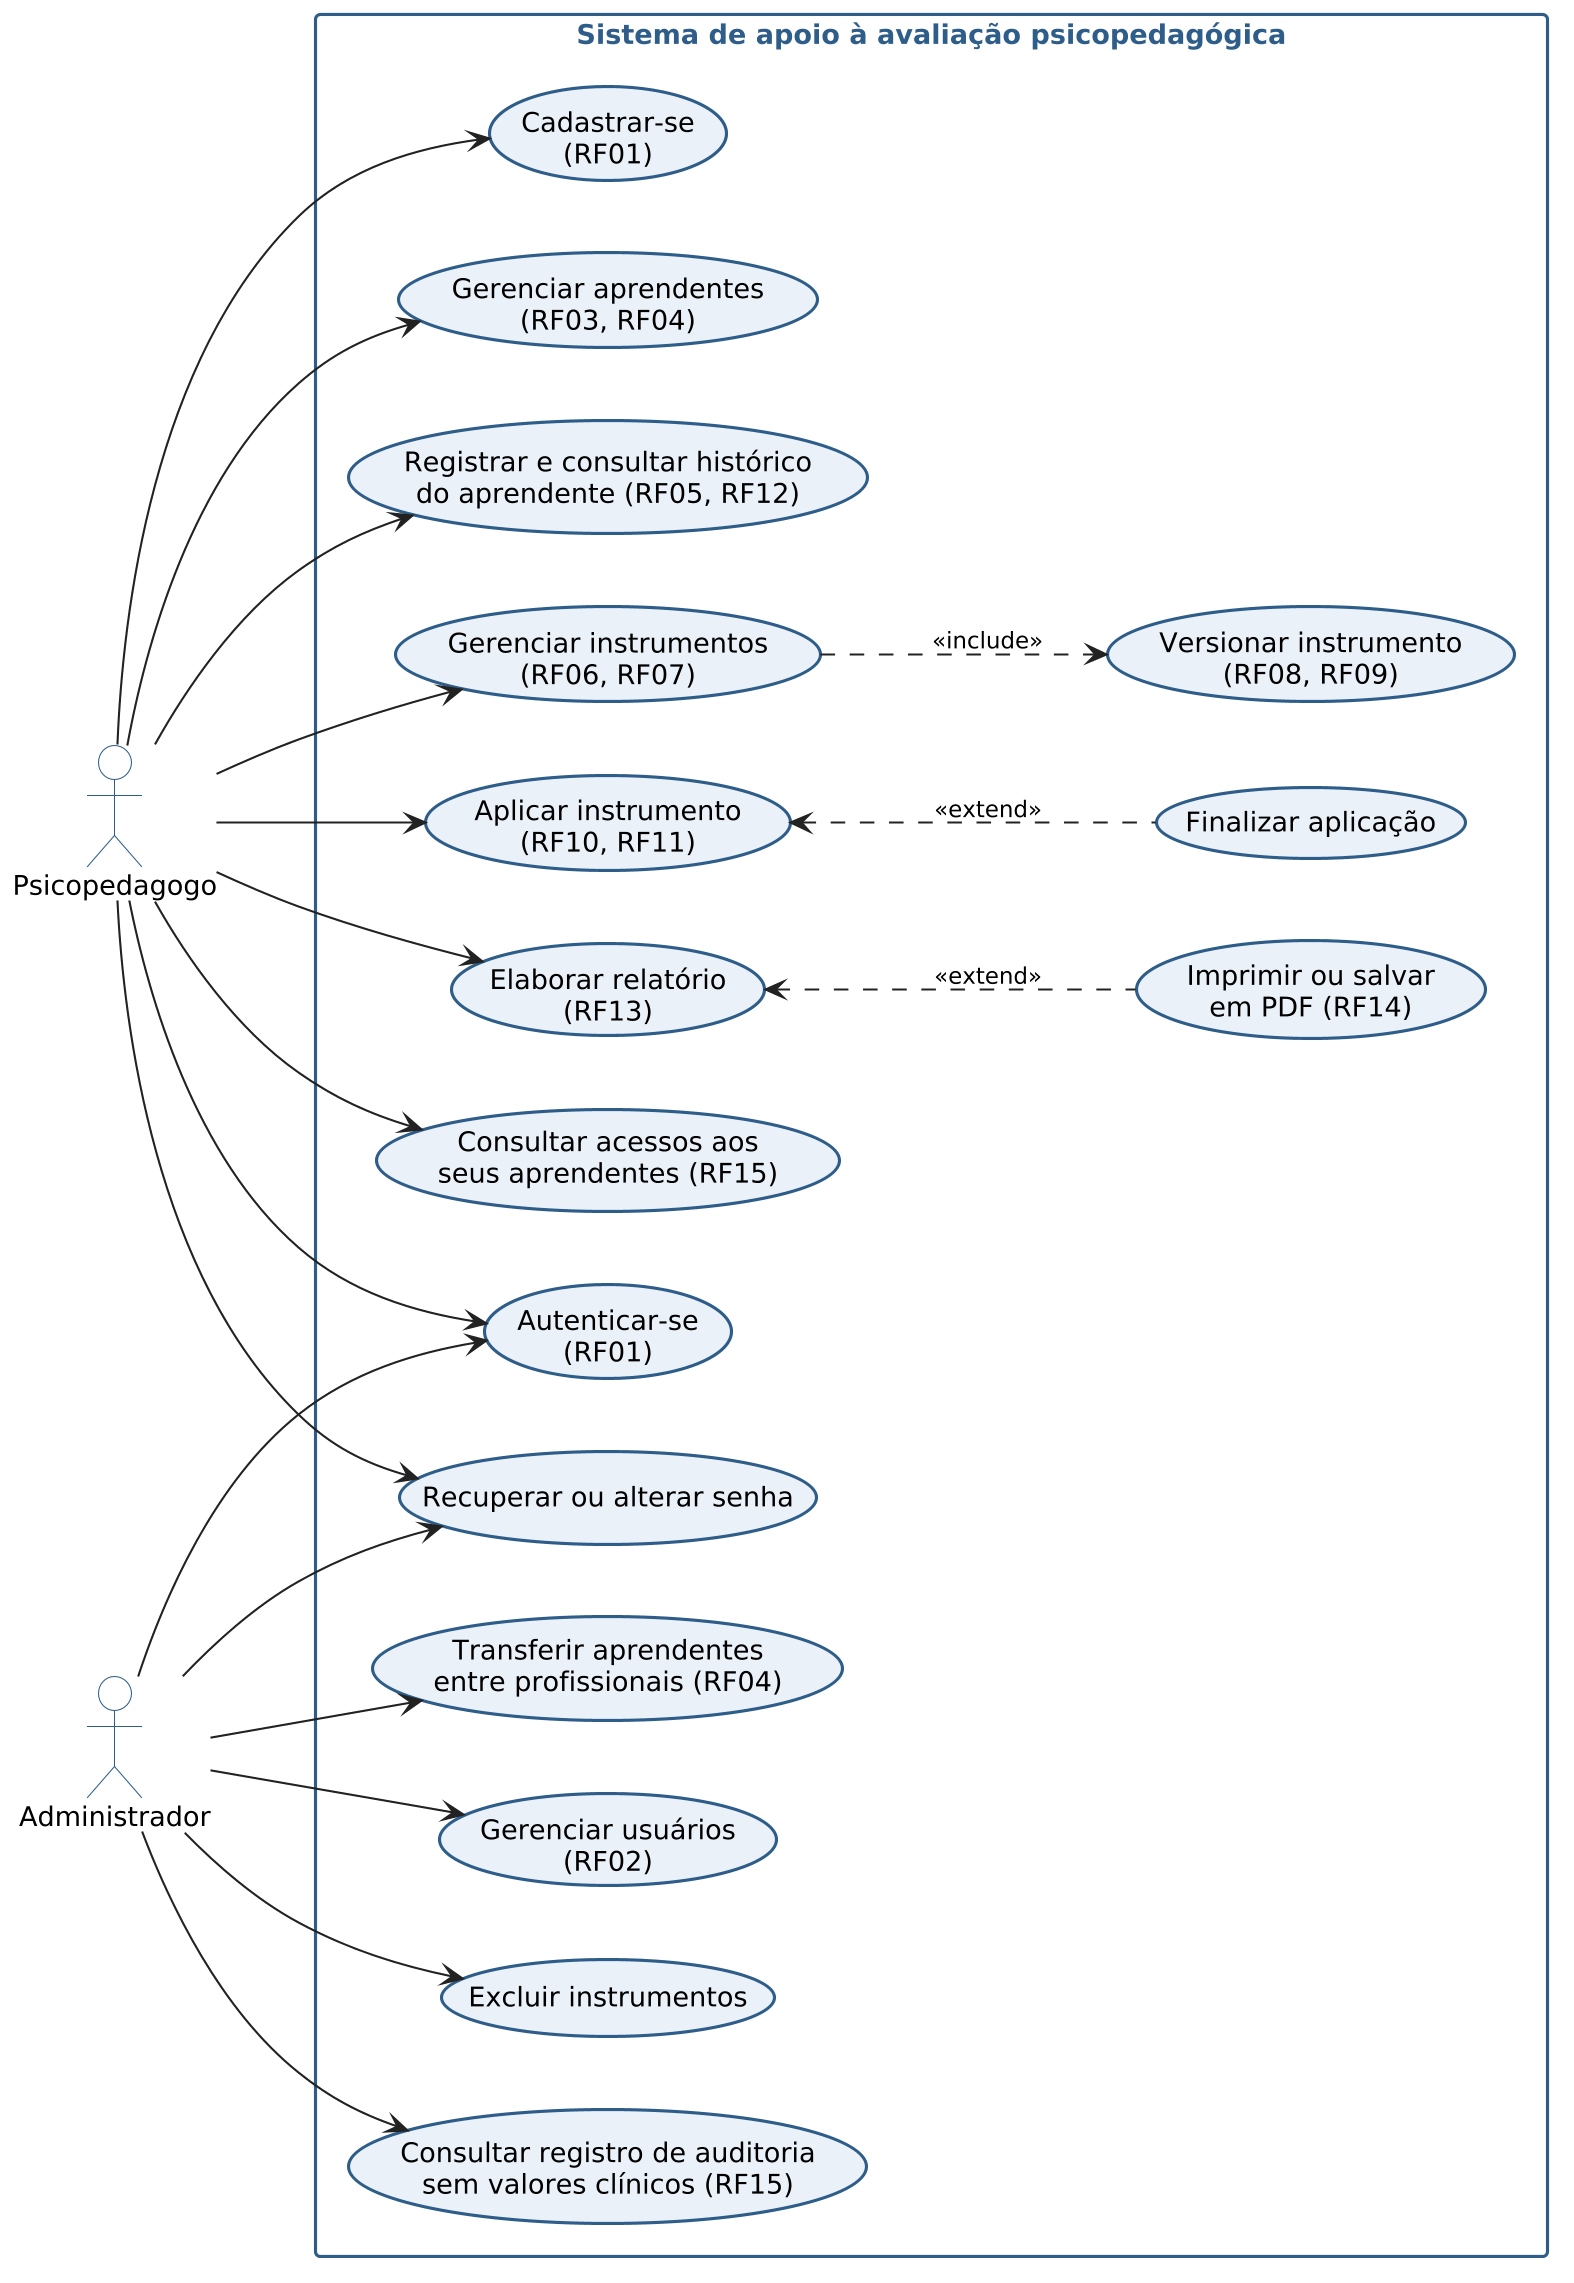
\includegraphics[width=\textwidth,height=0.75\textheight,keepaspectratio]{casos_de_uso.png}
    \fonte{Elaborado pela autora (2026).}
\end{figure}

\subsection{Requisitos não funcionais}

Os requisitos não funcionais (Quadro~\ref{qua:requisitos_nao_funcionais}) decorrem do fato de o sistema armazenar informações de crianças e priorizam segurança, privacidade, rastreabilidade e usabilidade. Seguindo a recomendação de expressá-los de forma mensurável (Seção~\ref{sec:fund_requisitos}), três receberam critérios de verificação: a usabilidade, avaliada por questionário com profissionais (RNF06); a acessibilidade, verificada pela ausência de violações das WCAG 2.2 \cite{w3c_wcag22_pt} detectáveis pela ferramenta axe-core \cite{deque_axe_core}, já que a conformidade plena depende de avaliação manual (RNF11); e a manutenibilidade, associada a uma cobertura mínima de testes no \textit{backend} (RNF10).

\begin{quadro}[H]
\centering
\footnotesize
\caption{Requisitos não funcionais}
\begin{tabular}{|p{1.6cm}|p{13cm}|}
\hline
\textbf{Código} & \textbf{Requisito não funcional} \\
\hline
RNF01 & O sistema deve utilizar autenticação para controlar o acesso dos usuários. \\ \hline
RNF02 & O sistema deve utilizar mecanismos de autorização para restringir o acesso às funcionalidades e informações, inclusive limitando a visualização de aprendentes e avaliações ao usuário responsável por cada registro. \\ \hline
RNF03 & Os dados dos aprendentes devem ser armazenados de forma segura, considerando os princípios de proteção de dados da LGPD. \\ \hline
RNF04 & O sistema deve manter um registro de auditoria que permita reconstituir quem criou, alterou, excluiu ou consultou cada dado, quando e com quais valores anteriores, inclusive nas operações realizadas pelo administrador. \\ \hline
RNF05 & O sistema deve preservar o histórico das versões e alterações realizadas nos instrumentos avaliativos. \\ \hline
RNF06 & A interface deve apresentar organização e usabilidade adequadas às atividades dos profissionais, verificada por meio de avaliação com usuários: média igual ou superior a 4,0 em escala de 1 a 5 nos aspectos de facilidade de uso, organização das informações e contribuição geral da plataforma. \\ \hline
RNF07 & A aplicação deve apresentar arquitetura em três camadas separadas (apresentação, aplicação e persistência), com o \textit{backend} organizado em módulos independentes por domínio funcional (autenticação, usuários, aprendentes, avaliações, aplicações, relatórios, auditoria e \textit{dashboard}), de modo que alterações em um módulo não exijam modificações nos demais. \\ \hline
RNF08 & Os dados devem possuir mecanismos de integridade e consistência durante seu armazenamento e manipulação. \\ \hline
RNF09 & O sistema deve possuir tratamento adequado de erros, evitando a exposição de informações internas da aplicação. \\ \hline
RNF10 & O sistema deve possuir cobertura de testes automatizados de no mínimo 70\% das linhas de código do \textit{backend}, de modo a permitir a detecção de regressões durante a evolução do sistema. \\ \hline
RNF11 & A interface não deve apresentar violações dos critérios de sucesso dos níveis A e AA das WCAG 2.2 detectáveis pela ferramenta axe-core nas telas principais do sistema. \\ \hline
\end{tabular}
\fonte{Elaborado pela autora (2026).}
\label{qua:requisitos_nao_funcionais}
\end{quadro}

\section{Arquitetura e modelo de dados}\label{sec:arquitetura_dados}

Esta seção apresenta a organização geral do sistema em camadas e, em seguida, o modelo de dados que sustenta o processo avaliativo.

\subsection{Arquitetura do sistema}\label{sec:arquitetura}

O sistema adota a arquitetura em três camadas discutida na Seção~\ref{sec:fund_arquitetura}: apresentação, aplicação e persistência. Essa organização separa a interface usada pelo profissional, as regras de negócio e o armazenamento dos dados.

A camada de apresentação é o \textit{frontend}, desenvolvido em React como uma aplicação de página única. Ela reúne as telas destinadas ao psicopedagogo (aprendentes, instrumentos, aplicações e relatórios) e as destinadas ao administrador (usuários e registro de auditoria). A comunicação com o servidor ocorre por meio de uma API REST desenvolvida em Node.js com Express. Seguindo o estilo REST \cite{fielding2000_rest}, a API não mantém estado de sessão: cada requisição carrega o \textit{token} de acesso do usuário, e as operações são expressas pelos métodos e códigos de estado do HTTP.

Na camada de aplicação, cada requisição passa pela autenticação, que identifica o usuário a partir do \textit{token}, pela autorização por perfil e pela validação dos dados antes de chegar aos módulos de negócio: autenticação (\textit{auth}), usuários (\textit{users}), aprendentes (\textit{aprendentes}), instrumentos avaliativos (\textit{avaliacoes}), aplicações dos instrumentos (\textit{aplicacoes}), relatórios (\textit{relatorios}), painel geral (\textit{dashboard}) e auditoria (\textit{auditoria}). Como todas as decisões de acesso são tomadas nessa camada, o controle não depende do que a interface exibe ao usuário. O registro de auditoria fica na fronteira entre a aplicação e a persistência: as operações sobre o banco passam por uma extensão do Prisma que registra quem as realizou, quando e sobre qual dado (Seção~\ref{sec:auditoria}).

A camada de persistência utiliza o banco de dados relacional MySQL, que armazena os usuários, os aprendentes e seu histórico, os instrumentos e suas questões, as aplicações e respostas, os relatórios e o registro de auditoria.

Para execução, os serviços (banco de dados, API e \textit{frontend}) são executados em contêineres Docker. O Nginx entrega os arquivos estáticos do \textit{frontend} ao navegador e atua como \textit{proxy} reverso, encaminhando à API as requisições dirigidas a ela. Essa configuração foi utilizada no ambiente local de testes e de avaliação; o sistema não foi implantado em ambiente de produção (Seção~\ref{sec:limitacoes}).

A Figura~\ref{fig:arquitetura_geral_do_sistema} resume a arquitetura e indica também a separação entre os perfis: os módulos em destaque reúnem dados clínicos e são exclusivos do psicopedagogo responsável, enquanto o administrador atua na gestão de usuários e na auditoria, sem acesso a esses dados (Seção~\ref{sec:separacao_admin}).

\begin{figure}[H]
    \centering
    \caption{Arquitetura geral do sistema}
    \label{fig:arquitetura_geral_do_sistema}
    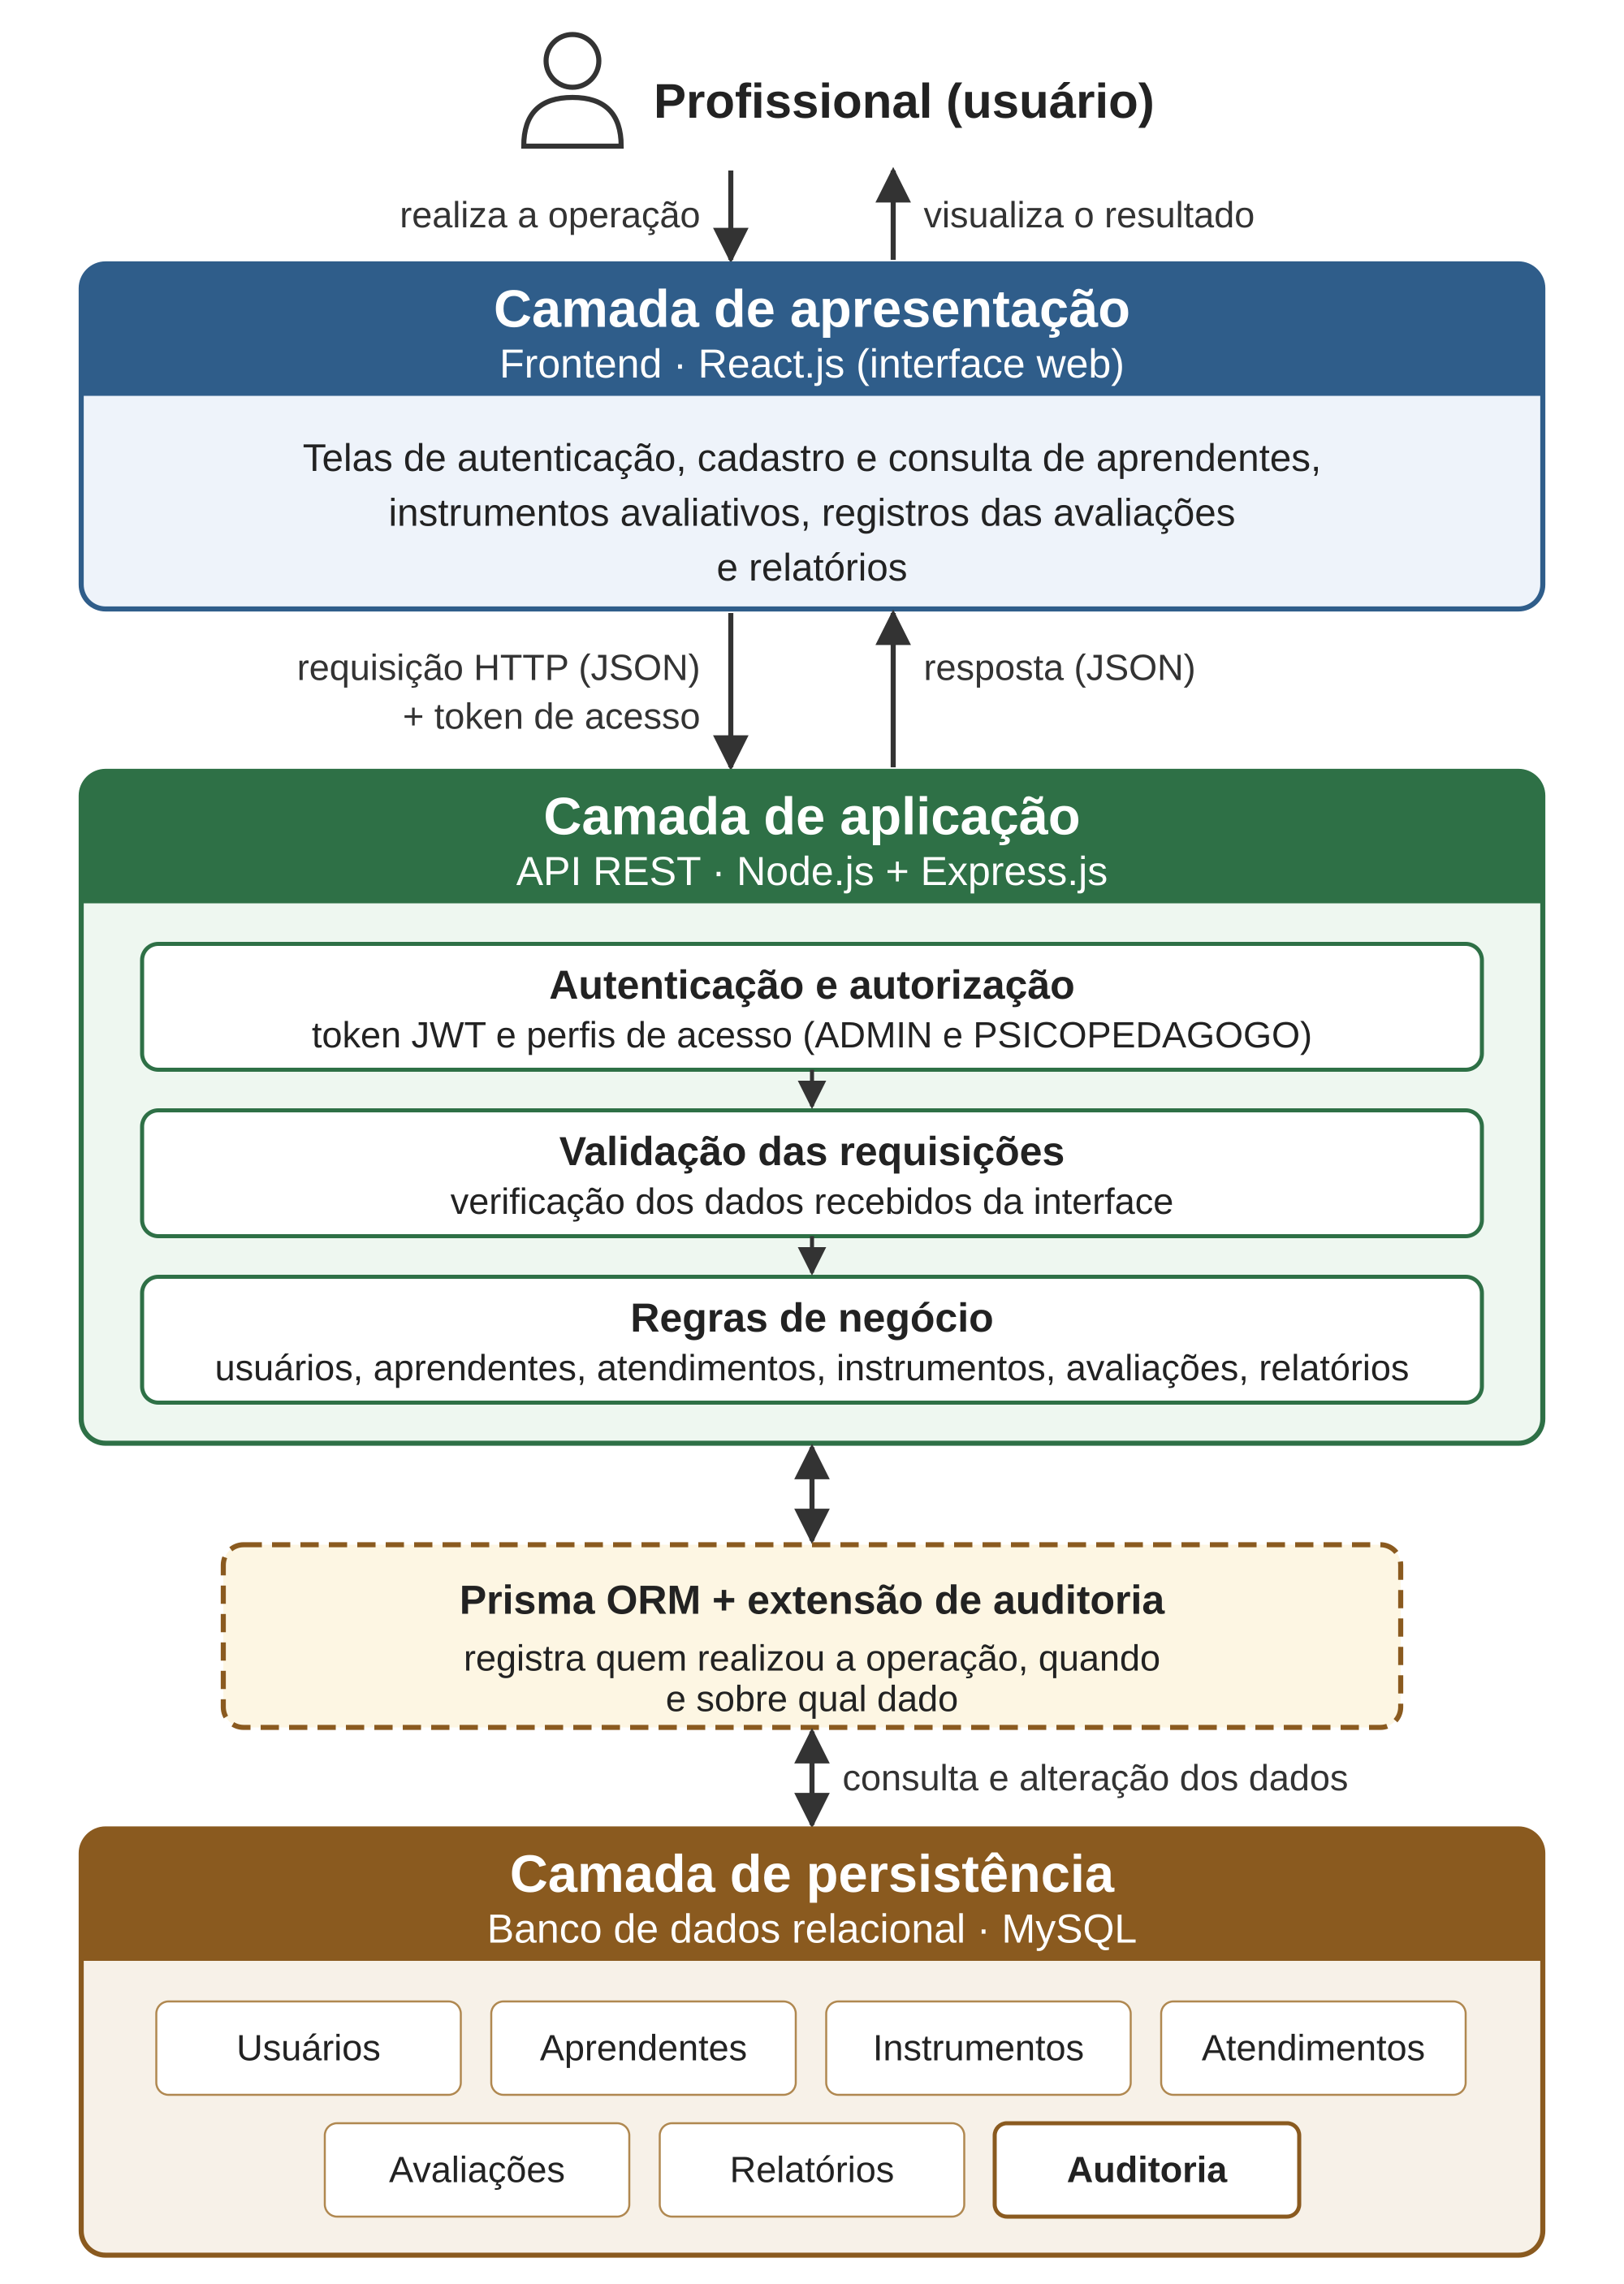
\includegraphics[width=\textwidth,height=0.7\textheight,keepaspectratio]{arquitetura_sistema.png}
    \fonte{Elaborado pela autora (2026).}
\end{figure}


\subsection{Modelo de dados}\label{sec:modelagem}

O banco de dados foi implementado em MySQL segundo o modelo relacional \cite{codd1970_relational}, representado por meio do modelo entidade-relacionamento \cite{chen1976_entity_relationship} e acessado pela aplicação por meio do Prisma (Seção~\ref{sec:fund_banco}). O modelo tem onze entidades, apresentadas em duas partes nas Figuras~\ref{fig:der_parte1} e \ref{fig:der_parte2}. Quanto à nomenclatura, cabe observar que a entidade \textit{avaliacoes} representa os \textbf{instrumentos} avaliativos, e a entidade \textit{aplicacoes}, cada uso de um instrumento com um aprendente; no texto, os termos ``instrumento'' e ``aplicação'' são usados nesses sentidos.

A primeira parte reúne os usuários e a autenticação (\textit{users}, \textit{refresh\_tokens} e \textit{password\_resets}), os aprendentes e seu histórico (\textit{aprendentes} e \textit{historico\_aprendentes}) e o registro de auditoria (\textit{audit\_logs}). A segunda reúne o processo avaliativo: instrumentos (\textit{avaliacoes}), questões (\textit{questions}), aplicações (\textit{aplicacoes}), respostas (\textit{respostas}) e relatórios (\textit{relatorios}). As principais decisões de modelagem são descritas a seguir.

\begin{itemize}
    \item \textbf{Titularidade}: os campos \textit{responsavelId}, em \textit{aprendentes}, e \textit{autorId}, em \textit{avaliacoes}, vinculam cada registro ao profissional responsável e sustentam a restrição de visibilidade (Seção~\ref{sec:titularidade}). Ambos são indexados, pois as listagens filtram os registros pelo usuário autenticado.
    \item \textbf{Versionamento}: o campo \textit{parentId} cria uma autorrelação em \textit{avaliacoes}, de modo que cada nova versão de um instrumento aponta para a anterior (Seção~\ref{sec:instrumentos}).
    \item \textbf{Questões configuráveis}: cada questão tem texto, tipo, obrigatoriedade e posição, com oito tipos de resposta (texto curto e longo, número, data, seleção única e múltipla, escala e sim/não). Assim, novos instrumentos não exigem alterações na estrutura do banco.
    \item \textbf{Respostas em JSON}: o campo \textit{valor} de \textit{respostas} é do tipo JSON, o que permite guardar formatos diferentes conforme o tipo da questão. Uma restrição de unicidade sobre o par \textit{aplicacaoId} e \textit{questionId} impede duas respostas para a mesma questão em uma aplicação.
    \item \textbf{Relatório vinculado à aplicação}: cada relatório pertence a uma única aplicação, em uma relação de zero ou um, o que o mantém associado ao instrumento e à versão utilizados.
    \item \textbf{Auditoria independente}: \textit{audit\_logs} registra o usuário e seu perfil, a ação, a entidade e o registro afetados, o aprendente a que o dado pertence, o IP, o momento e, quando houver, as diferenças entre os valores anteriores e os novos. A entidade não tem chave estrangeira para \textit{users}, para que o registro não dependa de alterações posteriores no cadastro de usuários.
    \item \textbf{Exclusão lógica}: usuários, aprendentes e instrumentos têm o campo \textit{deletedAt}, de modo que as exclusões não apagam fisicamente os registros.
\end{itemize}

\begin{figure}[H]
    \centering
    \caption{Diagrama Entidade-Relacionamento do sistema (parte 1): usuários, aprendentes e auditoria}
    \label{fig:der_parte1}
    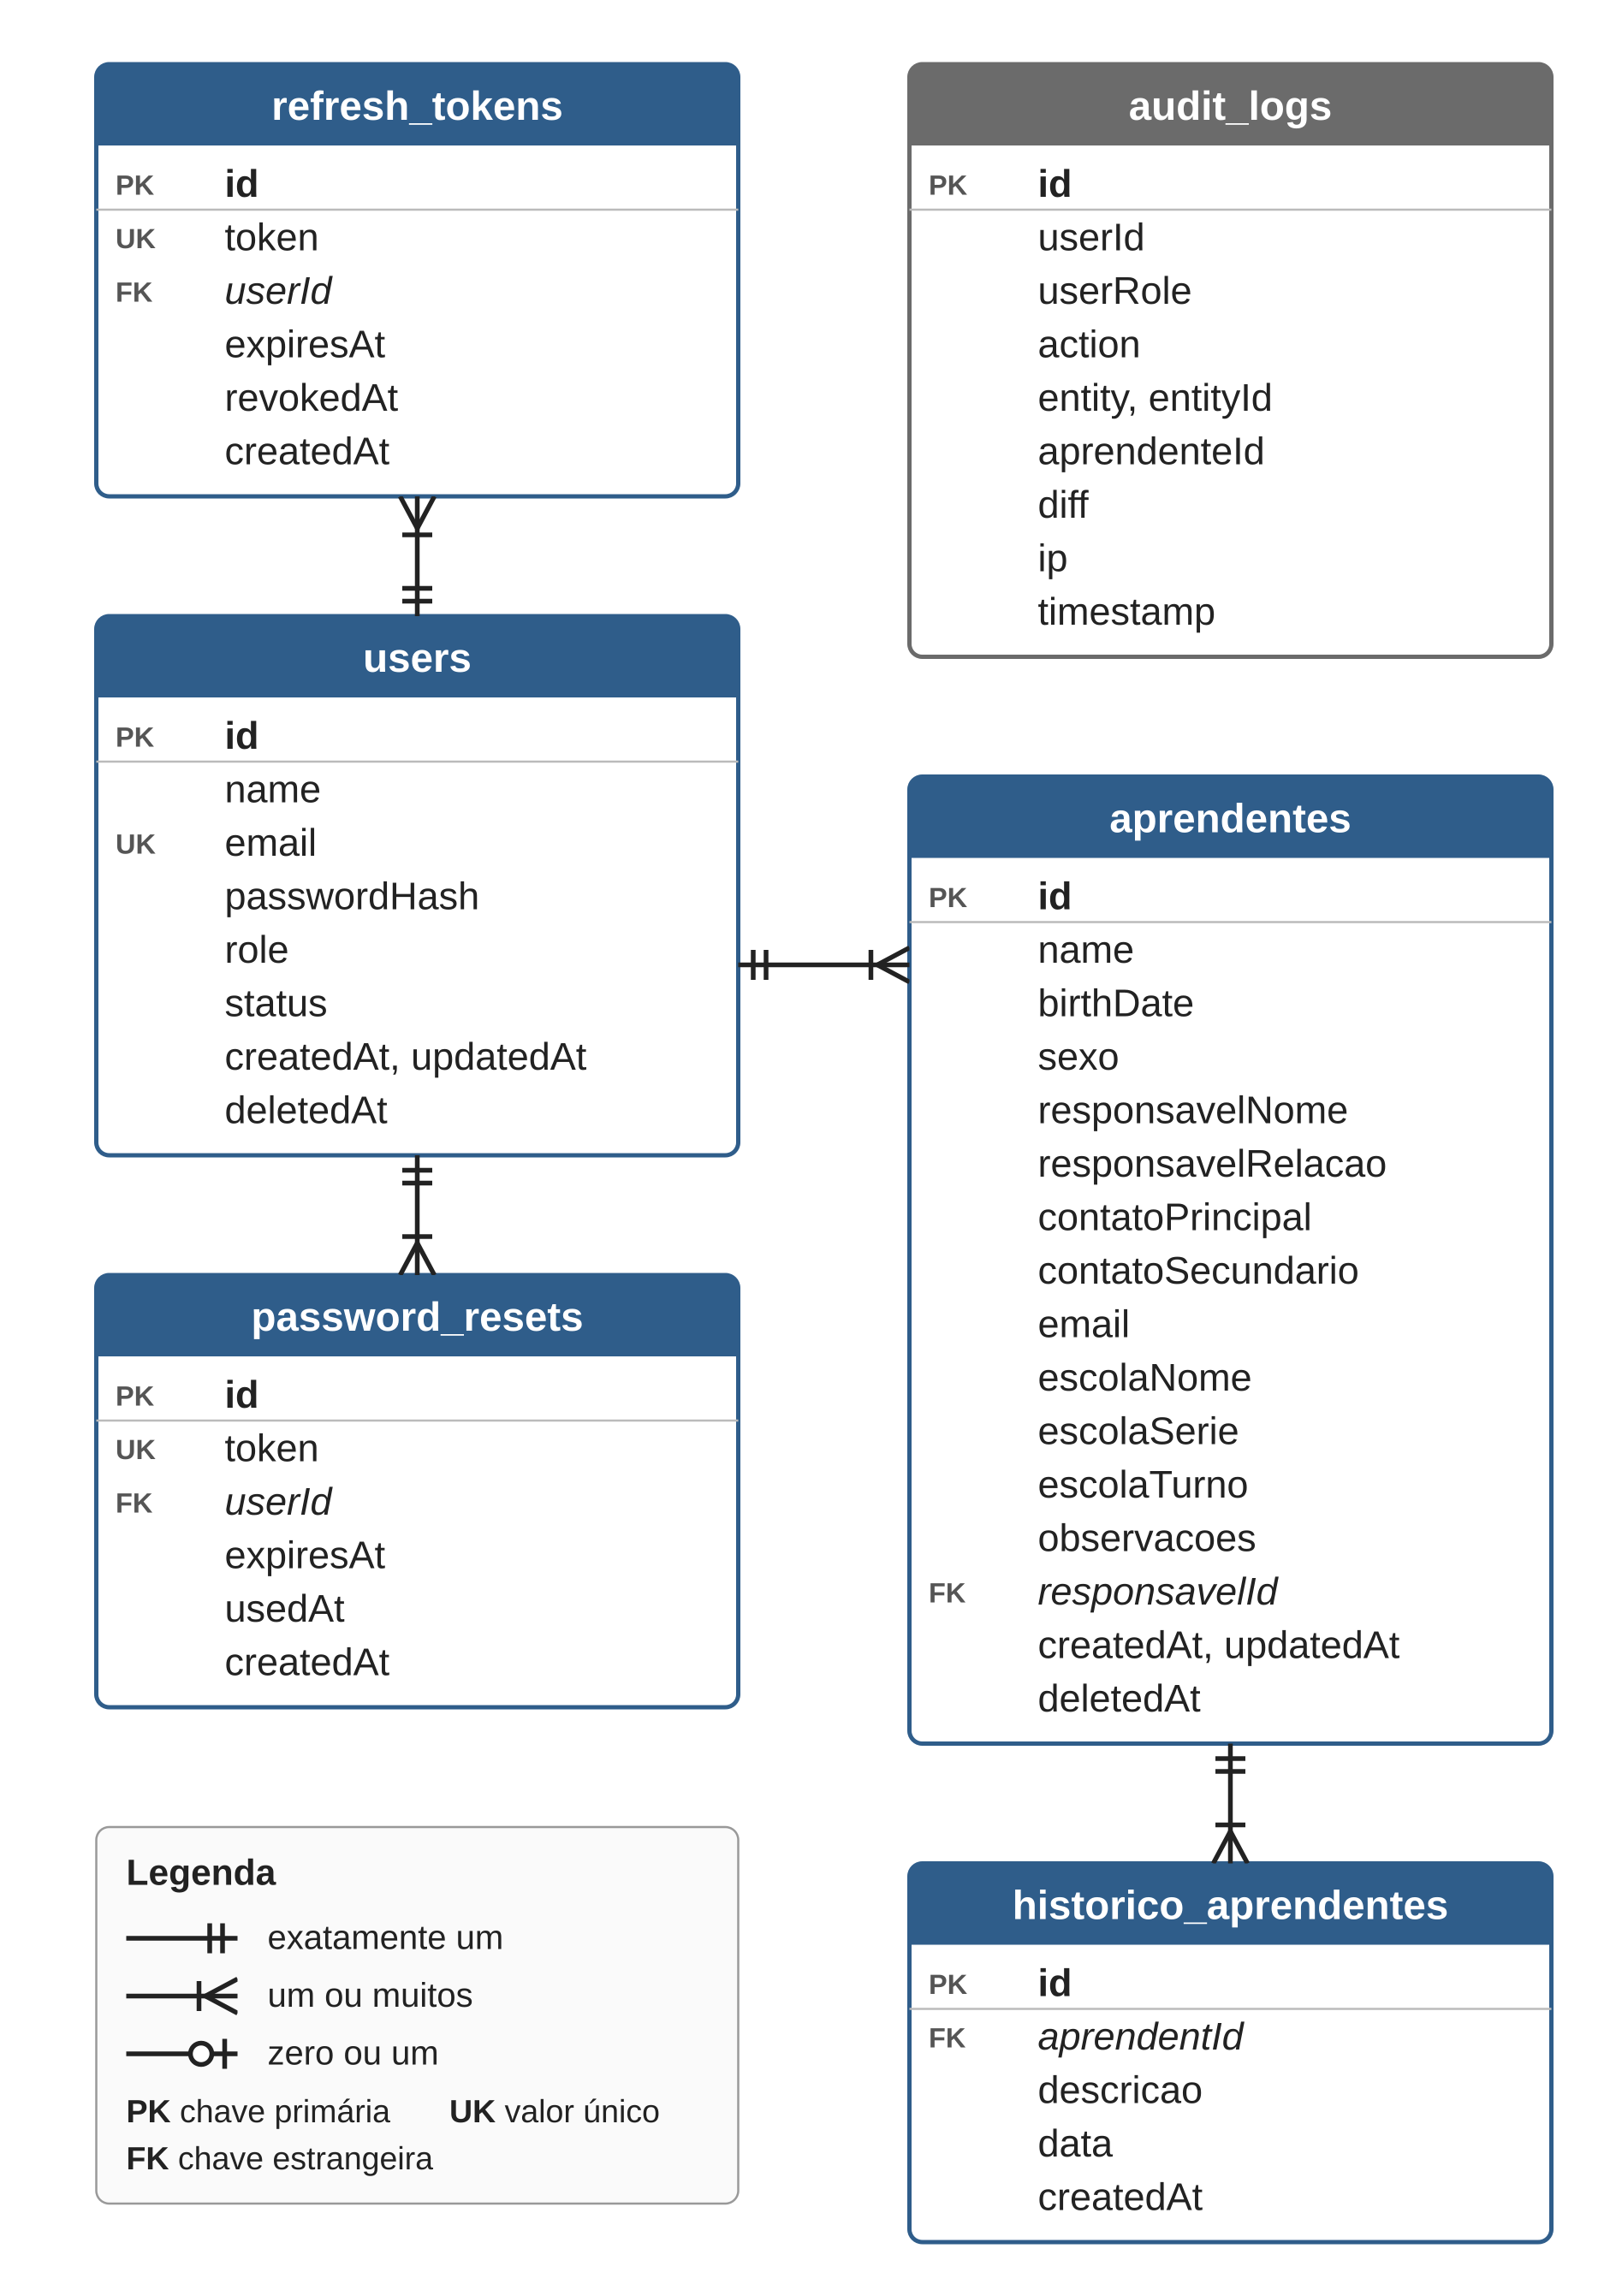
\includegraphics[width=\textwidth,height=0.6\textheight,keepaspectratio]{der_parte1.png}
    \fonte{Elaborado pela autora (2026).}
\end{figure}

Na Figura~\ref{fig:der_parte2}, as entidades \textit{users} e \textit{aprendentes}, detalhadas na primeira parte, aparecem em linha tracejada, apenas para indicar seus relacionamentos.

\begin{figure}[H]
    \centering
    \caption{Diagrama Entidade-Relacionamento do sistema (parte 2): instrumentos, aplicações e relatórios}
    \label{fig:der_parte2}
    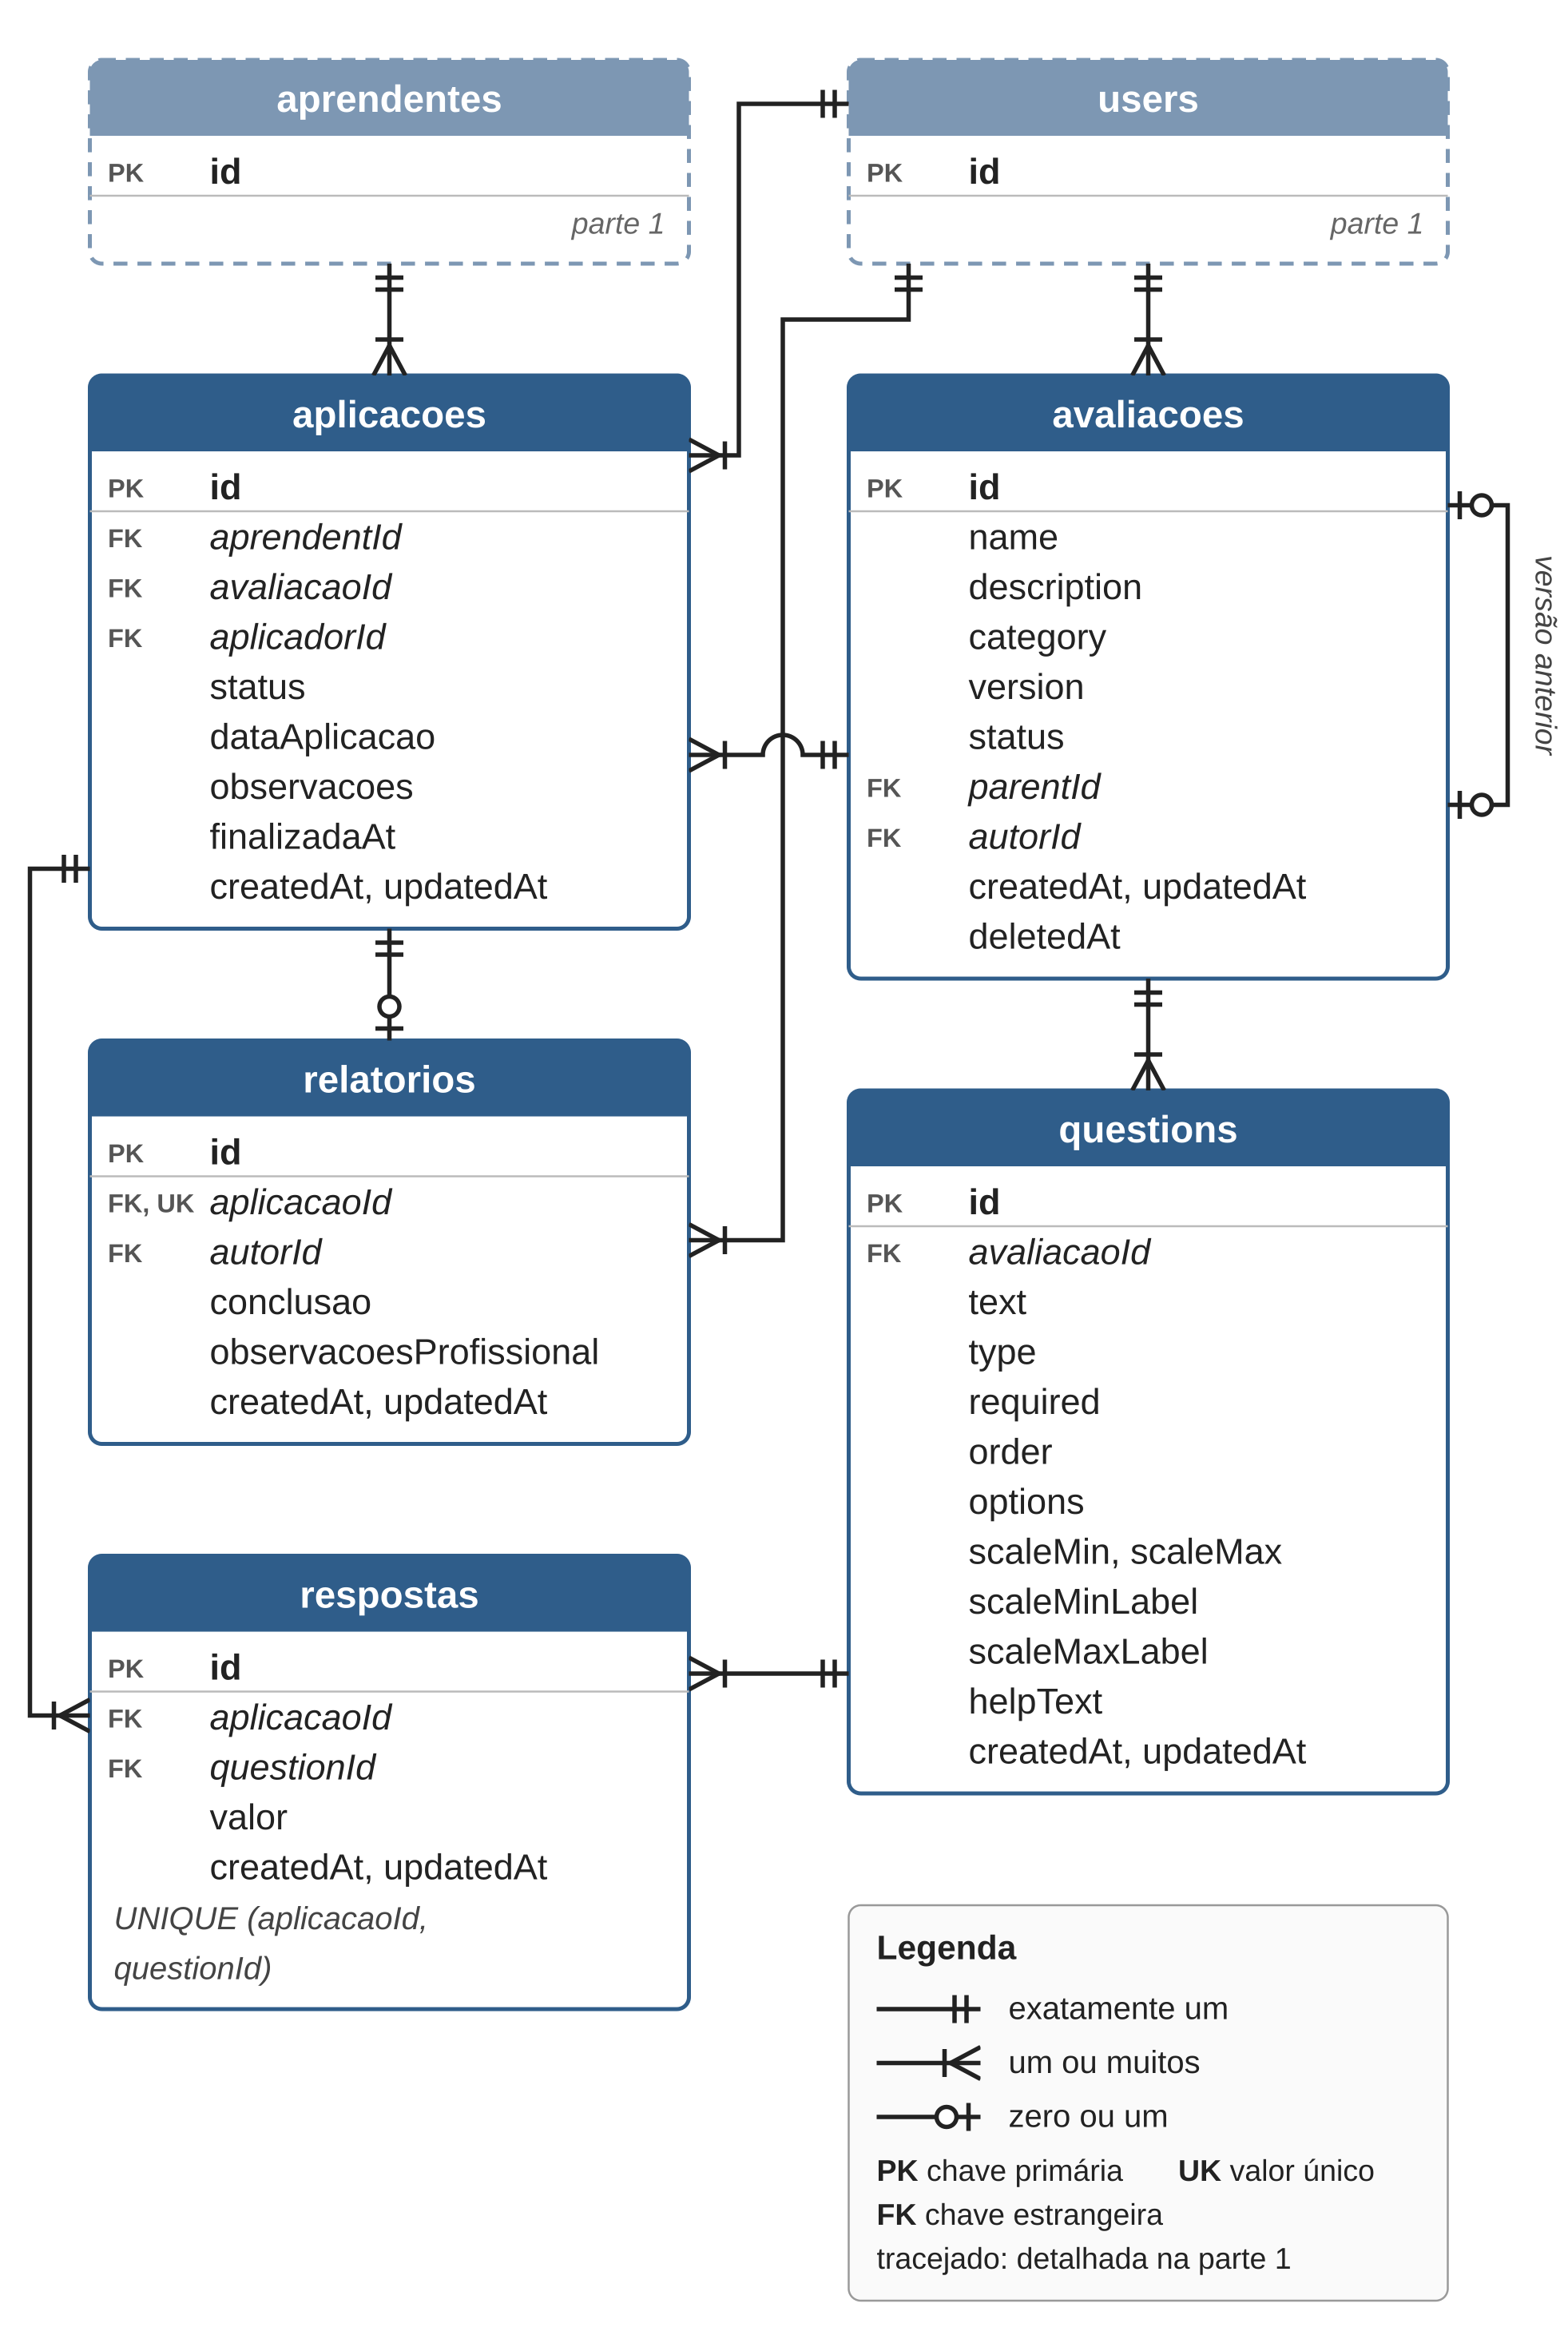
\includegraphics[width=\textwidth,height=0.6\textheight,keepaspectratio]{der_parte2.png}
    \fonte{Elaborado pela autora (2026).}
\end{figure}


\section{Desenvolvimento do \textit{backend}}\label{sec:backend}

O \textit{backend} foi desenvolvido em Node.js com Express, com persistência em MySQL por meio do Prisma, validação de dados com Zod e documentação da API no padrão Swagger/OpenAPI, disponível no endereço \textit{/api-docs}. A aplicação está organizada em módulos de negócio, um por domínio funcional (Seção~\ref{sec:arquitetura}), cada um com suas rotas, controladores e serviços. Antes dos controladores, as requisições passam por \textit{middlewares} de autenticação, de validação dos dados contra os esquemas Zod e de tratamento centralizado de erros, que evita expor detalhes internos da aplicação nas respostas.

\subsection{Rotas da API}

As rotas da API são agrupadas por domínio funcional, e o controle de acesso por perfil é aplicado antes do processamento de cada requisição. O Quadro~\ref{qua:rotas_api} apresenta uma seleção das rotas que ilustram esse controle; a lista completa está na documentação Swagger do sistema.

\begin{quadro}[H]
\centering
\footnotesize
\caption{Seleção de rotas da API REST e perfil exigido}
\begin{tabular}{|p{1.4cm}|p{5.6cm}|p{2.4cm}|p{4.8cm}|}
\hline
\textbf{Método} & \textbf{Rota} & \textbf{Perfil exigido} & \textbf{Descrição} \\ \hline
POST & /api/auth/login & Público & Autenticação e emissão dos \textit{tokens} \\ \hline
POST & /api/auth/refresh & Público & Renovação do \textit{token} de acesso \\ \hline
GET & /api/users & ADMIN & Listagem de usuários \\ \hline
POST & /api/users/:id/transferir-aprendentes & ADMIN & Transferência dos aprendentes e instrumentos para outro psicopedagogo \\ \hline
GET & /api/aprendentes/:id & Psicopedagogo & Consulta de aprendente \\ \hline
POST & /api/avaliacoes & Autenticado\textsuperscript{*} & Cadastro de instrumento \\ \hline
PUT & /api/avaliacoes/:id & Psicopedagogo & Edição de instrumento (cria nova versão se já aplicado) \\ \hline
DELETE & /api/avaliacoes/:id & ADMIN & Exclusão de instrumento \\ \hline
POST & /api/aplicacoes/:id/finalize & Psicopedagogo & Finalização da aplicação \\ \hline
POST & /api/relatorios & Psicopedagogo & Criação ou atualização de relatório \\ \hline
GET & /api/dashboard & Autenticado & Painel geral (para o ADMIN, apenas totais) \\ \hline
GET & /api/auditoria & Autenticado & Registro de auditoria (para o ADMIN, sem valores clínicos) \\ \hline
\end{tabular}
\fonte{Elaborado pela autora (2026). \textsuperscript{*}A rota exige apenas autenticação, mas o cadastro é recusado ao ADMIN dentro do módulo de instrumentos, e não pelo \textit{middleware} de perfil.}
\label{qua:rotas_api}
\end{quadro}

\subsection{Autenticação e controle de acesso}

A autenticação foi implementada utilizando JWT \cite{rfc7519_jwt}, com tokens de acesso (\textit{access token}) e de renovação (\textit{refresh token}), conforme o esquema descrito na Seção~\ref{sec:fund_seguranca}. Os \textit{tokens} são assinados com o algoritmo HMAC SHA-256, padrão da biblioteca \textit{jsonwebtoken}, utilizando chaves secretas distintas para cada tipo de token. O \textit{access token} tem validade de 15 minutos, e o \textit{refresh token}, de 7 dias. Ambos os valores são configuráveis por variável de ambiente.

No \textit{frontend}, os \textit{tokens} são armazenados no \textit{localStorage} do navegador. Essa escolha simplifica a implementação, mas expõe os tokens a ataques de \textit{cross-site scripting} (XSS); a alternativa mais segura seria o uso de \textit{cookies httpOnly}, que não são acessíveis por JavaScript. Essa é uma limitação do protótipo para uso em produção.

O \textit{refresh token} é rotacionado a cada uso: o anterior é revogado no banco de dados e um novo é emitido. Ele é armazenado em texto plano na tabela \textit{refresh\_tokens}, e não como \textit{hash}, o que é outra limitação reconhecida. No \textit{logout}, o \textit{token} é revogado imediatamente, e na redefinição de senha todos os \textit{refresh tokens} ativos do usuário são revogados em uma única transação, encerrando sessões abertas em outros dispositivos.

A Figura~\ref{fig:sequencia_login} apresenta, em um diagrama de sequência da UML \cite{omg2017_uml}, as três situações do ciclo de autenticação. No \textit{login} (passos 1 a 10), a API confere a senha com o bcrypt, emite os dois \textit{tokens}, grava o \textit{refresh token} e registra o acesso na auditoria. Nas requisições seguintes (passos 11 a 16), o \textit{middleware} \textit{authenticate} valida o \textit{access token} enviado no cabeçalho \textit{Authorization}, confere se o usuário continua ativo e disponibiliza seu identificador e perfil aos serviços, que aplicam o filtro de titularidade.

\begin{figure}[H]
    \centering
    \caption{Diagrama de sequência da autenticação com \textit{access token} e \textit{refresh token}}
    \label{fig:sequencia_login}
    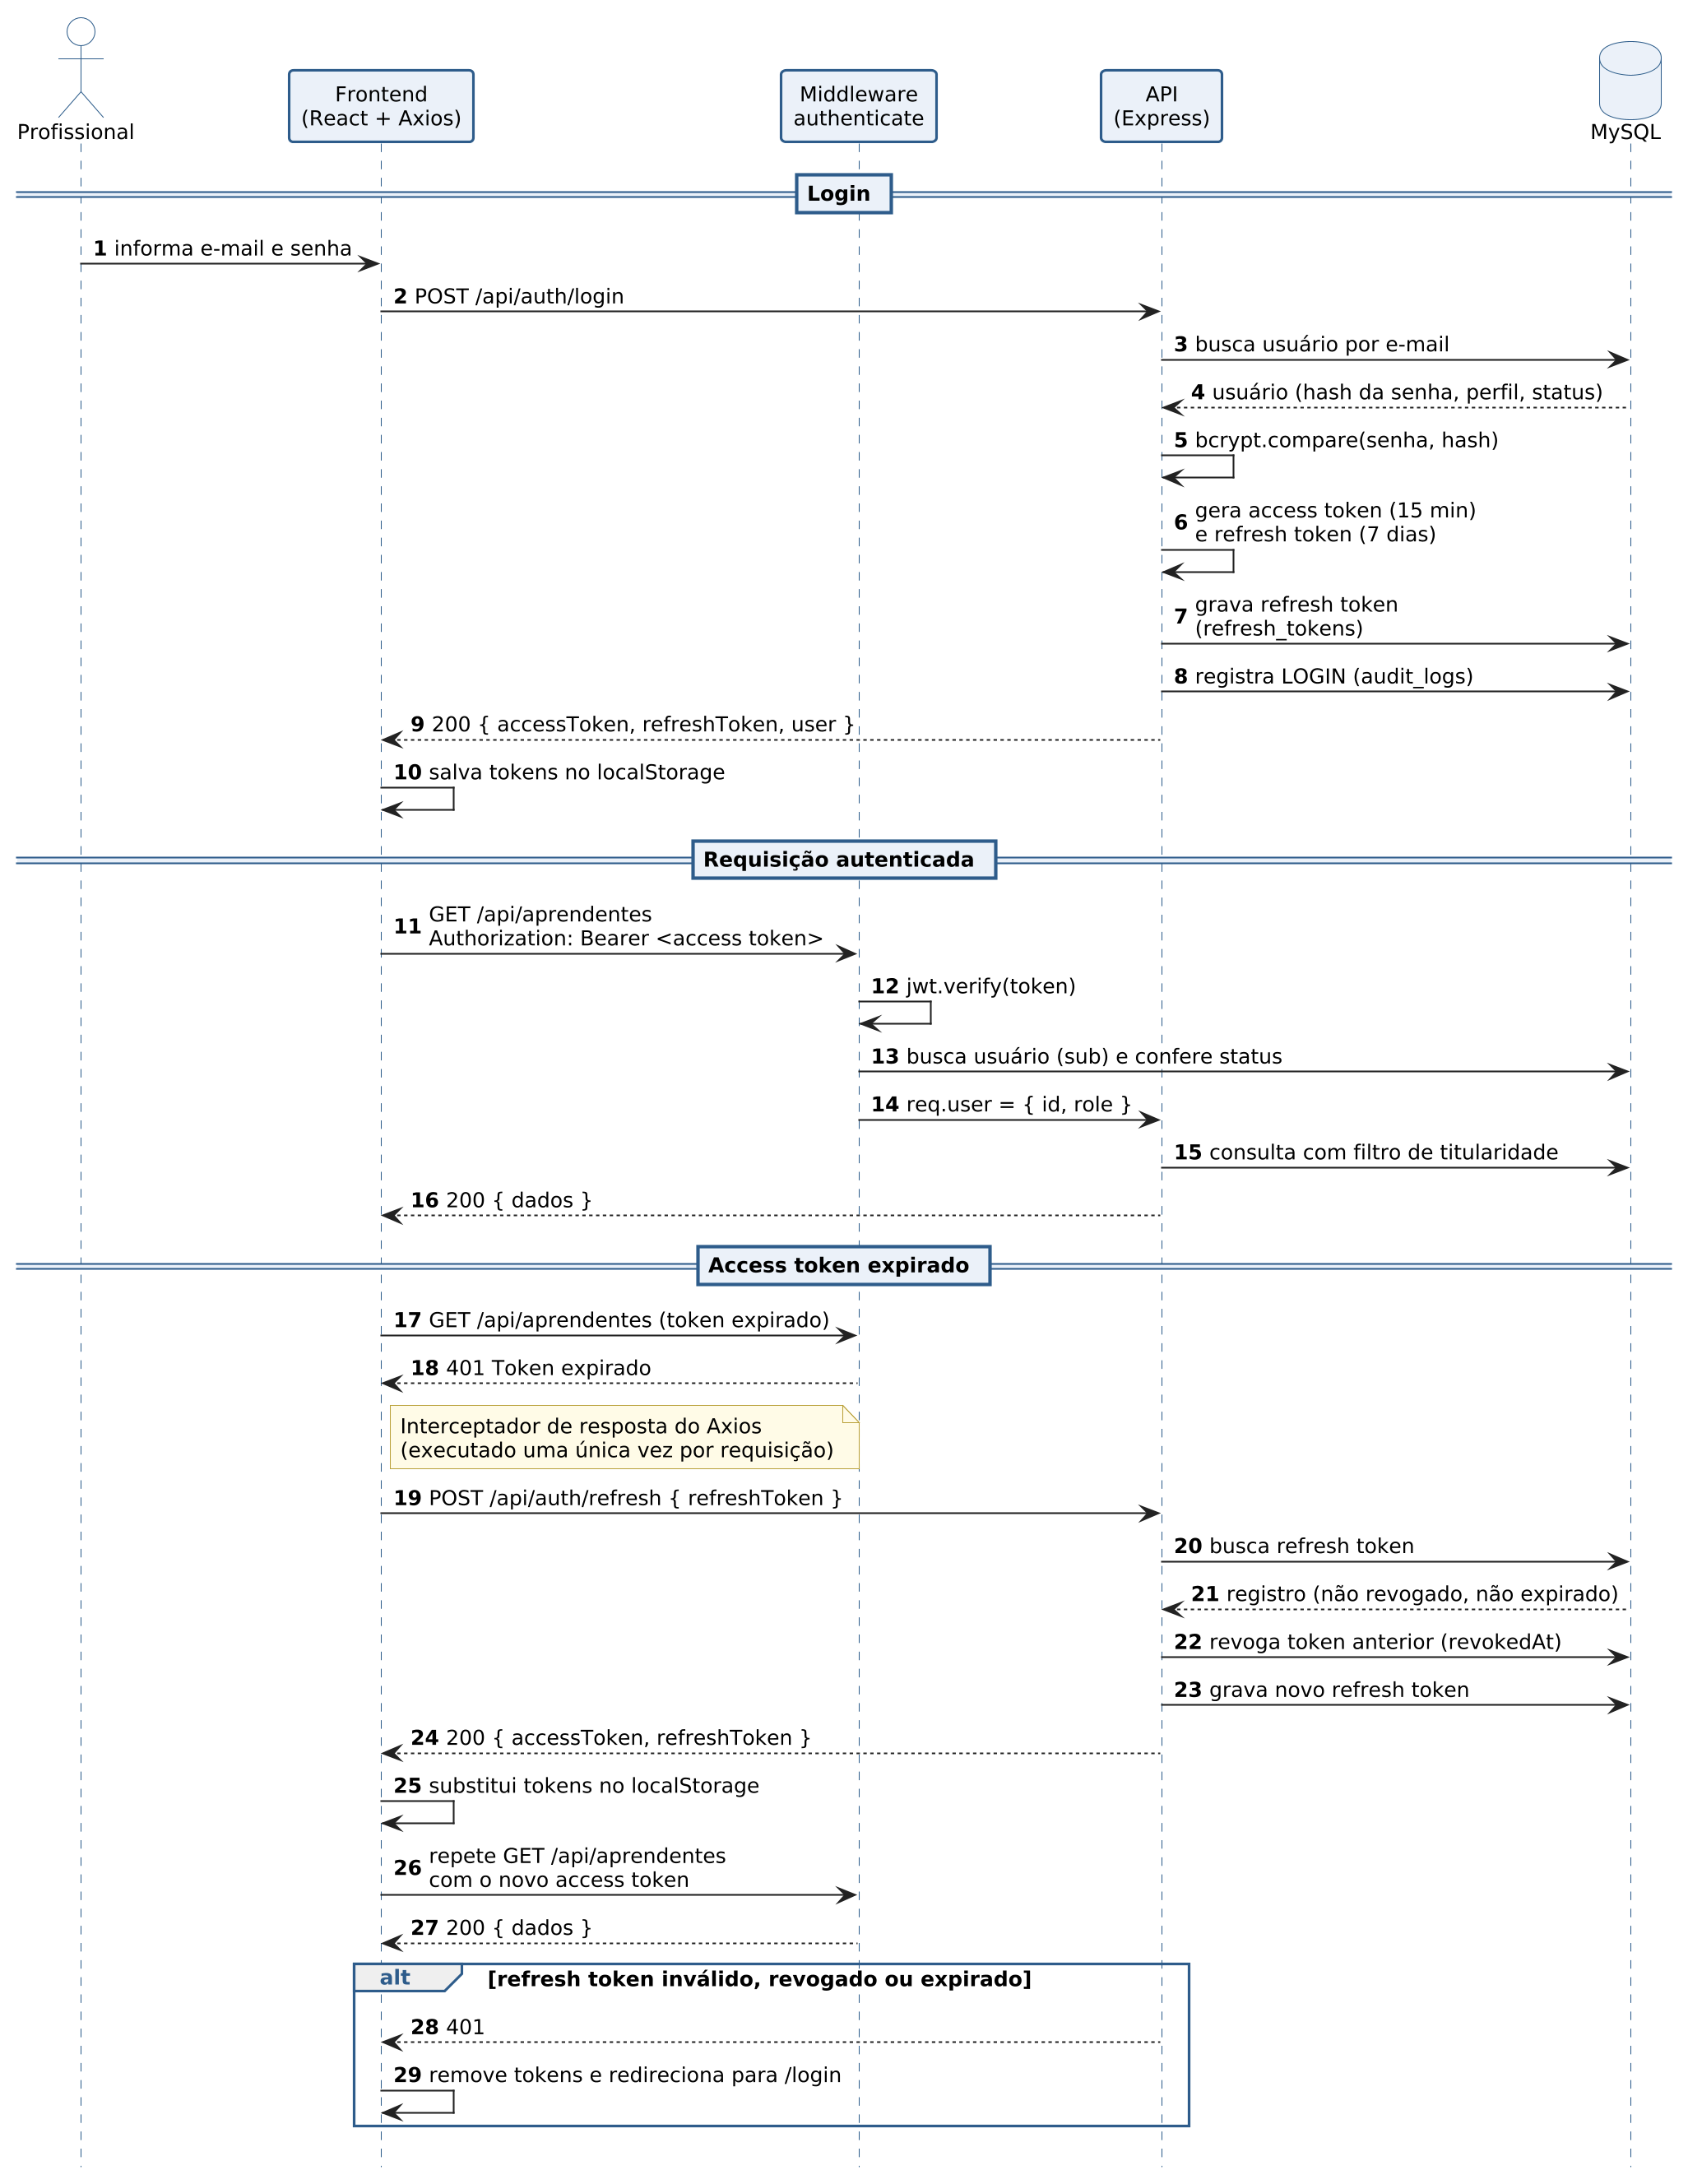
\includegraphics[width=0.92\textwidth,height=0.78\textheight,keepaspectratio]{sequencia_login.png}
    \fonte{Elaborado pela autora (2026).}
\end{figure}

Quando o \textit{access token} expira (passos 17 a 27), a API responde com HTTP 401, e um interceptador do Axios no \textit{frontend} solicita automaticamente um novo par de \textit{tokens} à rota \textit{/api/auth/refresh}, repetindo a requisição original sem que o usuário perceba. Esse interceptador é executado uma única vez por requisição; se a renovação falhar, porque o \textit{refresh token} foi revogado ou expirou, os \textit{tokens} são removidos e o usuário é redirecionado para a tela de login (passos 28 e 29).

A recuperação de senha utiliza um \textit{token} gerado com \texttt{crypto.randomBytes(32)}, com validade de 1 hora. O link de redefinição é enviado por e-mail por meio do Nodemailer, configurado com servidor SMTP definido em variáveis de ambiente. Depois de usado, o \textit{token} é marcado como utilizado, o que impede sua reutilização.

Contra ataques de força bruta e abuso da API, o \textit{backend} aplica limitação de taxa (\textit{rate limiting}) globalmente por meio da biblioteca \textit{express-rate-limit}: no máximo 100 requisições por endereço IP em uma janela de 15 minutos. Ao atingir o limite, a API retorna HTTP 429 com mensagem de erro. Os valores são configuráveis por variável de ambiente.

O \textit{backend} contempla os perfis \textit{ADMIN} e \textit{PSICOPEDAGOGO}, com controle de acesso por perfil aplicado pelo \textit{middleware} \textit{authorize} nas rotas que exigem permissão específica, na forma de um controle de acesso baseado em papéis \cite{sandhu1996_rbac}. Como esse modelo não expressa restrições que dependem do registro acessado, o sistema o complementa com uma restrição baseada em um atributo do recurso, a titularidade, à maneira do controle de acesso baseado em atributos \cite{hu2014_abac}: aprendentes e instrumentos são vinculados ao usuário que os criou, e aplicações e relatórios seguem a titularidade do aprendente a que pertencem. As operações de leitura e escrita alcançam somente os registros pertencentes ao usuário autenticado. A combinação dos dois mecanismos é discutida na Seção~\ref{sec:seguranca}.

O Código~\ref{cod:authorize} apresenta o \textit{middleware} \textit{authorize} e seu uso em dois módulos: nas rotas de usuários, restritas ao \textit{ADMIN}, e nas de aprendentes, restritas ao \textit{PSICOPEDAGOGO} em todas as operações, inclusive nas de leitura. A função recebe a lista de perfis autorizados e devolve um \textit{middleware} do Express, que é executado depois do \textit{authenticate} e, portanto, já encontra em \textit{req.user} o usuário validado a partir do \textit{token}. A distinção entre as duas respostas de erro segue a semântica do HTTP: 401 indica que a requisição não está autenticada, e 403, que o usuário está autenticado mas não possui o perfil exigido.

\begin{lstlisting}[caption={Middleware \textit{authorize} e sua aplicação nas rotas de usuários e de aprendentes},label={cod:authorize}]
// apps/backend/src/middlewares/auth.middleware.js
const authorize = (...roles) => {
  return (req, res, next) => {
    if (!req.user) {
      return res.status(401).json({ success: false, message: 'Não autenticado' });
    }
    if (!roles.includes(req.user.role)) {
      return res.status(403).json({ success: false, message: 'Acesso negado' });
    }
    next();
  };
};

// apps/backend/src/modules/users/users.routes.js
router.use(authenticate);
router.get('/', authorize('ADMIN'), controller.list);
router.post('/', authorize('ADMIN'), validate(createUserSchema), controller.create);
router.delete('/:id', authorize('ADMIN'), controller.remove);

// apps/backend/src/modules/aprendentes/aprendentes.routes.js
// Dados clínicos: somente o psicopedagogo, inclusive para leitura
router.use(authenticate, authorize('PSICOPEDAGOGO'));
router.get('/', controller.list);
router.get('/:id', controller.findById);
\end{lstlisting}
\fonte{Elaborado pela autora (2026).}

\subsection{Filtro de titularidade}\label{sec:titularidade}

A visibilidade dos aprendentes é controlada pelo campo \textit{responsavelId}, preenchido automaticamente com o identificador do usuário autenticado no momento do cadastro. Nas operações de listagem, consulta, alteração e exclusão, a camada de serviço aplica um filtro que restringe os resultados ao usuário responsável, sem exceção por perfil.

O Código~\ref{cod:titularidade} mostra como essa regra é implementada. Cada serviço define uma função \textit{ownerFilter}, que devolve uma condição combinada à cláusula \textit{where} das consultas do Prisma. O filtro não depende do perfil: como as rotas clínicas já recusam o \textit{ADMIN}, ele atua como segunda barreira, de modo que um erro na configuração de uma rota não basta para expor registros de outro profissional. No caso dos relatórios, a condição percorre as relações até o aprendente, de modo que a titularidade é herdada do responsável pela criança, e não de quem redigiu o relatório. Como o filtro faz parte da própria consulta, um registro de outro profissional não é encontrado e a API responde com HTTP 404, sem revelar que o registro existe.

\begin{lstlisting}[caption={Filtro de titularidade aplicado nas consultas de aprendentes e relatórios},label={cod:titularidade}]
// apps/backend/src/modules/aprendentes/aprendentes.service.js
const ownerFilter = (userId) => ({ responsavelId: userId });

const findById = async (id, userId) => {
  const where = { id, deletedAt: null, ...ownerFilter(userId) };
  const item = await prisma.aprendente.findFirst({ where /* , include: ... */ });
  if (!item) throw Object.assign(new Error('Aprendente não encontrado'), { status: 404 });
  return item;
};

// apps/backend/src/modules/relatorios/relatorios.service.js
// A titularidade do relatório segue a do aprendente da aplicação
const ownerFilter = (userId) =>
  ({ aplicacao: { aprendente: { responsavelId: userId } } });

// No controlador, o usuário vem do token validado pelo middleware
const item = await service.findById(req.params.id, req.user.id);
\end{lstlisting}
\fonte{Elaborado pela autora (2026).}

A visibilidade dos instrumentos segue o mesmo princípio, pelo campo \textit{autorId}; a manutenção da titularidade entre versões é tratada na Seção~\ref{sec:instrumentos}. O \textit{dashboard} (\textit{GET /api/dashboard}) aplica os mesmos filtros nas contagens que apresenta ao psicopedagogo.

\subsection{Testes automatizados do \textit{backend}}

Os testes do \textit{backend} utilizam o Vitest, que executa os testes e gera o relatório de cobertura, e o Supertest, que envia requisições HTTP à aplicação carregada em memória, sem servidor externo. São 88 testes em dois níveis: testes de integração das rotas, que percorrem \textit{middlewares}, controladores e serviços com o acesso ao banco de dados substituído por um objeto simulado, e testes unitários das regras isoladas do serviço de autenticação e da extensão de auditoria. A Tabela~\ref{tab:testes_backend} apresenta a distribuição por arquivo e a cobertura de linhas por módulo, obtida com o provedor V8 do Vitest.

\begin{table}[H]
\centering
\footnotesize
\caption{Distribuição dos testes e cobertura por módulo do \textit{backend}}
\label{tab:testes_backend}
\begin{tabular}{p{6.4cm} p{2.4cm} c p{3.2cm}}
\hline
\textbf{Módulo (arquivo de teste)} & \textbf{Nível} & \textbf{Testes} & \textbf{Cobertura (linhas)} \\
\hline
auth (rotas) (auth.test.js) & Integração & 7 & 68,32\% \\
aprendentes (aprendentes.test.js) & Integração & 6 & 75,14\% \\
avaliacoes (avaliacoes.test.js) & Integração & 11 & 78,66\% \\
aplicacoes (aplicacoes.test.js) & Integração & 14 & 95,78\% \\
relatorios (relatorios.test.js) & Integração & 8 & 95,70\% \\
auditoria (auditoria.test.js) & Integração & 10 & 97,45\% \\
users e dashboard (users.test.js) & Integração & 9 & 87,98\% (users); 97,80\% (dashboard) \\
auth.service (auth.service.test.js) & Unitário & 4 & 42,50\% \\
extensão do Prisma (audit.extension.test.js) & Unitário & 12 & 95,37\% \\
pacote shared-utils (shared-utils.test.js) & Unitário & 7 & fora do relatório\textsuperscript{a} \\
utilitários do \textit{backend} (JWT e e-mail) & Integração (indireta) & 0\textsuperscript{b} & 64,17\% \\
\hline
\textbf{Total} & & \textbf{88} & \textbf{83,06\% (linhas); 73,05\% (\textit{branches})} \\
\hline
\end{tabular}
\fonte{Elaborado pela autora (2026). \textsuperscript{a}O pacote fica fora do diretório do \textit{backend}; seus testes entram no total, mas não na porcentagem. \textsuperscript{b}Sem arquivo de teste próprio; exercitados indiretamente pelos testes de integração.}
\end{table}

A cobertura de 83,06\% das linhas e de 73,05\% dos \textit{branches} supera o mínimo de 70\% definido no RNF10. As menores coberturas estão no serviço de autenticação e nos utilitários de JWT e e-mail, reflexo da recuperação de senha e do envio de e-mail, que não têm testes de integração completos. Como o banco de dados é simulado, esses números indicam quanto do código foi exercitado, mas não substituem a verificação contra o banco real, descrita na Seção~\ref{sec:testes-validacao}.

\subsection{Auditoria}\label{sec:auditoria}

A rastreabilidade das operações é garantida por um registro de auditoria, armazenado na entidade \textit{audit\_logs}. As razões que motivaram esse registro, relacionadas às lacunas dos campos de controle do modelo de dados, são discutidas na Seção~\ref{sec:seguranca}; esta seção descreve sua implementação.

O preenchimento é feito por uma extensão do Prisma Client: todas as operações executadas pela aplicação sobre o banco de dados passam por essa extensão antes de serem concluídas. Para que a extensão saiba qual usuário originou cada operação, o backend mantém um contexto por requisição, implementado com o \textit{AsyncLocalStorage} do Node.js. O contexto é criado no início de cada requisição, com o endereço IP de origem, e recebe o identificador e o perfil do usuário quando o \textit{middleware} de autenticação valida o \textit{token} de acesso. Dessa forma, os serviços de negócio não precisam repassar essas informações à camada de persistência.

Nas operações de criação, alteração e exclusão, a extensão grava a ação realizada, a entidade, o identificador do registro, o usuário, o perfil, o IP e o momento da operação. Nas alterações e exclusões, os valores anteriores são lidos antes da operação, e o registro guarda somente os campos alterados, com seus valores anteriores e novos. As exclusões lógicas, feitas pelo preenchimento do campo \textit{deletedAt}, são registradas como exclusões. O \textit{hash} da senha nunca é gravado: quando ele muda, o registro indica apenas que o campo foi alterado.

Nas entidades com dados clínicos de crianças (aprendentes, histórico de acompanhamento, aplicações e relatórios), também as consultas são registradas, inclusive as listagens, com um registro para cada item exibido. Cada registro é associado ao aprendente a que o dado pertence, o que permite responder quem acessou os dados de uma determinada criança. Os \textit{logins} bem-sucedidos e as tentativas recusadas também são registrados, estas sem a senha informada.

A consulta ao registro é feita pela rota \textit{GET /api/auditoria}, com filtros por aprendente, usuário, entidade, ação e período. O perfil \textit{ADMIN} consulta todo o registro, mas apenas seus metadados nas entidades clínicas (aprendentes, histórico, aplicações, respostas e relatórios): quem realizou a operação, quando, de qual IP, sobre qual entidade e qual ação. Os valores registrados não lhe são enviados; nas alterações, recebe somente os nomes dos campos alterados. A ocultação é feita na consulta, e não na gravação, de modo que o registro permanece completo. O perfil \textit{PSICOPEDAGOGO} consulta apenas o registro de acessos dos aprendentes sob sua responsabilidade, com os valores completos, o que inclui as operações feitas pelo administrador, como a transferência de responsabilidade.

As limitações desse registro de auditoria são discutidas na Seção~\ref{sec:seguranca}.

\section{Desenvolvimento do \textit{frontend}}\label{sec:frontend}

O \textit{frontend} foi desenvolvido com React 18 e Vite 5 como uma aplicação de página única (\textit{Single Page Application}, SPA). A interface utiliza o Material UI (MUI) 5, a navegação é feita com o React Router 6, as chamadas à API usam o Axios e os dados obtidos do servidor são gerenciados pelo TanStack Query 5. Os formulários usam React Hook Form com os mesmos esquemas Zod do \textit{backend}, de modo que os dados são validados antes do envio e novamente no servidor. As páginas seguem os mesmos módulos funcionais do \textit{backend}, e as funções de uso geral, como formatação de datas e cálculo de idade, ficam em um pacote compartilhado entre as duas aplicações.

O componente \textit{ProtectedRoute} separa as páginas públicas das que exigem autenticação e redireciona ao \textit{dashboard} o perfil não autorizado. A interface também usa o perfil do usuário para exibir apenas as ações que ele pode executar: os menus de usuários e de auditoria e o botão de exclusão de instrumentos aparecem somente ao administrador, e os itens de aprendentes, aplicações e relatórios são omitidos do seu menu. Essa restrição é apenas um auxílio à navegação, já que o controle efetivo é feito no \textit{backend} (Seção~\ref{sec:backend}). Na página de usuários, o administrador vê quantos aprendentes estão sob a responsabilidade de cada profissional, sem identificá-los, e pode transferi-los a outro psicopedagogo ativo.

O registro de auditoria aparece em dois pontos. A página de auditoria, exclusiva do administrador, lista as operações com filtros por entidade, ação e aprendente e, nos registros clínicos, mostra apenas os nomes dos campos alterados. Na página de detalhe do aprendente, a aba ``Registro de Acessos'' mostra ao psicopedagogo responsável, com os valores completos, quem consultou, criou, alterou ou excluiu dados daquela criança, inclusive as operações do administrador.

\subsection{Principais telas do sistema}\label{sec:telas}

Esta subseção apresenta as telas do fluxo principal de uso, do acesso à emissão do relatório. As capturas foram obtidas com a aplicação em execução no ambiente Docker descrito na Seção~\ref{sec:arquitetura}, com o perfil \textit{PSICOPEDAGOGO}. Todos os dados exibidos são fictícios, provenientes da carga inicial do banco de desenvolvimento ou cadastrados para esta demonstração, como a aprendente da pré-escola e o instrumento voltado à Educação Infantil apresentados nas Figuras~\ref{fig:tela_aprendente_form}, \ref{fig:tela_aprendente_detalhe} e~\ref{fig:tela_relatorio_impresso}.

A Figura~\ref{fig:tela_login} mostra a tela de \textit{login}, que, junto com as telas de autocadastro e de recuperação de senha, compõe a área pública do sistema. O botão ao lado do campo de senha permite exibir o texto digitado e possui nome acessível para leitores de tela.

\begin{figure}[H]
    \centering
    \caption{Tela de \textit{login}}
    \label{fig:tela_login}
    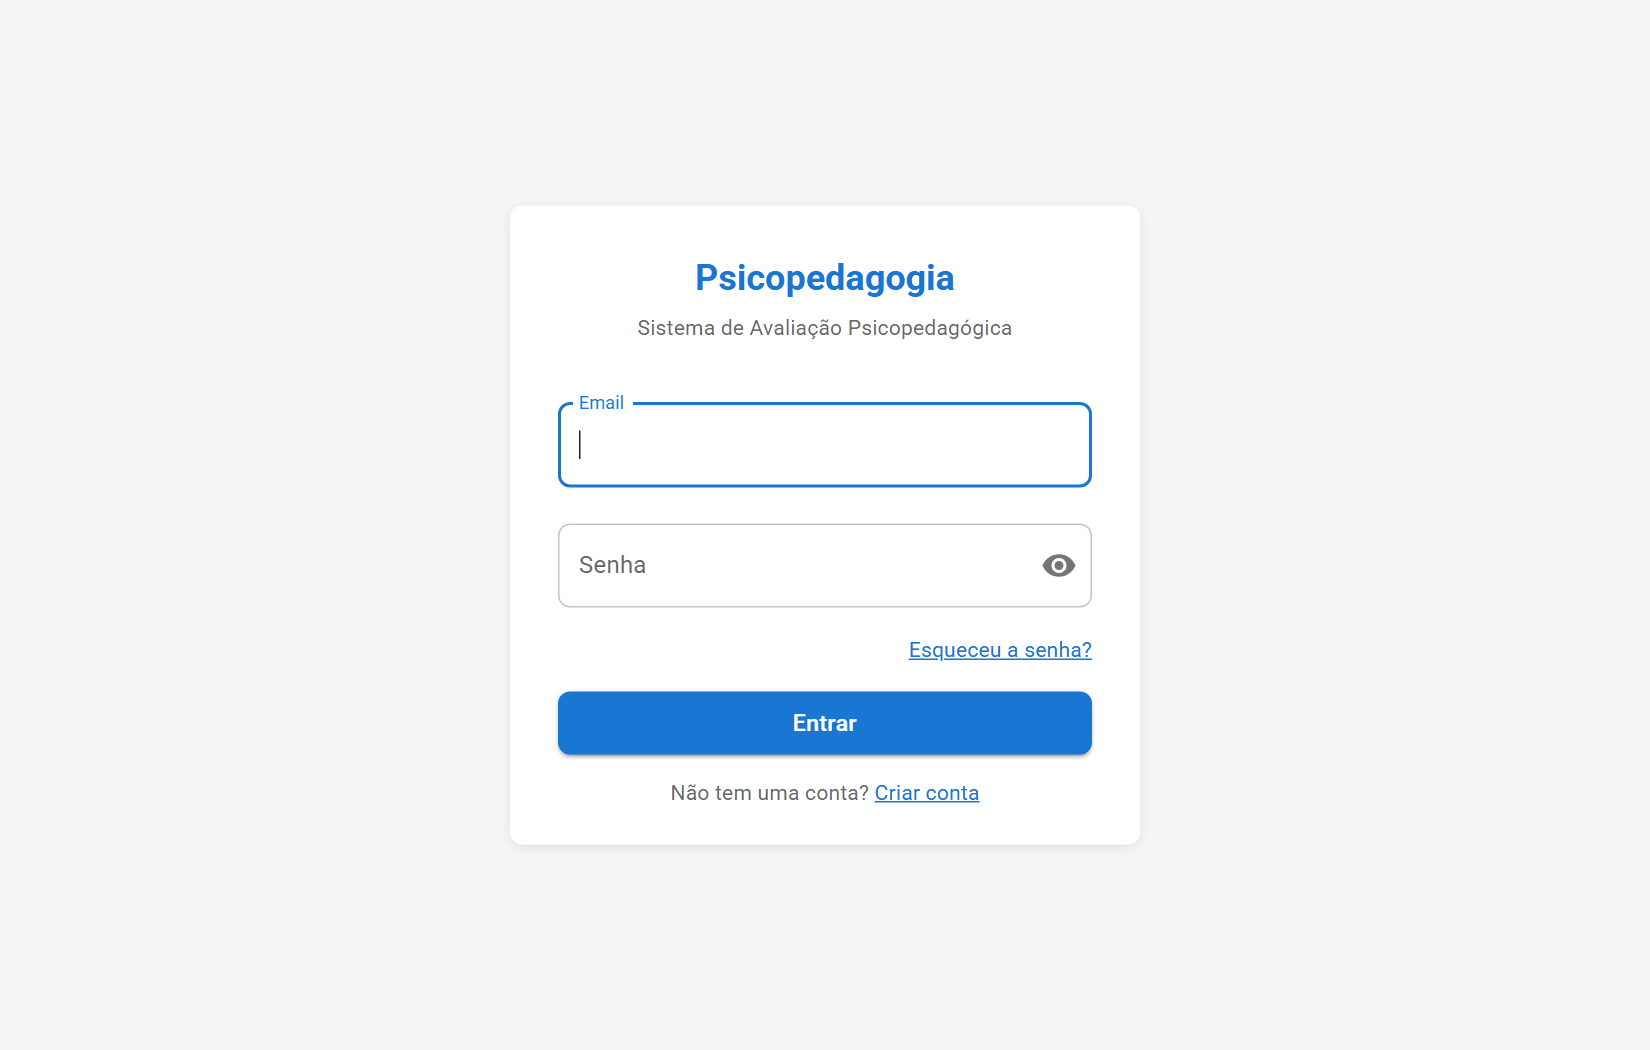
\includegraphics[width=0.70\textwidth]{tela_login.png}
    \fonte{Elaborado pela autora (2026).}
\end{figure}

Após a autenticação, o usuário é direcionado ao \textit{dashboard} (Figura~\ref{fig:tela_dashboard}). A estrutura da tela se repete nas demais páginas autenticadas: a barra superior e o menu lateral são fornecidos pelo componente \textit{AppLayout}. Os indicadores mostram os totais de aprendentes, de instrumentos ativos e de aplicações, além das aplicações mais recentes com o respectivo status, considerando apenas os registros do profissional autenticado.

\begin{figure}[H]
    \centering
    \caption{\textit{Dashboard} do perfil psicopedagogo}
    \label{fig:tela_dashboard}
    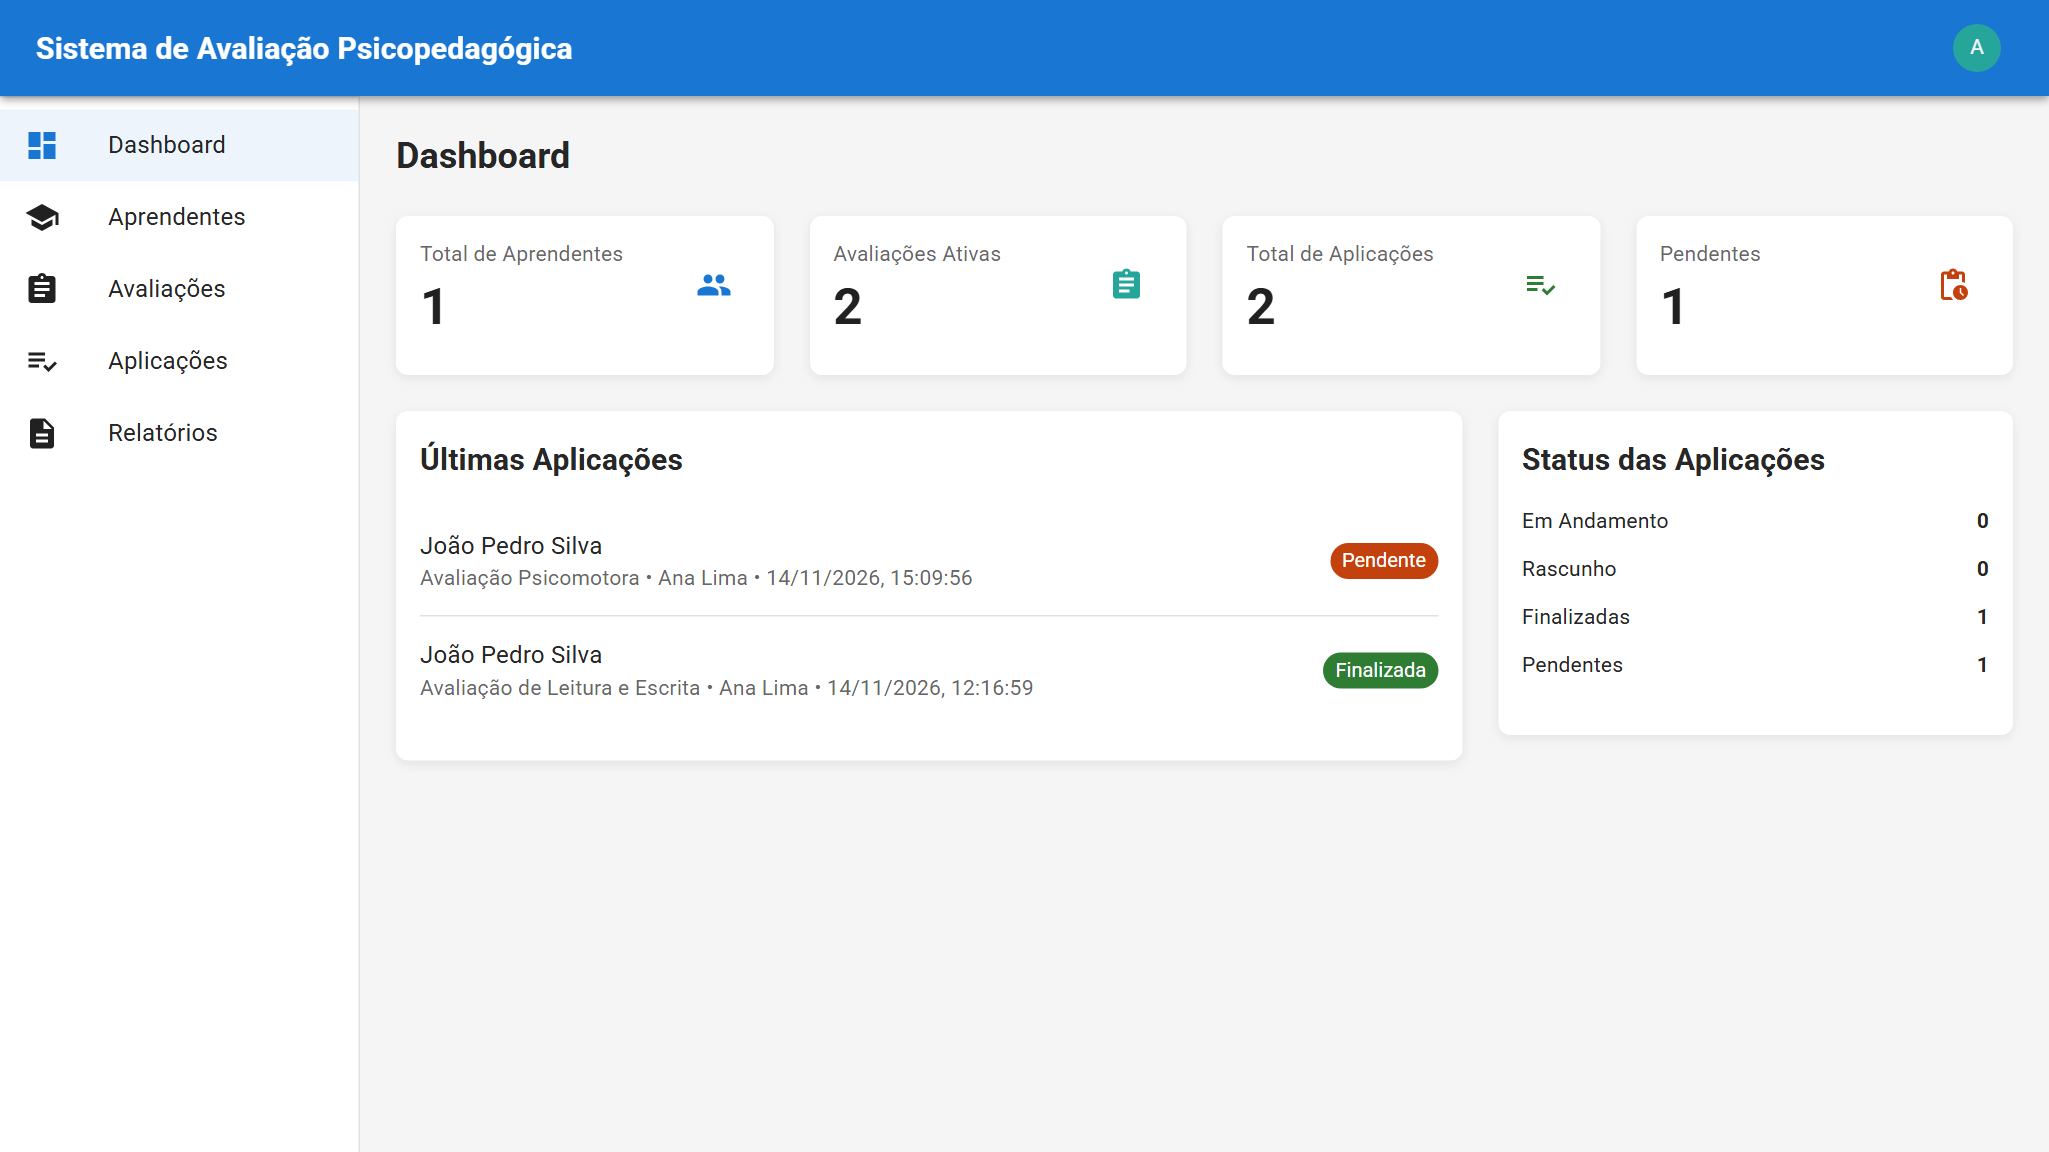
\includegraphics[width=\textwidth]{tela_dashboard.png}
    \fonte{Elaborado pela autora (2026).}
\end{figure}

O cadastro de aprendentes (Figura~\ref{fig:tela_aprendente_form}) organiza os campos em três grupos: dados do aprendente, dados do responsável e dados escolares. Os campos obrigatórios são marcados com asterisco e validados pelo mesmo esquema Zod do \textit{backend}, compartilhado entre as duas aplicações pelo pacote \textit{shared-validation}. O mesmo formulário é utilizado para cadastro e edição; na edição, os campos são preenchidos com os dados atuais do registro.

\begin{figure}[H]
    \centering
    \caption{Formulário de cadastro e edição de aprendente}
    \label{fig:tela_aprendente_form}
    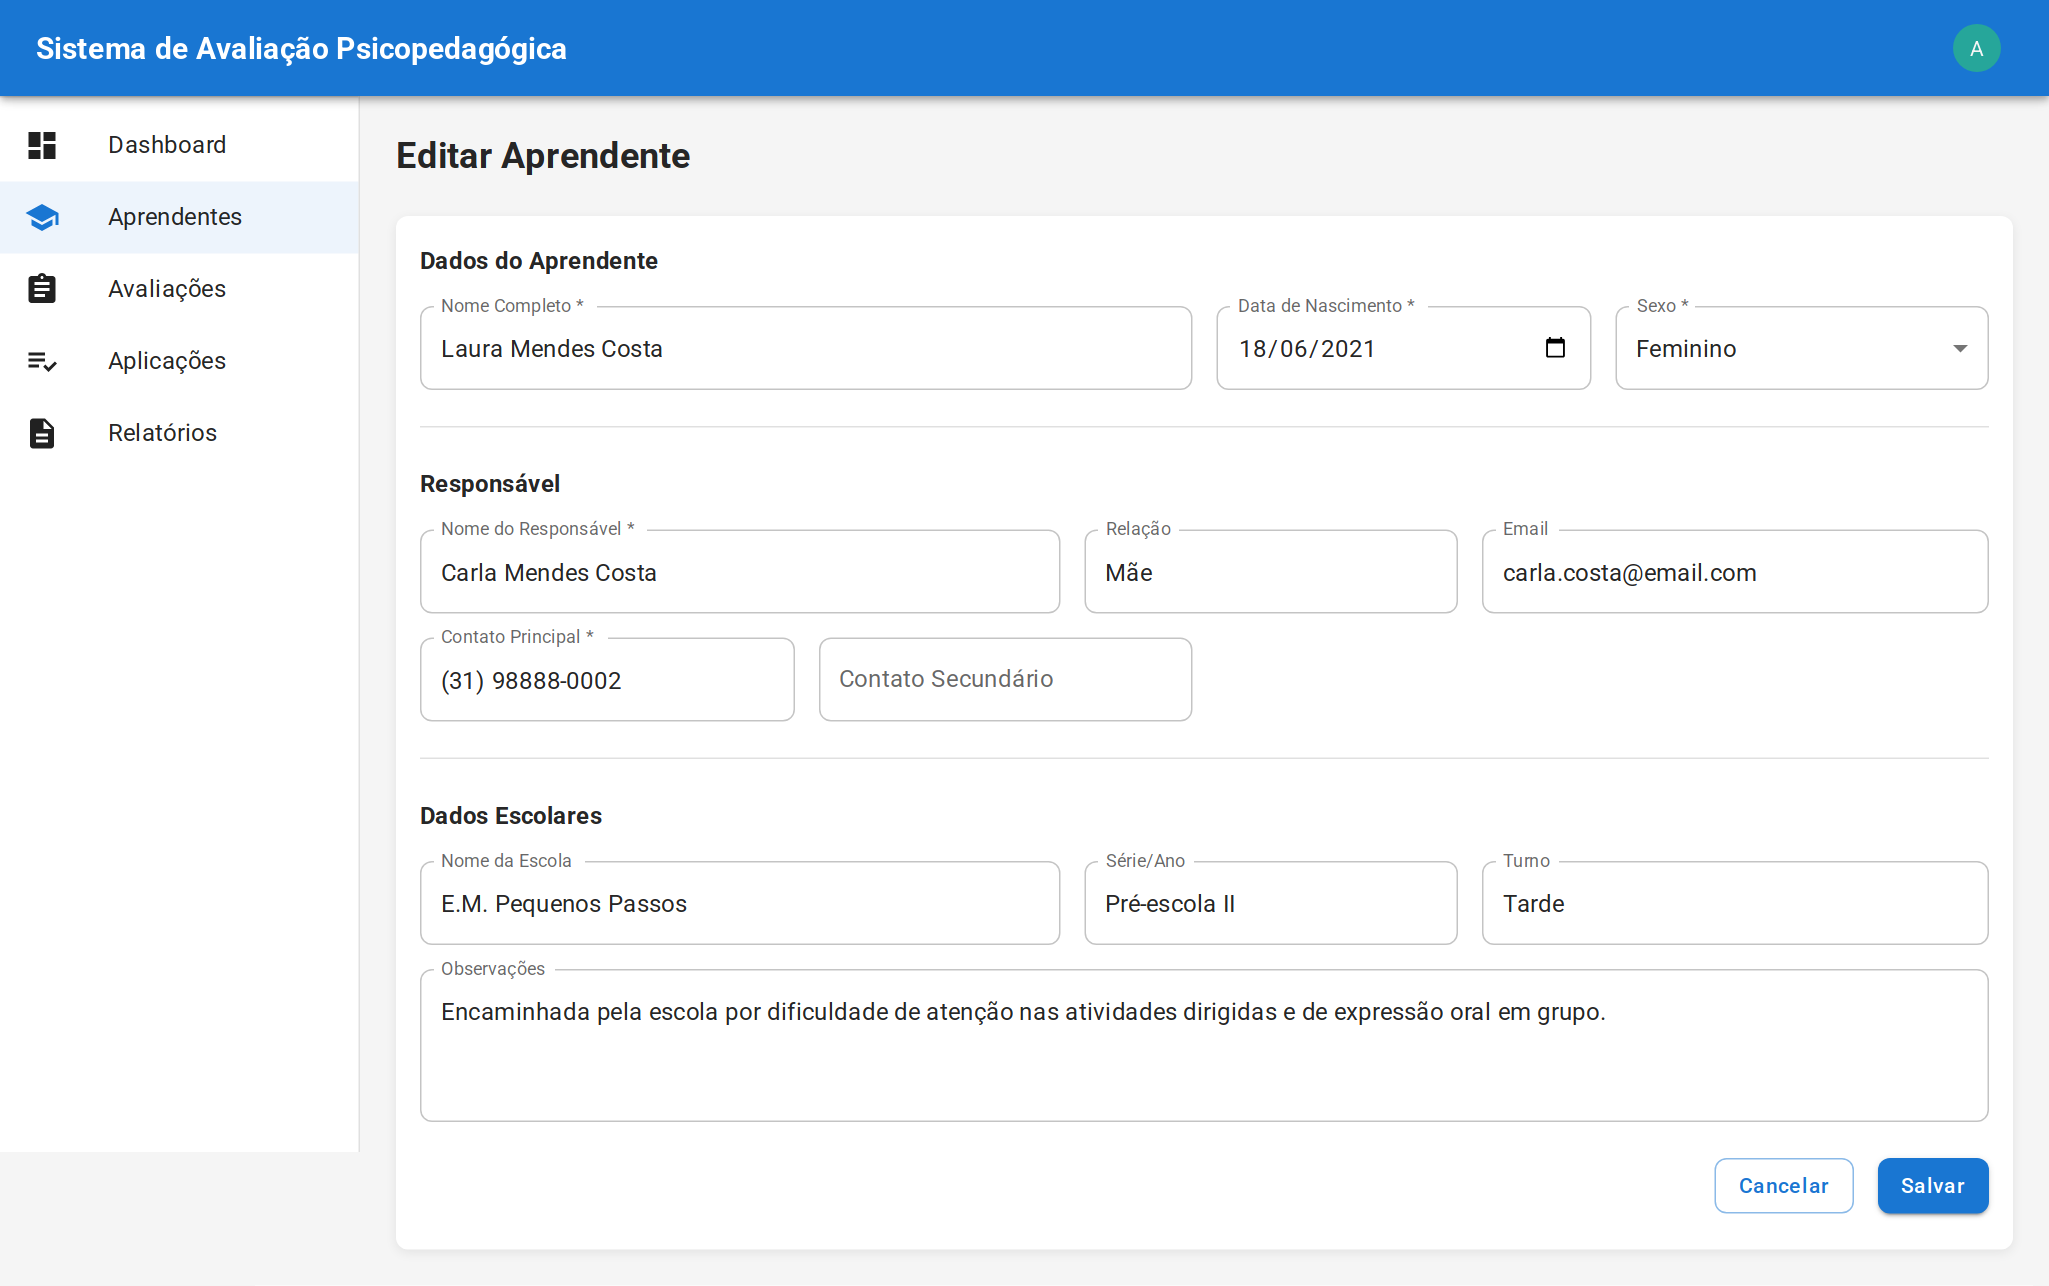
\includegraphics[width=\textwidth]{tela_aprendente_form.png}
    \fonte{Elaborado pela autora (2026).}
\end{figure}

A página de detalhe do aprendente (Figura~\ref{fig:tela_aprendente_detalhe}) reúne, em abas, os dados cadastrais, o histórico de acompanhamento e o registro de acessos.

\begin{figure}[H]
    \centering
    \caption{Página de detalhe do aprendente, com as abas de dados cadastrais, histórico e registro de acessos}
    \label{fig:tela_aprendente_detalhe}
    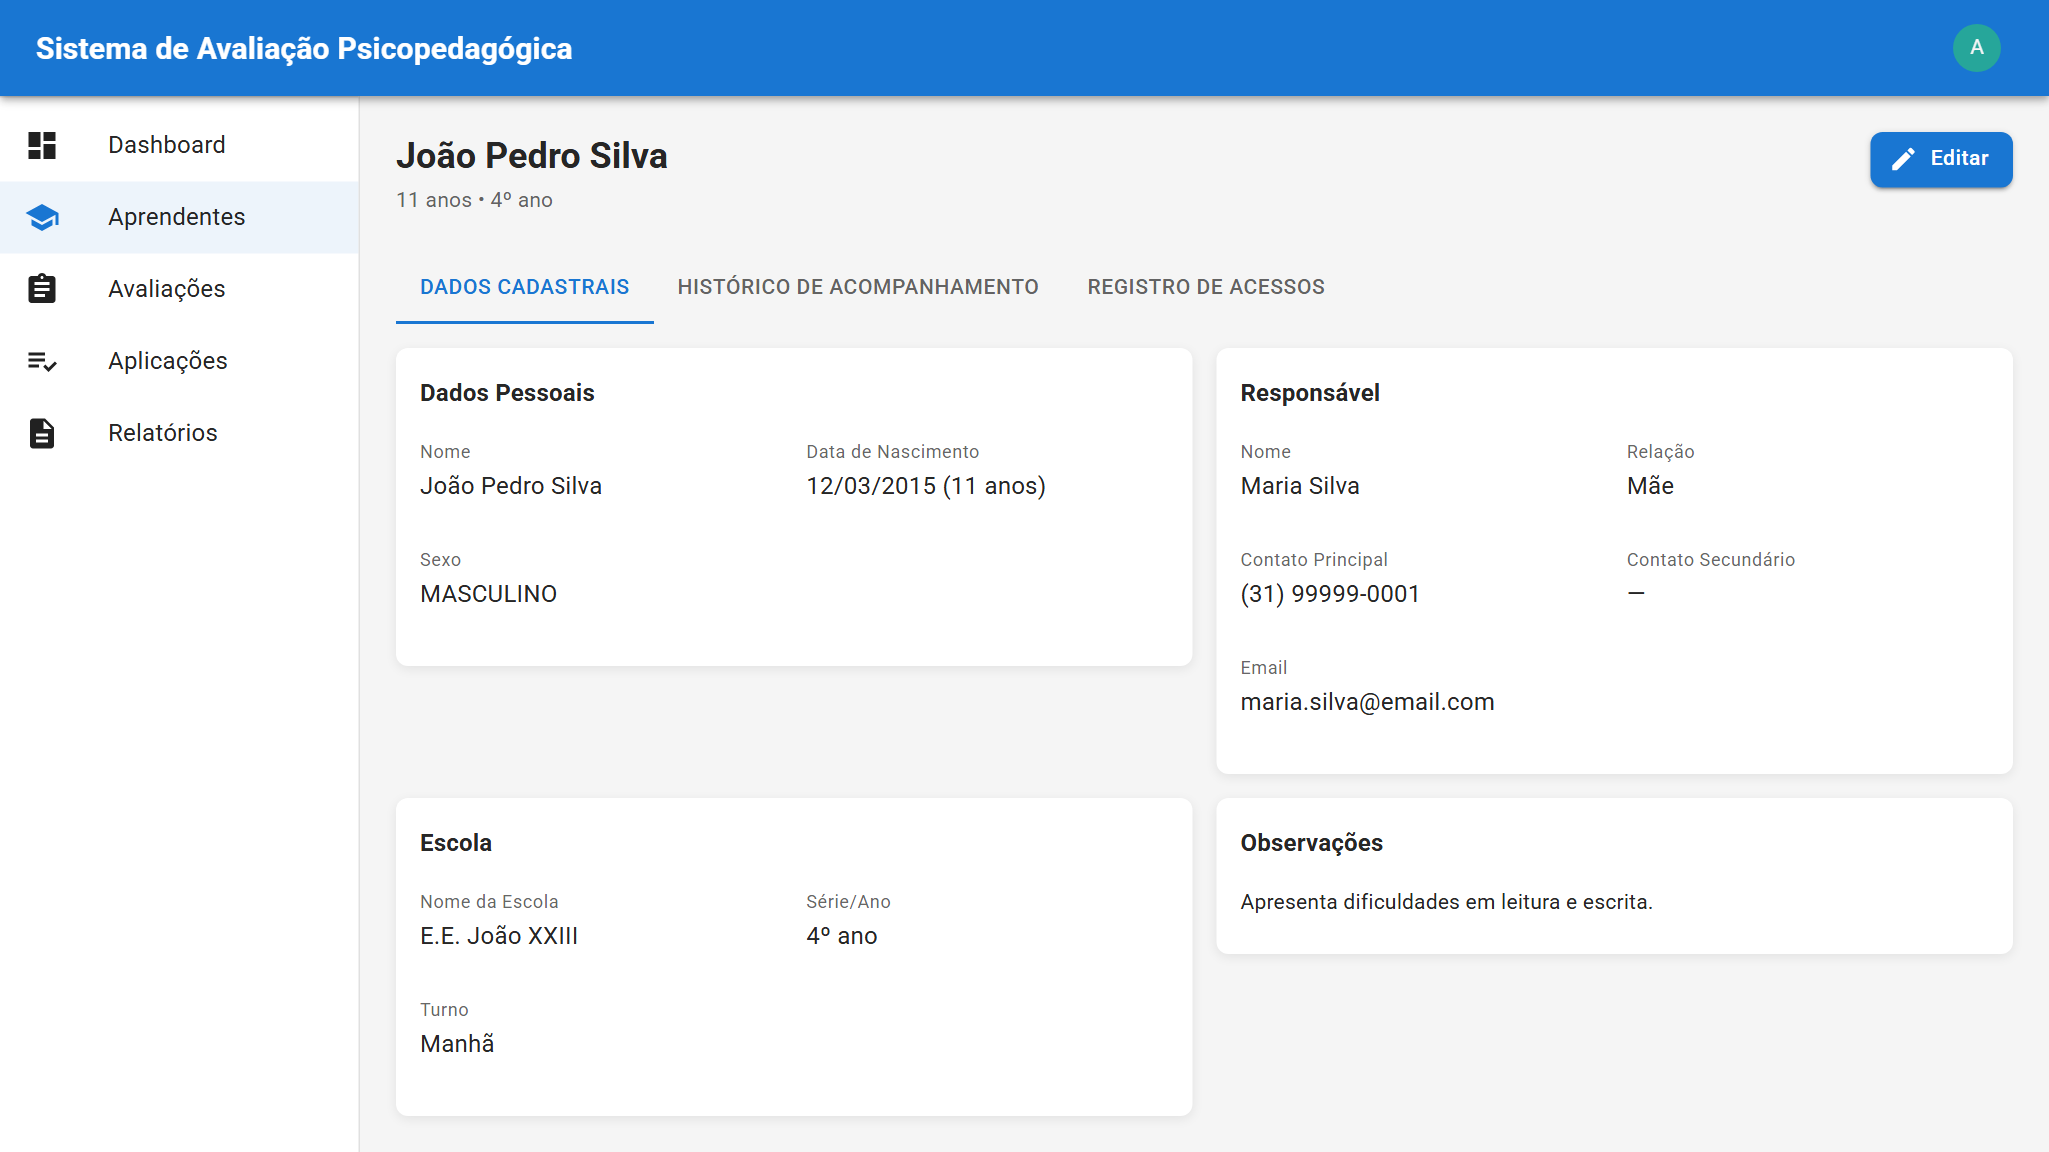
\includegraphics[width=\textwidth]{tela_aprendente_detalhe.png}
    \fonte{Elaborado pela autora (2026).}
\end{figure}

O editor de instrumentos (Figura~\ref{fig:tela_instrumento_editor}) permite definir o nome, a categoria, a descrição e o status do instrumento e compor sua lista de perguntas. Para cada pergunta são escolhidos o tipo de resposta e a obrigatoriedade; os campos complementares variam conforme o tipo, como os limites e rótulos de uma escala, mostrados na pergunta 2, ou as opções de uma questão de múltipla escolha. Quando o instrumento já foi aplicado, um aviso no topo da tela informa que a alteração das perguntas criará uma nova versão, mecanismo detalhado na Seção~\ref{sec:instrumentos}.

\begin{figure}[H]
    \centering
    \caption{Editor de instrumento avaliativo, com o aviso de criação de nova versão}
    \label{fig:tela_instrumento_editor}
    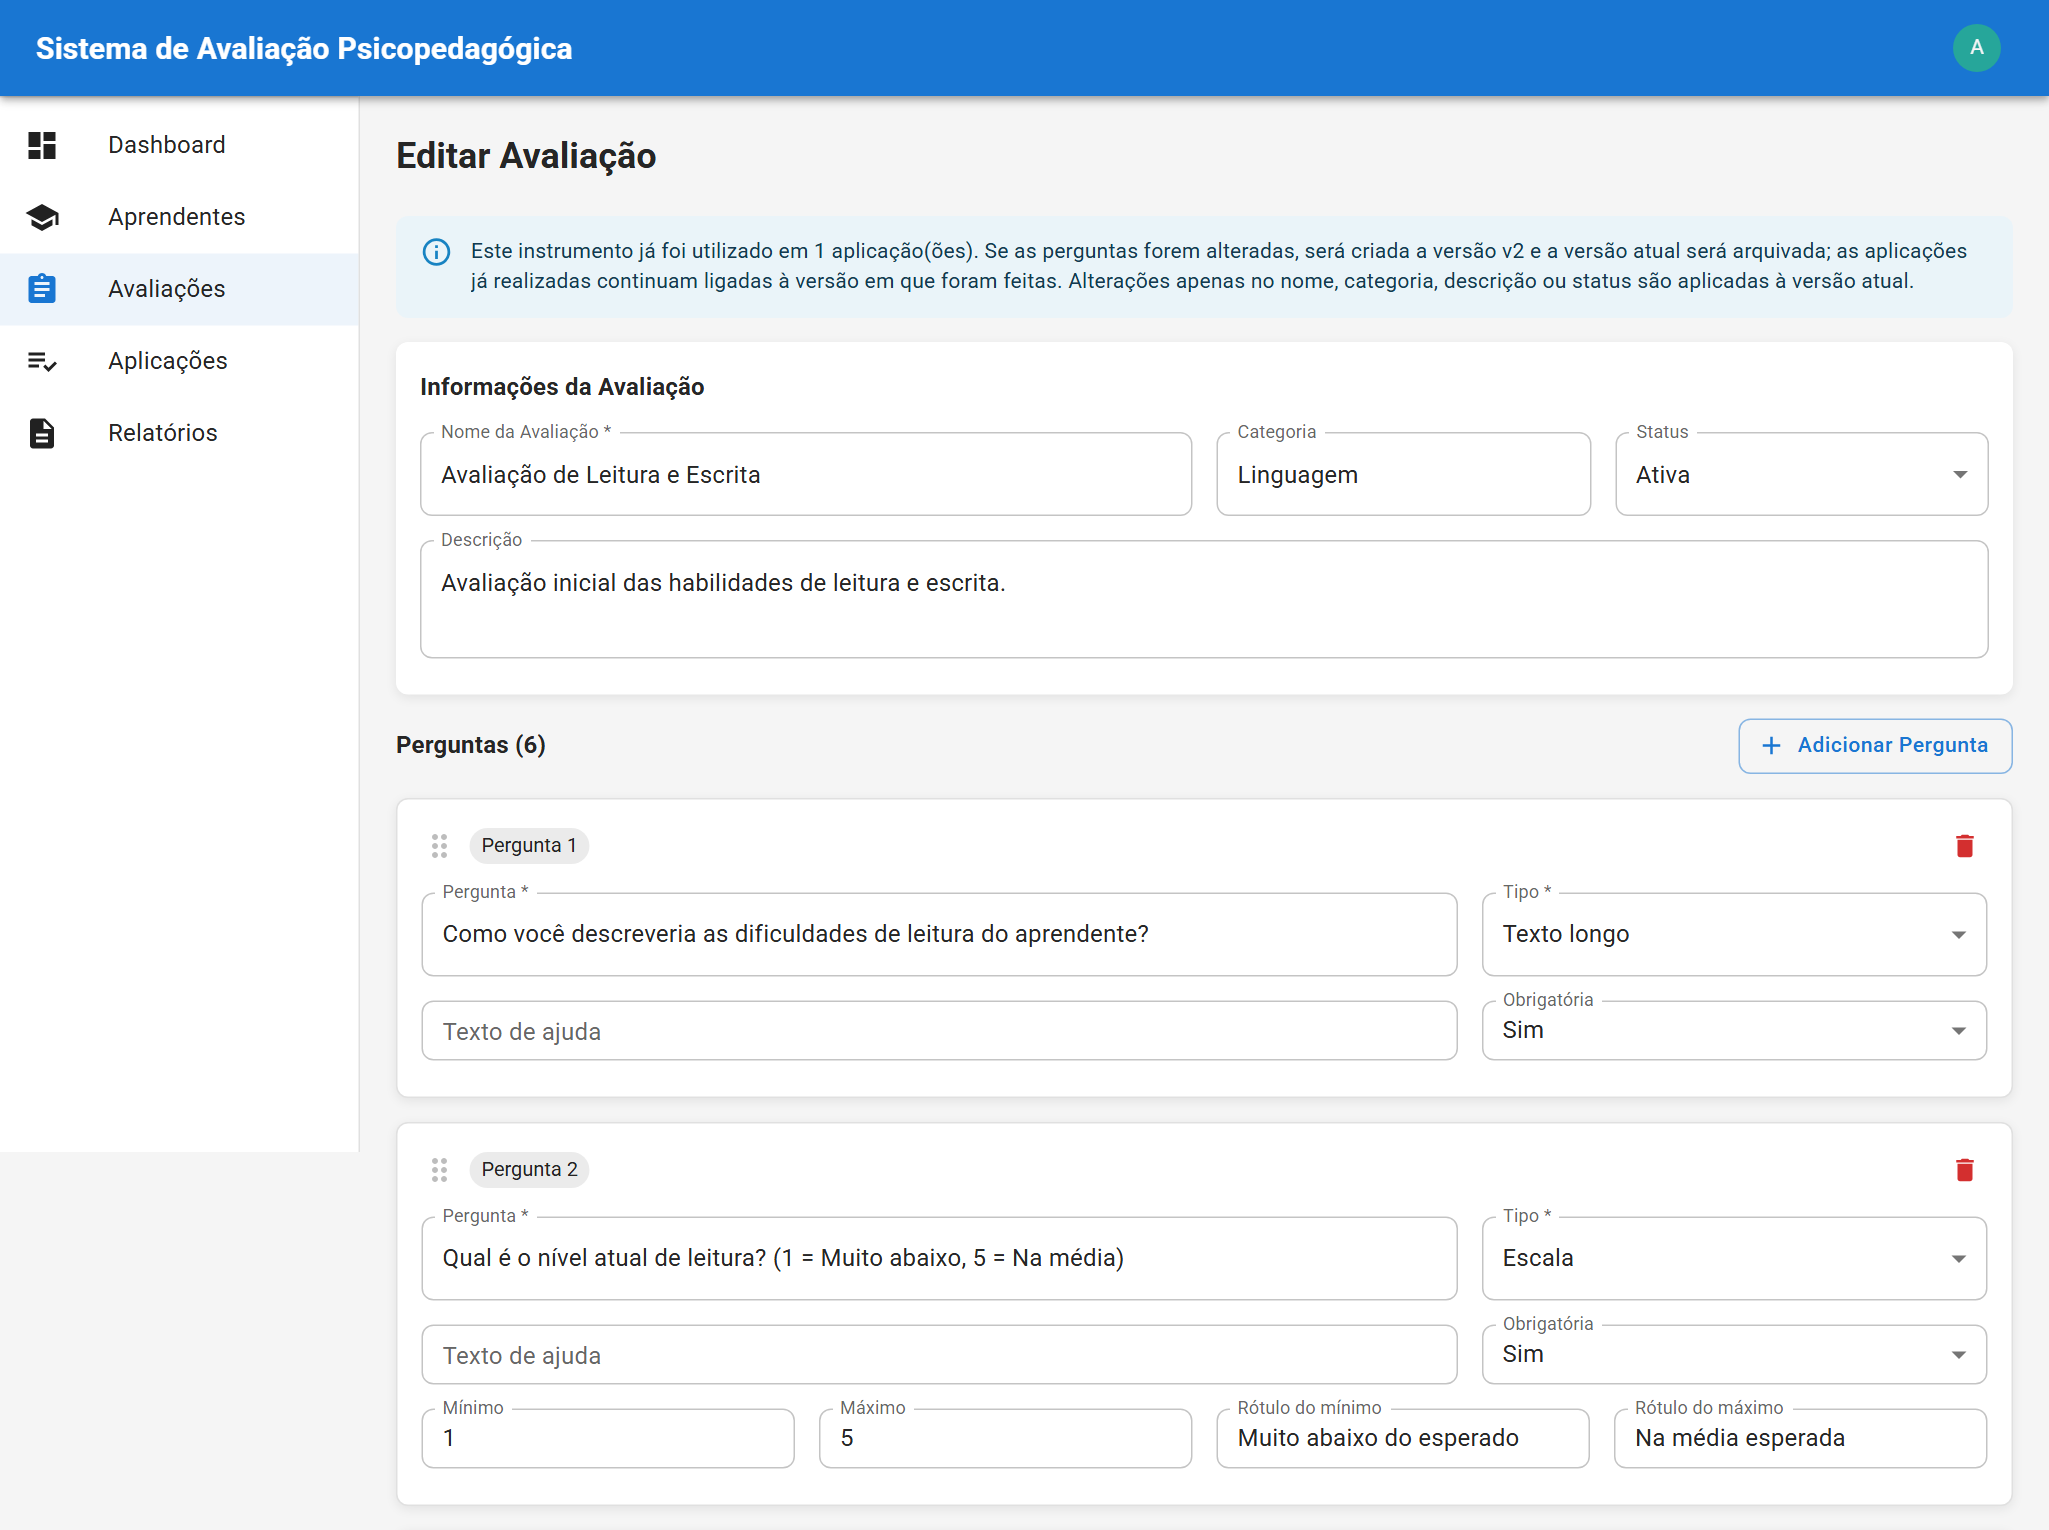
\includegraphics[width=\textwidth]{tela_instrumento_editor.png}
    \fonte{Elaborado pela autora (2026).}
\end{figure}

A Figura~\ref{fig:tela_aplicacao} mostra a tela de aplicação de um instrumento a um aprendente. Cada pergunta é apresentada com o componente de entrada correspondente ao seu tipo: campo de texto, botões de opção, sim/não ou campo numérico. Os três botões ao final correspondem aos estados da aplicação: as respostas podem ser salvas como rascunho ou como progresso normal e retomadas depois, e a finalização verifica o preenchimento das perguntas obrigatórias e bloqueia a edição das respostas, conforme descrito na Seção~\ref{sec:aplicacoes}.

\begin{figure}[H]
    \centering
    \caption{Tela de aplicação de um instrumento, com perguntas de tipos diferentes}
    \label{fig:tela_aplicacao}
    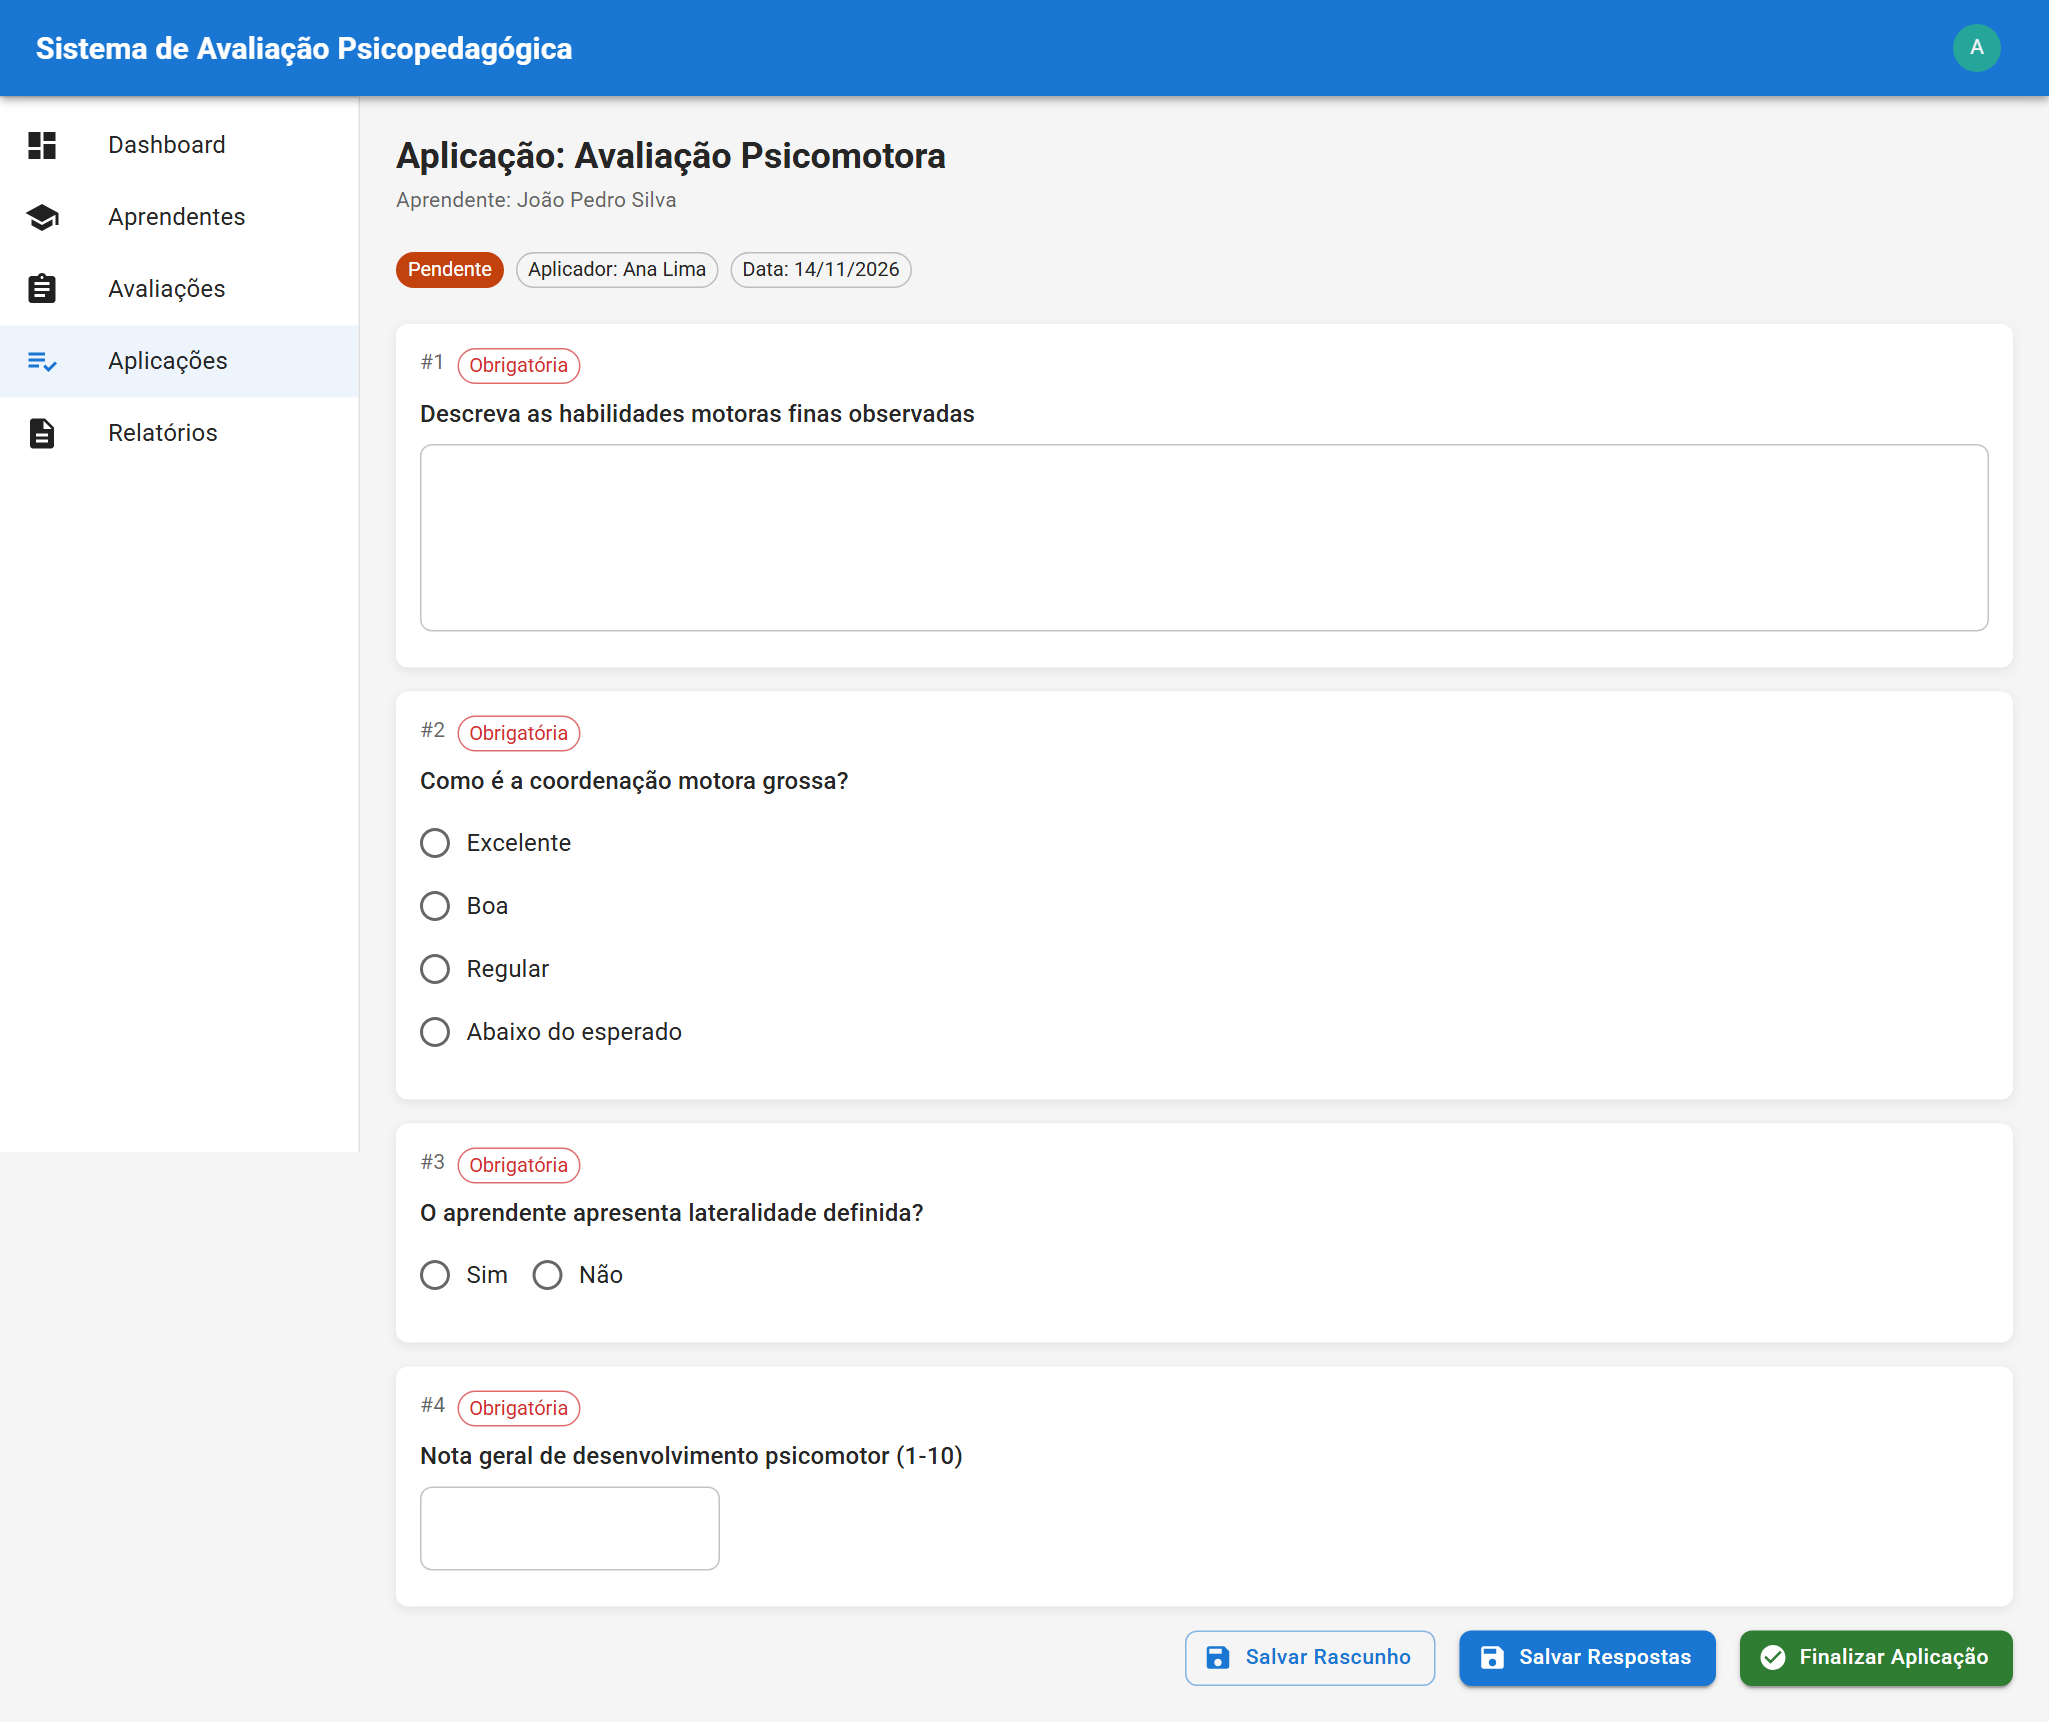
\includegraphics[width=\textwidth]{tela_aplicacao.png}
    \fonte{Elaborado pela autora (2026).}
\end{figure}

Por fim, a Figura~\ref{fig:tela_relatorio_impresso} apresenta o relatório na forma em que é impresso ou exportado em PDF pelo navegador. A folha de estilos de impressão oculta o menu, a barra superior e os botões, e o documento reúne os dados do aprendente, a identificação do instrumento e de sua versão, as respostas registradas, as observações e a conclusão do profissional, seguidas do espaço para assinatura. A organização desse documento é discutida na Seção~\ref{sec:relatorios}.

\begin{figure}[H]
    \centering
    \caption{Relatório de avaliação psicopedagógica no formato de impressão}
    \label{fig:tela_relatorio_impresso}
    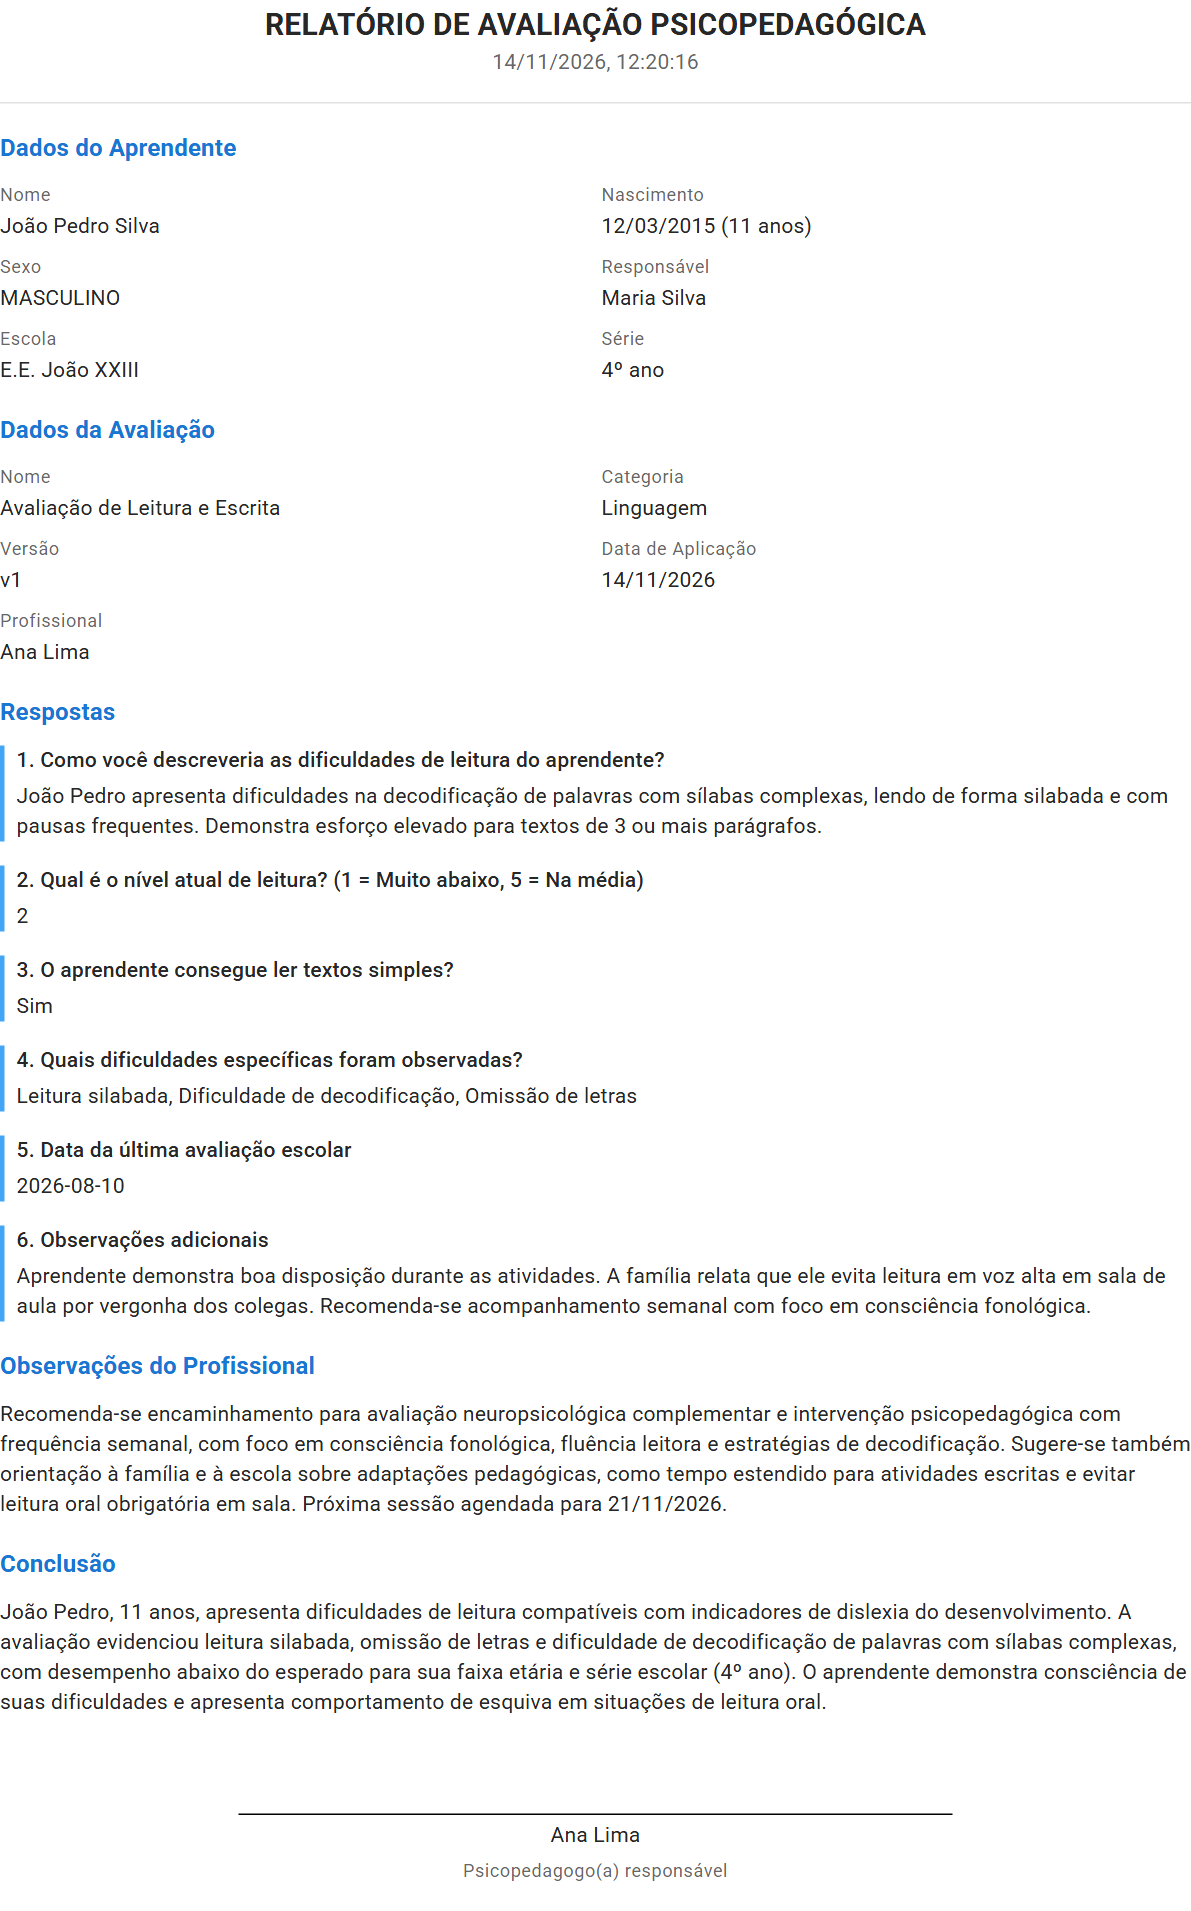
\includegraphics[width=0.85\textwidth,height=0.80\textheight,keepaspectratio]{tela_relatorio_impresso.png}
    \fonte{Elaborado pela autora (2026).}
\end{figure}

\subsection{Testes do \textit{frontend}}

Os testes do \textit{frontend} utilizam o Vitest e a React Testing Library, que renderiza os componentes em ambiente simulado (jsdom) e permite interagir com eles como um usuário faria, sem navegador real. Assim como no \textit{backend}, as chamadas à API são simuladas. Foram implementados 59 testes em 11 arquivos, concentrados nas páginas e componentes com mais lógica de apresentação, conforme o Quadro~\ref{qua:testes_frontend}.

\begin{quadro}[H]
\centering
\footnotesize
\caption{Distribuição dos testes automatizados do \textit{frontend}}
\begin{tabular}{|p{5.2cm}|c|p{7.6cm}|}
\hline
\textbf{Arquivo de teste} & \textbf{Testes} & \textbf{Escopo} \\ \hline
LoginPage.test.jsx & 6 & Formulário de \textit{login}, validações e nome acessível do botão de senha \\ \hline
ProtectedRoute.test.jsx & 6 & Redirecionamento por autenticação e perfil, inclusive do administrador nas rotas clínicas \\ \hline
AvaliacaoFormPage.test.jsx & 8 & Formulário de criação e edição de instrumento \\ \hline
AvaliacaoDetailPage.test.jsx & 6 & Exibição do instrumento e ausência da edição para o administrador \\ \hline
AplicacaoDetailPage.test.jsx & 9 & Preenchimento e finalização de aplicação \\ \hline
Auditoria.test.jsx & 6 & Listagem, filtros e aviso de valores clínicos omitidos \\ \hline
RelatorioDetailPage.test.jsx & 7 & Exibição e edição de relatório, inclusive a formatação das respostas \\ \hline
DashboardPage.test.jsx & 2 & \textit{Dashboard} do administrador (só totais) e do psicopedagogo \\ \hline
UsersListPage.test.jsx & 2 & Transferência de aprendentes entre profissionais \\ \hline
StatusChip.test.jsx & 4 & Componente de status e suas variações visuais \\ \hline
print.test.jsx & 3 & Função utilitária de impressão/PDF \\ \hline
\textbf{Total} & \textbf{59} & \\ \hline
\end{tabular}
\fonte{Elaborado pela autora (2026).}
\label{qua:testes_frontend}
\end{quadro}

A cobertura de linhas do \textit{frontend} foi de 55,87\%. O valor é menor que o do \textit{backend} porque várias telas não têm testes próprios, como as listagens, o formulário e a página de detalhe do aprendente e as telas de autocadastro e de recuperação de senha. Os testes priorizaram os fluxos de maior risco: autenticação, controle de acesso por perfil, preenchimento e finalização das aplicações e relatórios. Não foi definido critério mínimo de cobertura para o \textit{frontend}.


\section{Funcionalidades do processo avaliativo}\label{sec:funcionalidades}

As funcionalidades centrais do sistema acompanham o percurso de uma avaliação: o profissional cadastra e, quando necessário, adapta um instrumento; aplica-o a um aprendente, registrando as respostas; e, ao final, elabora o relatório. Esta seção descreve cada uma dessas etapas, cuja estrutura de dados foi apresentada na Seção~\ref{sec:modelagem}.

\subsection{Gerenciamento e versionamento dos instrumentos}\label{sec:instrumentos}

Para criar um instrumento, o profissional acessa o módulo de instrumentos e cria um novo instrumento informando nome, categoria e descrição. Em seguida, adiciona as questões, definindo para cada uma o texto, o tipo de resposta, a obrigatoriedade e a ordem de apresentação. O instrumento é criado com estado \textit{DRAFT} e só fica disponível para aplicação após ser explicitamente ativado (\textit{ACTIVE}).

Enquanto o instrumento não foi usado em nenhuma aplicação, todas as edições, inclusive a adição, a remoção e a alteração de questões, são salvas no próprio registro, sem gerar nova versão. Quando o profissional tenta editar as questões de um instrumento que já possui ao menos uma aplicação vinculada, a interface exibe um aviso informando que a alteração criará uma nova versão. Ao confirmar, o sistema arquiva o registro atual (estado \textit{ARCHIVED}) e cria automaticamente um novo registro com versão incrementada, herdando os metadados e recebendo as novas questões. O registro anterior permanece intacto e continua associado a todas as aplicações já realizadas com ele.

Alterações apenas no nome, na categoria, na descrição ou no status não geram nova versão; são aplicadas ao registro existente e ficam documentadas na auditoria, com os valores anteriores e os novos. A tela do instrumento mostra a versão de origem e as versões derivadas, o que permite navegar pelo histórico. Como cada aplicação guarda uma referência direta à versão utilizada, alterações posteriores nunca modificam retroativamente o histórico do aprendente.

O sistema não oferece, contudo, um campo para que o profissional registre a justificativa de cada adaptação. Essa informação fica registrada apenas de forma estrutural (número da versão, data e usuário, na auditoria), o que é uma limitação da implementação atual; a motivação precisa ser anotada por outros meios, como o histórico do aprendente.

Quanto à titularidade, ao criar uma nova versão o sistema atribui como autor o usuário que realizou a alteração. Como a edição de instrumentos é exclusiva do perfil \textit{PSICOPEDAGOGO} e cada profissional só edita os instrumentos que criou, o autor da nova versão é sempre o próprio autor do instrumento, e a titularidade se mantém entre as versões.

Ressalta-se que o versionamento registra e organiza as versões, mas não realiza a validação metodológica de uma adaptação, cuja adequação permanece sob responsabilidade do profissional.

\subsection{Aplicação dos instrumentos}\label{sec:aplicacoes}

A aplicação relaciona um instrumento a um aprendente e registra as respostas obtidas no atendimento. Seu andamento é representado por quatro estados: \textit{PENDING} (criada, sem respostas registradas), \textit{IN\_PROGRESS} (respostas salvas em modo de progresso normal), \textit{DRAFT} (respostas salvas explicitamente como rascunho pelo profissional, sinalizando preenchimento pausado intencionalmente) e \textit{COMPLETED} (finalizada). Os estados \textit{IN\_PROGRESS} e \textit{DRAFT} têm o mesmo comportamento, pois ambos guardam as respostas e permitem retomar o preenchimento depois. A diferença é apenas de sinalização: ao salvar como rascunho, o profissional indica que pausou a aplicação de propósito, por exemplo para continuar em outra sessão, e essa informação aparece nas listagens. Os testes com usuários não avaliaram se essa distinção é clara para os profissionais, ponto que pode ser simplificado em versões futuras.

A partir de qualquer estado não finalizado, o profissional pode concluir a aplicação. Nesse momento, o sistema verifica o preenchimento das questões obrigatórias, e as respostas ficam bloqueadas para edição; aplicações finalizadas também não podem ser excluídas. O formulário de preenchimento é construído a partir da configuração das questões do instrumento, apresentando para cada uma o componente de entrada correspondente ao seu tipo.

Separar o instrumento de suas aplicações preserva o histórico: o instrumento é uma estrutura reutilizável, e cada aplicação é uma ocorrência específica, associada à versão empregada (Seção~\ref{sec:instrumentos}). Assim, um mesmo aprendente pode ter várias aplicações em momentos diferentes, cada uma com seus próprios registros.


\subsection{Geração dos relatórios}\label{sec:relatorios}

O relatório é elaborado após a finalização de uma aplicação e documenta as considerações do profissional a partir das informações obtidas no processo avaliativo. Cada relatório pertence a uma única aplicação (Seção~\ref{sec:modelagem}) e, por meio dela, fica contextualizado: identifica o aprendente, o instrumento e sua versão, o profissional, a data e as respostas registradas, de modo que a devolutiva não é tratada como um registro isolado.

Os campos destinados ao conteúdo do relatório são \textit{conclusao}, que registra a síntese elaborada pelo profissional, e \textit{observacoesProfissional}, que permite acrescentar informações complementares. As respostas dos instrumentos permanecem na entidade \textit{respostas}, separadas da interpretação registrada no relatório. Essa separação é deliberada: o sistema não converte os resultados de uma avaliação em diagnósticos ou conclusões psicopedagógicas, e a análise e a interpretação permanecem atribuições do profissional responsável pelo atendimento.

A página do relatório tem uma função de impressão, que abre o diálogo do navegador e permite imprimir o documento ou salvá-lo em PDF. Uma folha de estilos aplicada apenas na impressão configura a página em A4, oculta o cabeçalho, o menu lateral e os botões, imprime as observações e a conclusão como texto corrido, mantém cada pergunta e sua resposta na mesma página e encerra o documento com um espaço para a assinatura do profissional. A geração do PDF, portanto, usa a capacidade nativa do navegador, sem bibliotecas no servidor.

O documento inclui, na seção ``Dados da Avaliação'', o nome, a categoria e a versão do instrumento (por exemplo, ``v1''), como mostra a Figura~\ref{fig:tela_relatorio_impresso}. Como cada aplicação aponta para a versão do instrumento efetivamente utilizada, e não para a mais recente, o documento continua identificando corretamente o protocolo vigente no momento da avaliação mesmo após adaptações posteriores do instrumento.


\section{Segurança e controle de acesso}\label{sec:seguranca}

Os mecanismos de autenticação, autorização e validação foram descritos nas Seções~\ref{sec:backend} e~\ref{sec:frontend}. Esta seção discute o que eles garantem, a rastreabilidade das operações e as limitações para o uso com dados reais.

Todas as decisões de acesso são tomadas no \textit{backend}, onde os dois controles se complementam. O perfil (RBAC) separa a administração do sistema do atendimento, pelas razões discutidas na Seção~\ref{sec:separacao_admin}, e a titularidade garante que psicopedagogos distintos não acessem os registros uns dos outros, mesmo tendo o mesmo perfil. Registros de outros profissionais são tratados como inexistentes, sem revelar que existem, e a criação de uma aplicação exige que o aprendente e o instrumento pertençam ao próprio profissional. O campo \textit{status} da entidade \textit{users} permite ainda desativar uma conta, que deixa de ser aceita na validação de cada requisição.

No cadastro, na redefinição e na alteração de senha, o \textit{backend} gera um \textit{hash} com o algoritmo bcrypt, utilizando fator de custo 12, e somente esse \textit{hash} é gravado no campo \textit{passwordHash} da entidade \textit{users}. Na autenticação, a senha informada é comparada ao \textit{hash} armazenado, sem que a senha original precise ser recuperada.

Quanto à rastreabilidade, os campos de data (\textit{createdAt} e \textit{updatedAt}) e de autoria (\textit{responsavelId}, \textit{autorId} e \textit{aplicadorId}) não bastam para dados de saúde de crianças: indicam quem criou cada registro e quando ele foi alterado pela última vez, mas não quem fez cada alteração, quais eram os valores anteriores nem quem consultou as informações, que é justamente o que a LGPD e o sigilo profissional mais exigem. Por isso, o sistema mantém o registro de auditoria descrito na Seção~\ref{sec:auditoria}, que identifica o autor de cada operação, guarda os valores anteriores, associa as consultas a dados clínicos ao aprendente e registra as operações do administrador, como a transferência de responsabilidade. Esse registro apresenta, entretanto, as seguintes limitações:

\begin{itemize}
    \item o registro é gravado após a operação, em uma conexão separada, e não faz parte da mesma transação. Se a gravação da auditoria falhar, a operação é mantida e a falha aparece apenas no \textit{log} do servidor. Em operações executadas dentro de uma transação, o registro pode permanecer mesmo que a transação seja desfeita;
    \item não há garantia de imutabilidade. A aplicação não oferece meios de alterar ou excluir o registro, mas quem tem acesso direto ao banco de dados pode modificá-lo, pois não há encadeamento criptográfico dos registros nem armazenamento externo somente de gravação;
    \item acessos feitos diretamente ao banco de dados ou às suas cópias de segurança não passam pela aplicação e, portanto, não são registrados;
    \item o próprio registro contém dados sensíveis, pois guarda valores anteriores e novos dos dados clínicos. Por isso, a consulta geral é restrita ao administrador, que recebe apenas os metadados dos registros clínicos, mas não foi definida uma política de retenção e descarte desses registros;
    \item as consultas do administrador ao próprio registro de auditoria não são registradas;
    \item as leituras feitas internamente pelo sistema, como a verificação de permissão antes de uma alteração, também são registradas como consultas, e as listagens geram um registro por item exibido. Isso aumenta o volume de registros e pode dificultar a análise. Contagens agregadas, como as do \textit{dashboard}, não são registradas, assim como as tentativas de acesso negadas a registros de outros profissionais;
    \item o endereço IP registrado depende da configuração do \textit{proxy} reverso. Se a API estiver acessível diretamente, sem passar pelo \textit{proxy}, o cabeçalho que informa o IP de origem pode ser falsificado.
\end{itemize}

Trata-se, portanto, de um mecanismo básico de rastreabilidade, compatível com o estágio de protótipo.

\subsection{Separação entre administração e acesso aos dados clínicos}\label{sec:separacao_admin}

Na primeira versão do sistema, o perfil \textit{ADMIN} tinha acesso irrestrito a todos os registros, inclusive às avaliações e aos relatórios das crianças, seguindo o padrão comum de tratar o administrador como superusuário. Essa escolha reunia em um mesmo perfil duas atribuições distintas, a gestão técnica do sistema e o atendimento psicopedagógico, e quem cadastra contas não é necessariamente o profissional responsável pelas crianças.

Do ponto de vista do sigilo profissional, esse acesso não se justifica. O Código de Ética do Psicopedagogo determina que o profissional mantenha o sigilo e preserve a confidencialidade dos dados obtidos no exercício da atividade (art. 7º) e estabelece que os registros de atendimento psicopedagógico são documentos sigilosos cujo acesso é restrito ao psicopedagogo responsável (art. 9º); o compartilhamento com outros especialistas só deixa de constituir quebra de sigilo quando autorizado pelos próprios atendidos ou por seus responsáveis legais (art. 7º, §1º) \cite{abpp2019_codigo_etica}. Um sistema que concede a um terceiro acesso irrestrito a esses registros faz, pelo \textit{software}, o compartilhamento que o próprio profissional não poderia fazer sem autorização. A LGPD aponta na mesma direção: o princípio da necessidade limita o tratamento ao mínimo necessário para suas finalidades (art. 6º, III), e os agentes de tratamento devem adotar medidas de segurança aptas a proteger os dados de acessos não autorizados (art. 46) \cite{brasil2018_lgpd}. Administrar contas de usuário não exige ler a avaliação de uma criança. Em termos de projeto de sistemas, trata-se do princípio do menor privilégio, segundo o qual cada usuário deve operar com o mínimo de privilégios necessário para realizar sua tarefa \cite{saltzer1975_protection}.

Por esses motivos, a administração de usuários foi separada do acesso aos dados clínicos:

\begin{itemize}
    \item as rotas de aprendentes, histórico de acompanhamento, aplicações e relatórios exigem o perfil \textit{PSICOPEDAGOGO} em todas as operações, inclusive nas de leitura, e respondem HTTP 403 ao administrador antes de qualquer consulta ao banco de dados. O filtro de titularidade deixou de ter exceção por perfil e funciona como segunda barreira;
    \item o \textit{dashboard} do administrador apresenta apenas contagens agregadas, sem a lista das últimas aplicações, que identifica as crianças atendidas;
    \item no registro de auditoria, o administrador continua consultando quem realizou cada operação, quando e de onde, mas os valores dos registros clínicos não lhe são enviados, apenas os nomes dos campos alterados. O psicopedagogo responsável mantém o acesso aos valores completos dos registros de seus aprendentes;
    \item o administrador pode consultar e excluir instrumentos avaliativos, que descrevem protocolos e não contêm dados de crianças, mas não criá-los nem editá-los: tanto a criação quanto a edição atribuem a autoria a quem as realiza, e ficam restritas ao psicopedagogo, que cria e edita os próprios instrumentos.
\end{itemize}

A separação cria um problema de continuidade: se o psicopedagogo responsável deixa o serviço, nenhum usuário teria mais acesso às crianças que ele acompanhava. Para resolvê-lo, o administrador pode transferir os aprendentes de um profissional para outro psicopedagogo ativo, junto com os instrumentos criados pelo profissional de origem, para que o novo responsável continue a aplicar os mesmos protocolos. A operação troca apenas o responsável: os identificadores dos aprendentes são obtidos pela relação do usuário, sem consulta ao conteúdo dos registros, e cada aprendente transferido recebe, em seu registro de acessos, uma alteração com o responsável anterior e o novo. O sistema também recusa a exclusão de um profissional e sua promoção a administrador enquanto houver aprendentes sob sua responsabilidade, evitando que essas crianças fiquem sem profissional com acesso a elas. A desativação da conta, por outro lado, continua imediata, pois pode ser necessária por razões de segurança; nesse caso, a transferência é feita em seguida.

A separação reduz, mas não elimina, a confiança depositada no administrador:

\begin{itemize}
    \item quem gerencia as contas pode criar um usuário com perfil de psicopedagogo e transferir para ele os aprendentes de outro profissional, ou alterar o e-mail de uma conta existente e solicitar a recuperação de senha em nome dela. Essas operações ficam registradas na auditoria, e a transferência aparece no registro de acessos de cada criança, mas não são impedidas. Em uso real, exigiriam controles organizacionais complementares, como a aprovação da transferência por um segundo responsável ou a notificação do profissional de origem;
    \item a tela de \textit{login} oferece autocadastro, e a conta criada por ele já nasce ativa, com perfil de psicopedagogo, sem aprovação do administrador nem confirmação do e-mail informado, e o usuário é autenticado logo após o cadastro. Assim, qualquer pessoa com acesso à tela pode criar um usuário; ela não acessa dados de outros profissionais, graças ao filtro de titularidade, mas, em uso real, o autocadastro deveria ser desativado ou depender de aprovação do administrador;
    \item quem administra a infraestrutura, com acesso direto ao banco de dados ou às cópias de segurança, continua alcançando todos os dados, limitação que depende da criptografia em repouso discutida na subseção seguinte;
    \item o compartilhamento autorizado previsto no art. 7º, §1º, do Código de Ética não é representado no sistema: um psicopedagogo não pode conceder a outro o acesso a um aprendente específico, por exemplo para supervisão ou atendimento conjunto, sem transferir a responsabilidade inteira.
\end{itemize}

\subsection{Adequação à LGPD e limitações para uso em produção}

O sistema armazena dois tipos de dados com proteção legal reforçada pela Lei Geral de Proteção de Dados \cite{brasil2018_lgpd}. Os dados dos aprendentes envolvem crianças, categoria sujeita ao art. 14 da LGPD, que exige tratamento no melhor interesse do menor e, em regra, consentimento do responsável legal. As respostas das avaliações e os relatórios podem conter dados de saúde, classificados como dados pessoais sensíveis pelo art. 5º, inciso II, e sujeitos às restrições do art. 11, que limita as bases legais admissíveis para seu tratamento.

Do ponto de vista da minimização, os campos opcionais da entidade \textit{aprendentes} (contato secundário, e-mail, escola, série e turno) permitem que o profissional registre apenas as informações necessárias ao atendimento. Os campos obrigatórios (nome, data de nascimento, sexo, responsável e contato principal) foram definidos com base nas informações mínimas identificadas como necessárias ao processo avaliativo. Ainda assim, a decisão sobre quais campos preencher é do profissional, e o sistema não impede o registro de informações além do estritamente necessário.

As seguintes medidas foram implementadas em relação à proteção dos dados: controle de acesso por perfil e titularidade, separação entre a administração do sistema e o acesso aos dados clínicos, armazenamento de senhas por \textit{hash}, registro de auditoria das operações e acessos, e exclusão lógica dos registros. Contudo, o sistema apresenta limitações relevantes para uso com dados reais que precisam ser reconhecidas:

\begin{itemize}
    \item \textbf{Consentimento do responsável legal}: o sistema não possui mecanismo para registrar o consentimento do responsável da criança para o tratamento de seus dados, exigido pelo art. 14 da LGPD. Essa responsabilidade recai sobre o profissional que utiliza o sistema, devendo ser gerenciada por procedimentos externos à plataforma;
    \item \textbf{Base legal}: o sistema não registra a base legal utilizada para o tratamento dos dados de cada aprendente. Para dados de saúde de crianças, as bases admissíveis são restritas (art. 11, LGPD), e sua documentação é necessária para eventual prestação de contas (\textit{accountability});
    \item \textbf{Criptografia em repouso}: os dados armazenados no banco de dados não são criptografados em nível de campo. A proteção depende inteiramente dos controles de acesso à infraestrutura, como a autenticação no banco e as permissões do sistema operacional. Para uso com dados reais, recomenda-se criptografar os campos sensíveis, especialmente os de texto livre de aprendentes, históricos, respostas e relatórios;
    \item \textbf{Cópias de segurança}: não foi definida uma política de \textit{backup}. Cópias de segurança do banco de dados contêm os mesmos dados sensíveis que a aplicação principal e devem ser protegidas com os mesmos controles de acesso. Acessos a essas cópias não passam pela aplicação e, portanto, não são registrados na auditoria;
    \item \textbf{Retenção e descarte}: não foi definida uma política de retenção e descarte dos dados. A LGPD exige que os dados sejam eliminados ao término do tratamento ou mediante solicitação do titular, e o Código de Ética do Psicopedagogo prevê a guarda dos registros de atendimento por cinco anos após o seu encerramento (art. 9º, §1º) \cite{abpp2019_codigo_etica}, prazo que poderia orientar essa política. O sistema implementa exclusão lógica (campo \textit{deletedAt}), mas não possui mecanismo de exclusão definitiva dos dados nem de seus registros de auditoria.
\end{itemize}

Essas limitações são próprias do estágio de protótipo e não impedem a avaliação funcional do sistema. Para uso em produção com dados reais de crianças, seria necessário endereçar cada um desses pontos, além de elaborar um Relatório de Impacto à Proteção de Dados Pessoais (RIPD) conforme previsto no art. 38 da LGPD.

\section{Testes e validação}\label{sec:testes-validacao}

A validação foi organizada em duas frentes complementares: os testes técnicos, conduzidos durante o desenvolvimento, e a avaliação com profissionais da psicopedagogia. No \textit{backend}, os testes automatizados (Seção~\ref{sec:backend}) cobriram dois dos níveis descritos na Seção~\ref{sec:fund_testes}: testes unitários de regras isoladas e testes de integração das rotas, com o banco de dados simulado. Esses testes contemplaram:

\begin{itemize}
    \item o \textit{login} e a identificação do usuário autenticado;
    \item o cadastro e a consulta de aprendentes e de instrumentos avaliativos, incluindo a criação de novas versões e a validação das perguntas;
    \item a restrição de acesso por titularidade em aprendentes, instrumentos, aplicações, relatórios e \textit{dashboard};
    \item as regras de finalização das aplicações e a preservação da autoria de aplicações e relatórios;
    \item o controle de acesso por perfil, incluindo a recusa do administrador nas rotas de dados clínicos e na criação e edição de instrumentos;
    \item o registro de auditoria, incluindo a ocultação dos valores clínicos na consulta do administrador;
    \item a transferência de aprendentes entre profissionais e a recusa em excluir ou promover a administrador um profissional que ainda tem aprendentes.
\end{itemize}

Não têm testes automatizados o cadastro de usuários, a renovação de sessão, o \textit{logout} e a recuperação de senha. Como o banco é simulado, o comportamento junto ao banco real foi verificado separadamente, por roteiros executados contra uma instância descartável do MySQL, cobrindo o fluxo de aplicação de instrumentos com perguntas de seleção e o registro de auditoria. A separação entre administração e acesso clínico também foi verificada contra o banco real, com usuários e aprendente fictícios criados para esse fim: as rotas clínicas recusaram o administrador, a transferência passou o aprendente ao novo responsável e gerou o registro correspondente em sua auditoria, e nenhuma leitura dos dados da criança foi registrada em nome do administrador.

No \textit{frontend}, os testes abrangem as telas e os componentes listados no Quadro~\ref{qua:testes_frontend}, também com as chamadas à API simuladas. Além dos testes automatizados, foram realizados testes funcionais e exploratórios durante o desenvolvimento, percorrendo o fluxo completo do cadastro do aprendente à geração do relatório.

Por fim, realizou-se uma avaliação com profissionais da psicopedagogia, voltada a aspectos que os testes automatizados não alcançam, como a compreensão da interface, a navegação e a adequação ao fluxo de trabalho. Após utilizarem o sistema, as participantes responderam a um questionário com questões fechadas e espaço para sugestões (Apêndice~\ref{apendice:questionario}); os resultados são apresentados no Capítulo~\ref{capitulo6}. Essa avaliação diz respeito ao sistema, e não constitui validação clínica ou metodológica de instrumentos psicopedagógicos.
\chapter[Resultados e discussões]{Resultados e discussões} \label{capitulo6}

Este capítulo apresenta os resultados obtidos durante o desenvolvimento do sistema web de apoio à avaliação psicopedagógica na educação infantil. São descritas as funcionalidades implementadas, o fluxo de utilização da plataforma, os testes realizados e as limitações identificadas ao longo do desenvolvimento.

\section{Sistema desenvolvido}

O sistema desenvolvido consiste em uma aplicação web destinada a apoiar a organização e o acompanhamento das atividades de avaliação psicopedagógica. A plataforma permite que profissionais realizem o cadastro de aprendentes, gerenciem instrumentos avaliativos, registrem aplicações e respostas e elaborem relatórios com observações e conclusões profissionais.

A aplicação foi desenvolvida com arquitetura cliente-servidor, utilizando React 18 e Vite 5 no frontend, Node.js e Express.js no backend e MySQL 8 como sistema gerenciador de banco de dados. A comunicação entre as camadas ocorre por meio de uma API REST, com utilização do Prisma como ferramenta de mapeamento objeto-relacional (ORM). Também foram utilizadas bibliotecas como Material UI, React Router, TanStack Query e Zod, para construção da interface, gerenciamento de rotas, requisições e validação de dados.

A estrutura do projeto foi organizada em módulos, contemplando autenticação, gerenciamento de usuários, aprendentes, avaliações, aplicações, relatórios, painel inicial e auditoria. Essa organização permite separar as responsabilidades de cada funcionalidade e facilita a manutenção e a evolução do sistema.

O banco de dados foi estruturado para armazenar as informações dos usuários, aprendentes, instrumentos avaliativos, questões, aplicações, respostas, relatórios e registros de auditoria, além das estruturas relacionadas à autenticação. Ao todo, a implementação contempla 12 tabelas relacionadas entre si por meio de chaves primárias e estrangeiras.

Quanto ao controle de acesso, foram implementados dois perfis: administrador (ADMIN) e psicopedagogo (PSICOPEDAGOGO). O administrador possui permissões para gerenciar usuários e acessar os recursos administrativos, enquanto o psicopedagogo pode utilizar as funcionalidades de avaliação e consultar os registros sob sua responsabilidade. O controle de propriedade dos dados também é aplicado no backend, restringindo o acesso do profissional aos seus próprios aprendentes e instrumentos.

\section{Funcionalidades implementadas}

A plataforma contempla as principais etapas do fluxo de avaliação psicopedagógica, desde o cadastro do aprendente até a elaboração do relatório final.

O cadastro de aprendentes permite registrar informações pessoais, dados dos responsáveis, informações escolares e observações. Cada aprendente possui uma página individual com acesso aos seus dados cadastrais, histórico de registros e logs de acesso.

O gerenciamento de instrumentos avaliativos permite cadastrar e organizar instrumentos compostos por questões de diferentes tipos, incluindo texto, texto longo, número, data, seleção única, seleção múltipla, escala e respostas de sim ou não. Também é possível configurar a obrigatoriedade e a ordem das questões.

Foi implementado um mecanismo de versionamento dos instrumentos. Quando um instrumento que já possui aplicações vinculadas tem suas questões alteradas, a versão anterior é arquivada e uma nova versão é criada. Dessa forma, as aplicações anteriores permanecem relacionadas à versão utilizada no momento de sua realização, preservando as respostas registradas.

A aplicação de avaliações é realizada por meio da vinculação entre aprendente, instrumento e profissional responsável. Durante o preenchimento, as respostas podem ser salvas como rascunho, permitindo a continuidade em outro momento. Para finalizar a aplicação, o sistema verifica o preenchimento das questões obrigatórias. Após a finalização, as respostas ficam bloqueadas para edição.

Ao concluir uma aplicação, o profissional pode elaborar um relatório contendo observações e conclusões. O relatório é vinculado à respectiva aplicação e pode ser impresso ou salvo em PDF utilizando a funcionalidade de impressão do navegador. Portanto, a geração do arquivo PDF não é realizada diretamente pelo servidor, mas pelo próprio navegador utilizado pelo profissional.

O painel inicial apresenta indicadores gerais, como quantidade de aprendentes, instrumentos ativos, aplicações realizadas, aplicações pendentes e aplicações recentes.

\section{Atendimento aos requisitos}

O Quadro \ref{qua:atendimento_requisitos_funcionais} apresenta o grau de atendimento de cada requisito funcional especificado na Seção \ref{sec:requisitos}, indicando a seção em que a implementação correspondente é descrita e eventuais ressalvas.

\begin{quadro}[H]
\centering
\small
\caption{Atendimento aos requisitos funcionais}
\begin{tabular}{p{1.2cm} p{7.5cm} p{1.5cm} p{4cm}}
\hline
\textbf{Req.} & \textbf{Descrição resumida} & \textbf{Status} & \textbf{Observação} \\
\hline
RF01 & Cadastro e autenticação de usuários & Atendido & Seções \ref{sec:backend}, \ref{sec:frontend} \\
RF02 & Controle de acesso por perfil & Atendido & Seções \ref{sec:backend}, \ref{sec:seguranca} \\
RF03 & Cadastro, edição e consulta de aprendentes & Atendido & Seções \ref{sec:backend}, \ref{sec:frontend} \\
RF04 & Restrição de visibilidade de aprendentes por responsável & Atendido & Seções \ref{sec:backend}, \ref{sec:seguranca} \\
RF05 & Registro de informações do processo avaliativo & Atendido & Seções \ref{sec:backend}, \ref{sec:aplicacoes} \\
RF06 & Cadastro e gerenciamento de instrumentos avaliativos & Atendido & Seções \ref{sec:backend}, \ref{sec:instrumentos} \\
RF07 & Restrição de visibilidade de instrumentos por autor & Atendido & Seções \ref{sec:backend}, \ref{sec:seguranca} \\
RF08 & Gerenciamento de versões dos instrumentos & Atendido & Seção \ref{sec:instrumentos} \\
RF09 & Registro de adaptações nos instrumentos & Parcialmente atendido & Adaptações registradas via versionamento automático; ausência de campo para justificativa textual (Seção \ref{sec:instrumentos}) \\
RF10 & Vinculação de instrumento a aprendente & Atendido & Seção \ref{sec:aplicacoes} \\
RF11 & Registro de resultados e observações das aplicações & Atendido & Seção \ref{sec:aplicacoes} \\
RF12 & Consulta ao histórico de avaliações do aprendente & Parcialmente atendido & Histórico de registros textuais disponível; aplicações e relatórios não integrados à página individual do aprendente (Seção \ref{sec:aplicacoes}) \\
RF13 & Elaboração e armazenamento de relatórios & Atendido & Seção \ref{sec:relatorios} \\
RF14 & Geração de relatórios em PDF & Atendido & Implementado via função de impressão do navegador, sem geração server-side (Seção \ref{sec:relatorios}) \\
RF15 & Autoria e temporalidade nos registros & Atendido & Seções \ref{sec:modelagem}, \ref{sec:backend} \\
\hline
\end{tabular}
\fonte{Elaborado pela autora (2026).}
\label{qua:atendimento_requisitos_funcionais}
\end{quadro}

O Quadro \ref{qua:atendimento_requisitos_nao_funcionais} apresenta o atendimento aos requisitos não funcionais.

\begin{quadro}[H]
\centering
\small
\caption{Atendimento aos requisitos não funcionais}
\begin{tabular}{p{1.2cm} p{7.5cm} p{1.5cm} p{4cm}}
\hline
\textbf{Req.} & \textbf{Descrição resumida} & \textbf{Status} & \textbf{Observação} \\
\hline
RNF01 & Autenticação de usuários & Atendido & JWT com tokens de acesso e renovação (Seções \ref{sec:backend}, \ref{sec:seguranca}) \\
RNF02 & Autorização por perfil e titularidade & Atendido & Seções \ref{sec:backend}, \ref{sec:seguranca} \\
RNF03 & Armazenamento seguro dos dados dos aprendentes & Atendido & Seção \ref{sec:seguranca} \\
RNF04 & Registro de auditoria das operações & Atendido & Seções \ref{sec:backend}, \ref{sec:seguranca}; limitações descritas na Seção \ref{sec:seguranca} \\
RNF05 & Preservação do histórico de versões dos instrumentos & Atendido & Seção \ref{sec:instrumentos} \\
RNF06 & Usabilidade (média $\geq$ 4,0 em avaliação com usuários) & Atendido & Média geral de 4,43/5,0 no questionário com 5 profissionais (Seção \ref{sec:avaliacao_usuarios}) \\
RNF07 & Arquitetura em três camadas com módulos independentes por domínio & Atendido & 7 módulos de backend independentes; frontend separado em camadas de API, contexto, componentes e páginas (Seções \ref{sec:arquitetura}, \ref{sec:backend}, \ref{sec:frontend}) \\
RNF08 & Integridade e consistência dos dados & Atendido & Validação com Zod, chaves estrangeiras e restrições no banco (Seções \ref{sec:modelagem}, \ref{sec:backend}) \\
RNF09 & Tratamento adequado de erros & Atendido & Middleware centralizado de erros no backend (Seção \ref{sec:backend}) \\
RNF10 & Cobertura de testes do backend $\geq$ 70\% & Atendido & Cobertura de 80,20\% no backend (Seção \ref{sec:testes}) \\
\hline
\end{tabular}
\fonte{Elaborado pela autora (2026).}
\label{qua:atendimento_requisitos_nao_funcionais}
\end{quadro}

Dos quinze requisitos funcionais, treze foram plenamente atendidos e dois foram parcialmente atendidos. O RF09 (registro de adaptações) é atendido estruturalmente via versionamento automático, mas sem campo para justificativa textual. O RF12 (histórico do aprendente) é atendido para registros textuais, mas aplicações e relatórios não estão integrados à página individual do aprendente. Ambas as limitações estão descritas na seção \ref{sec:limitacoes} deste capítulo. Os dez requisitos não funcionais foram integralmente atendidos, com as ressalvas já documentadas na Seção \ref{sec:seguranca} quanto às limitações do registro de auditoria.

\section{Fluxo de utilização}

O fluxo principal de utilização da plataforma foi organizado para acompanhar as etapas de registro e documentação da avaliação psicopedagógica. As Figuras~\ref{fig:tela_dashboard} a \ref{fig:tela_relatorio} ilustram as principais telas do sistema.

Inicialmente, o profissional realiza o login com suas credenciais, previamente cadastradas pelo administrador. Após a autenticação, é direcionado ao painel inicial (Figura~\ref{fig:tela_dashboard}), a partir do qual pode acessar os módulos disponíveis conforme suas permissões.

O profissional pode cadastrar um novo aprendente ou consultar um registro existente (Figura~\ref{fig:tela_aprendente}). Em seguida, pode acessar o gerenciamento de instrumentos para selecionar um instrumento já cadastrado ou criar um novo, configurando suas questões e respectivas propriedades.

Para iniciar uma avaliação, o profissional seleciona o aprendente e o instrumento que será utilizado. O sistema registra a aplicação e permite o preenchimento das respostas (Figura~\ref{fig:tela_aplicacao}), com possibilidade de salvamento como rascunho. Após o preenchimento das questões obrigatórias, a aplicação pode ser finalizada.

Por fim, o profissional elabora o relatório, no qual registra suas observações e conclusões (Figura~\ref{fig:tela_relatorio}). O documento pode ser consultado posteriormente e impresso ou salvo em PDF pelo navegador.

\begin{figure}[H]
    \centering
    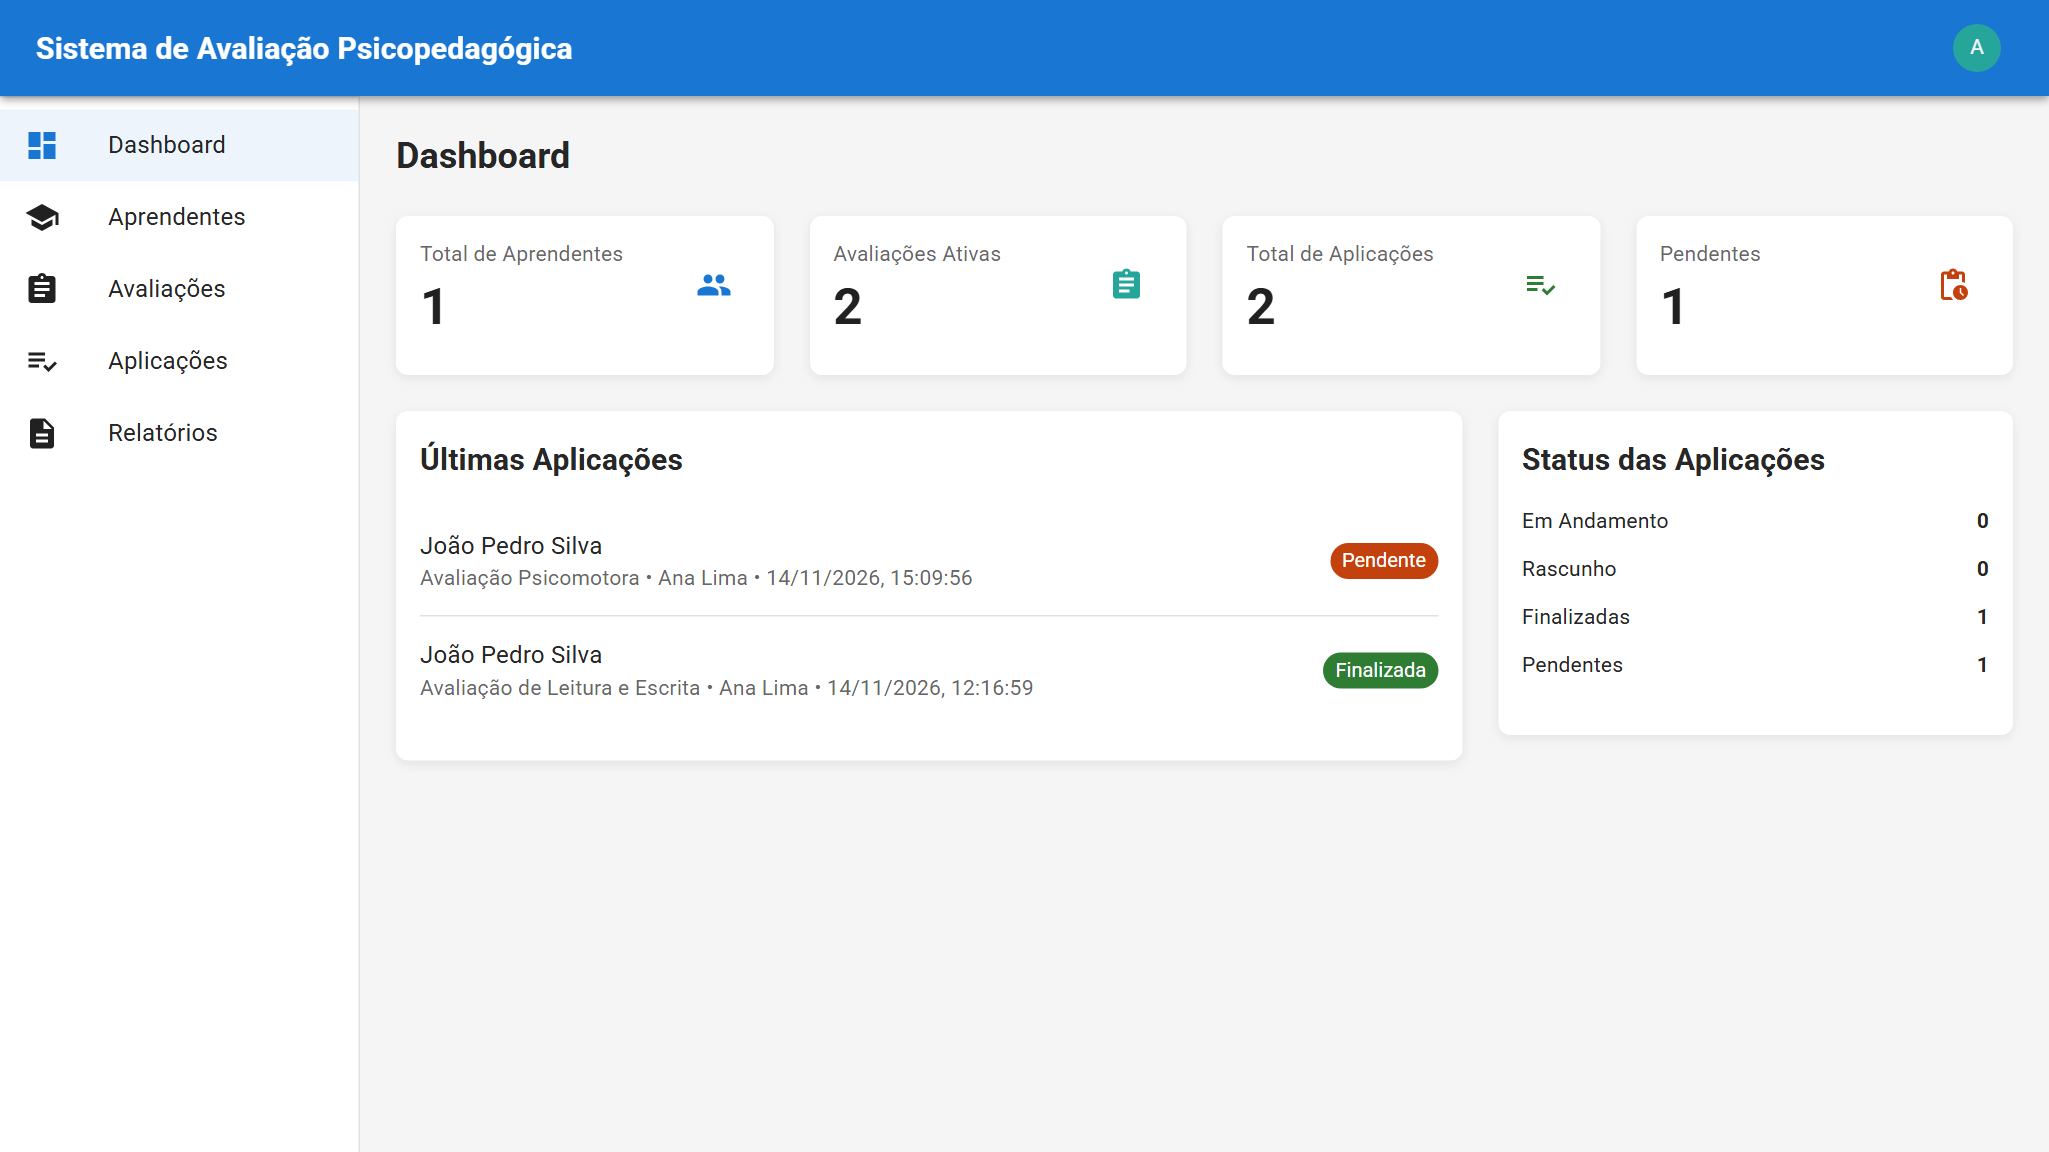
\includegraphics[width=0.90\textwidth]{tela_dashboard.png}
    \caption{Painel inicial do sistema}
    \label{fig:tela_dashboard}
\end{figure}

\begin{figure}[H]
    \centering
    \includegraphics[width=0.90\textwidth]{tela_aprendente.png}
    \caption{Página de detalhe do aprendente}
    \label{fig:tela_aprendente}
\end{figure}

\begin{figure}[H]
    \centering
    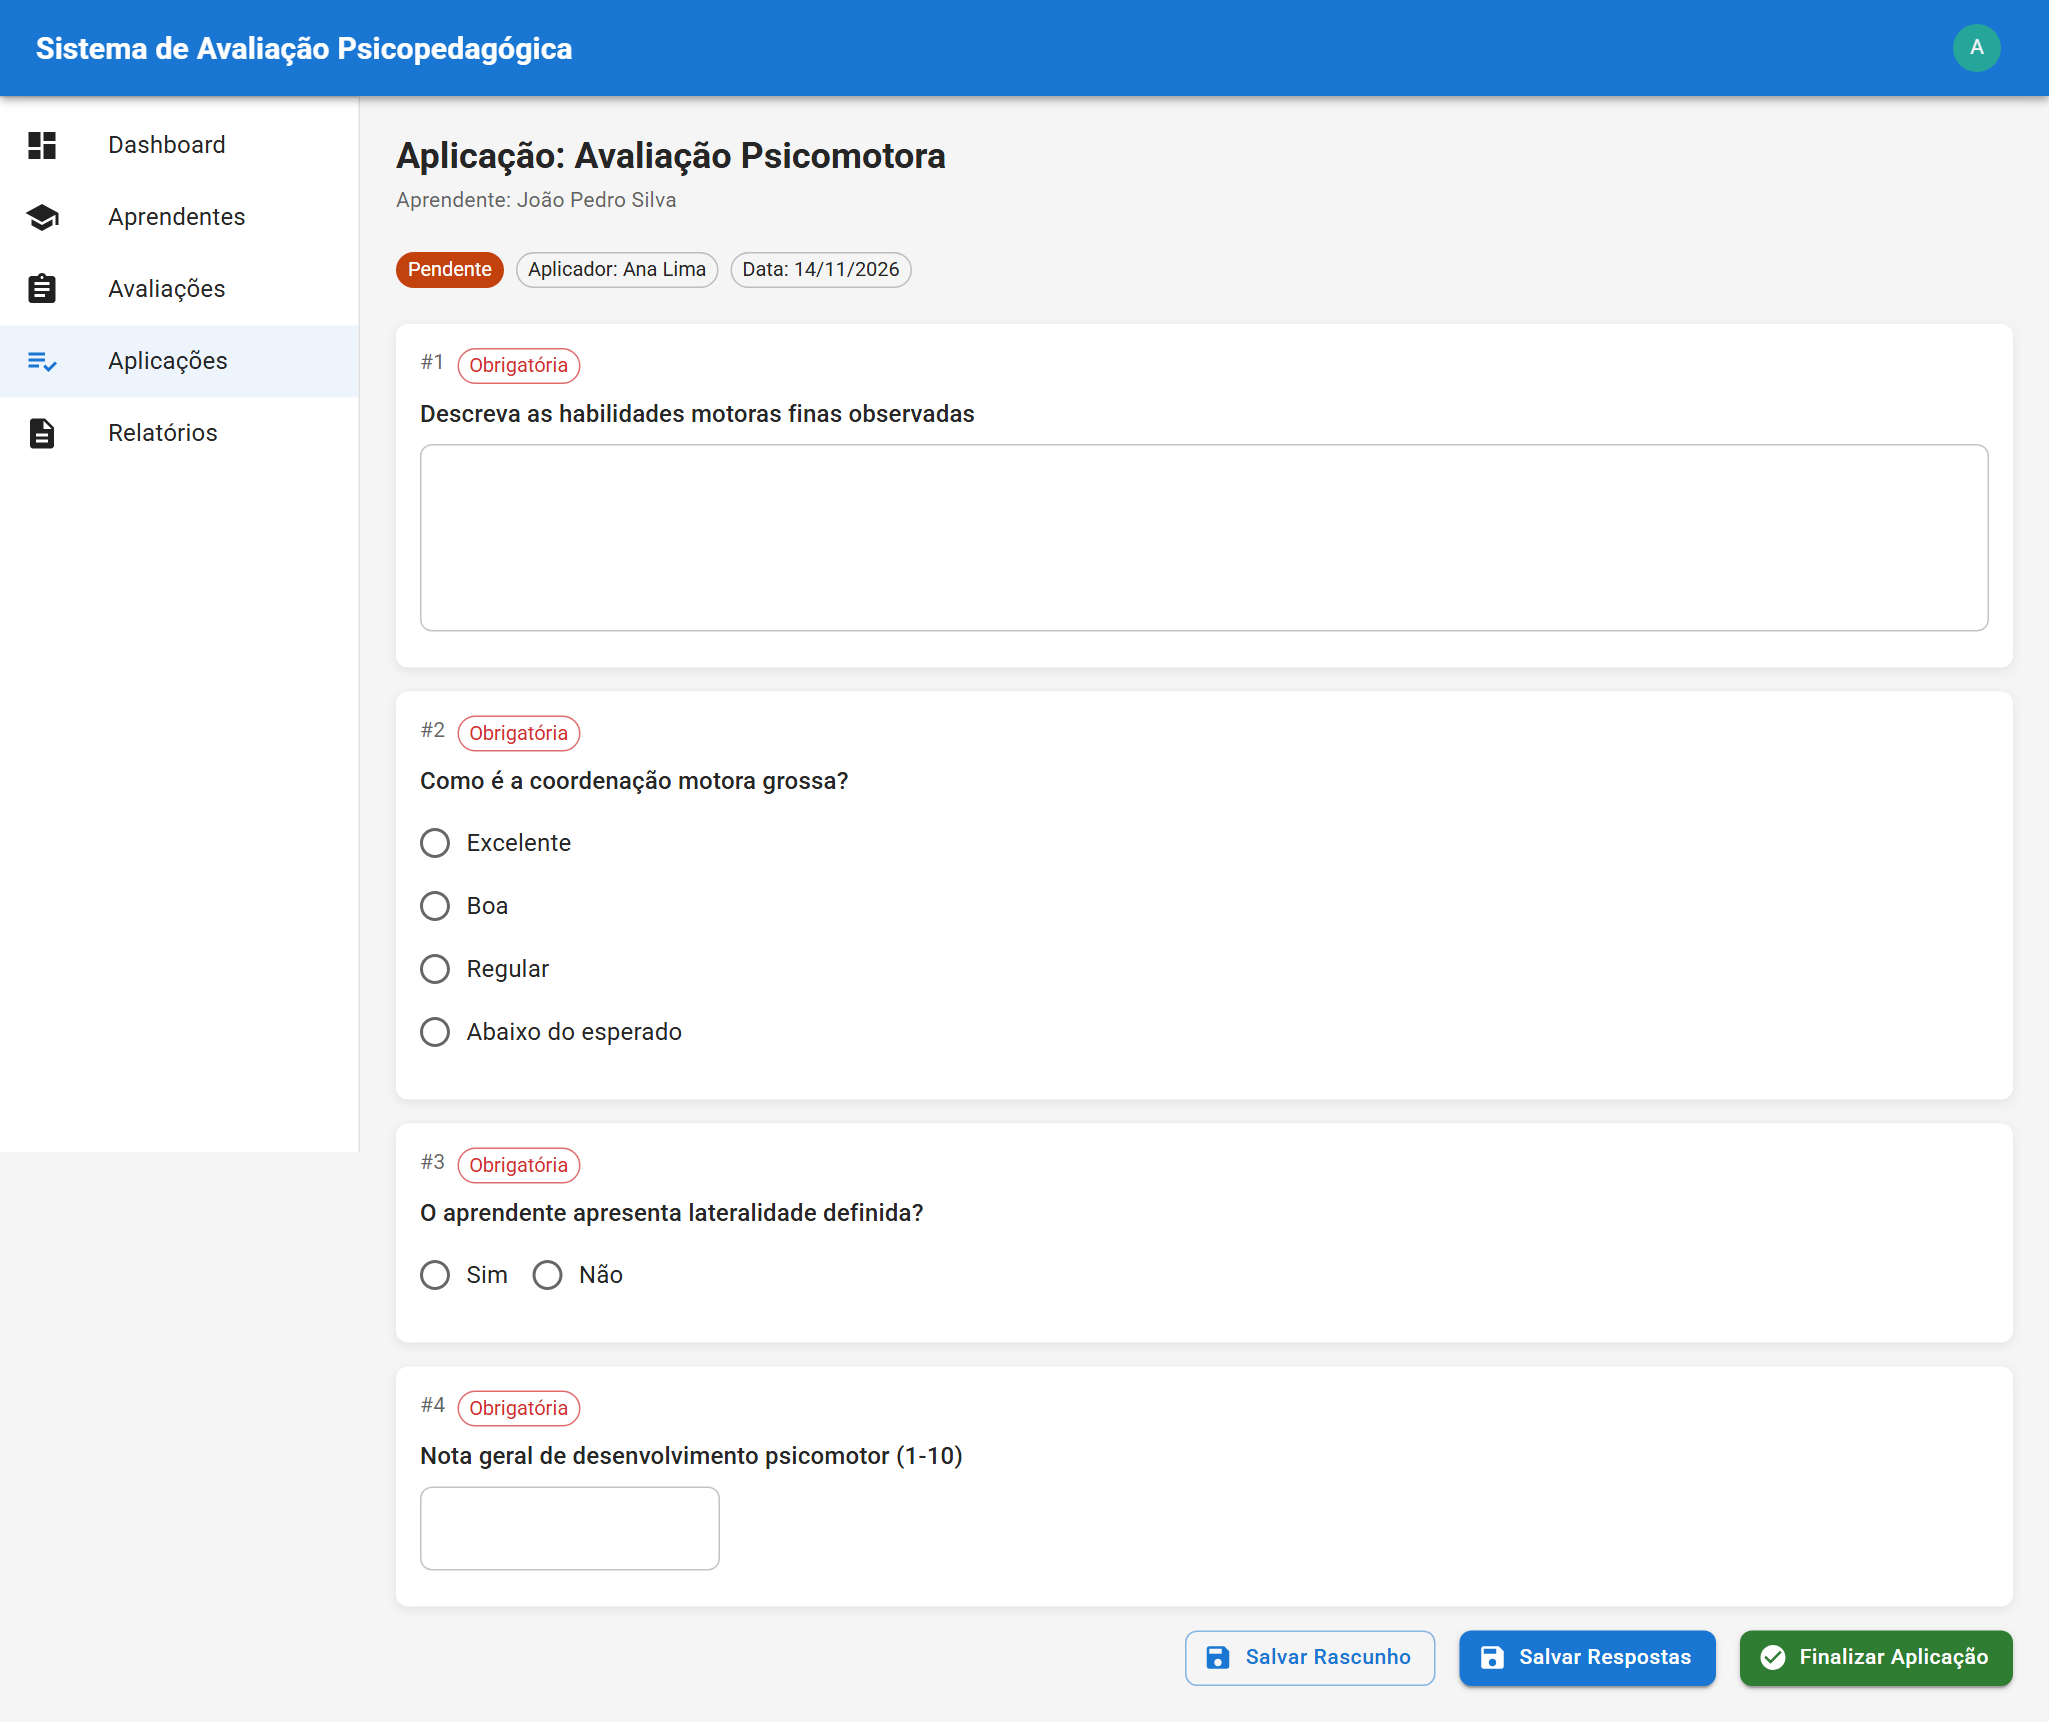
\includegraphics[width=0.90\textwidth]{tela_aplicacao.png}
    \caption{Preenchimento de respostas durante a aplicação de um instrumento}
    \label{fig:tela_aplicacao}
\end{figure}

\begin{figure}[H]
    \centering
    \includegraphics[width=0.90\textwidth]{tela_relatorio.png}
    \caption{Elaboração do relatório de avaliação psicopedagógica}
    \label{fig:tela_relatorio}
\end{figure}

Esse fluxo permite concentrar em uma única plataforma as informações relacionadas às etapas de registro e documentação da avaliação, mantendo a associação entre aprendente, instrumento, aplicação, respostas e relatório.

\section{Testes e execução do sistema}\label{sec:testes}

A verificação técnica do sistema foi realizada por meio de testes automatizados no backend e no frontend, utilizando Vitest. No backend, também foi utilizada a biblioteca Supertest para realizar testes das rotas da API. No frontend, foram empregados React Testing Library e jsdom para verificar o comportamento dos componentes e das funcionalidades da interface.

Conforme o levantamento dos testes realizado durante a análise do código, foram identificados 18 arquivos de teste, sendo nove relacionados ao backend e nove ao frontend. Ao todo, foram executados 127 testes automatizados, dos quais 76 pertenciam ao backend e 51 ao frontend. Todos foram concluídos com sucesso, sem falhas.

A cobertura de código identificada foi de 80,20\% para o backend e 48,37\% para o frontend, considerando a cobertura de linhas e instruções. Esses resultados demonstram que parte significativa das funcionalidades do backend possui testes automatizados, enquanto o frontend ainda apresenta áreas que podem receber maior cobertura.

Além dos testes automatizados, foi realizada a execução prática da plataforma em ambiente Docker, com os serviços necessários para seu funcionamento. Durante essa execução, foi possível utilizar o sistema e verificar seu funcionamento geral, sem ocorrência de problemas que impedissem sua utilização.

\label{sec:avaliacao_usuarios}Para complementar a avaliação técnica, foi aplicado um questionário com profissionais da área de psicopedagogia, com o objetivo de conhecer suas percepções sobre a facilidade de utilização, a organização das informações e a contribuição da plataforma para as atividades de avaliação psicopedagógica.

O questionário foi respondido por cinco participantes, entre os dias 9 e 13 de novembro de 2026. Foram utilizadas sete questões fechadas, avaliadas em uma escala de 1 a 5, em que 1 representava discordância total e 5, concordância total. Também foi disponibilizada uma questão aberta para sugestões de melhorias.

Os resultados das questões fechadas estão apresentados no Quadro \ref{qua:medias_avaliacoes_participantes}.

\begin{quadro}[H]
\centering
\small
\caption{Médias das avaliações dos participantes}
\begin{tabular}{p{13cm} p{2cm}}
\hline
\textbf{Aspecto avaliado} & \textbf{Média} \\
\hline
Facilidade de compreensão e utilização da interface & 4,6 \\
Organização das informações e navegação & 4,6 \\
Cadastro e consulta dos dados dos aprendentes & 4,8 \\
Gerenciamento dos instrumentos avaliativos & 4,2 \\
Registro das aplicações e respostas & 4,4 \\
Geração dos relatórios & 3,8 \\
Contribuição geral da plataforma & 4,6 \\
Média geral & 4,43 \\
\hline
\end{tabular}
\fonte{Elaborado pela autora (2026).}
\label{qua:medias_avaliacoes_participantes}
\end{quadro}

A média geral das respostas foi de 4,43 pontos, indicando uma percepção predominantemente positiva das participantes em relação à plataforma. Das 35 avaliações registradas nas questões fechadas, 33 receberam notas 4 ou 5, correspondendo a 94,3\% das respostas. As duas avaliações restantes receberam nota 3, não havendo respostas com notas 1 ou 2.

O aspecto mais bem avaliado foi o cadastro e a consulta dos dados dos aprendentes, com média de 4,8. A facilidade de utilização, a organização das informações e a contribuição geral da plataforma também apresentaram médias de 4,6.

Por outro lado, a geração dos relatórios obteve a menor média, de 3,8. Embora o resultado ainda seja superior ao ponto intermediário da escala, ele indica uma oportunidade de aprimoramento dessa funcionalidade.

\section{Discussão dos resultados}

Os resultados obtidos demonstram que os principais módulos previstos para a plataforma foram implementados, contemplando o cadastro de aprendentes, o gerenciamento de instrumentos, o registro de aplicações, o armazenamento de respostas e a elaboração de relatórios.

A avaliação realizada com as profissionais complementou os testes técnicos, permitindo observar a percepção das participantes sobre a utilização da plataforma. As médias obtidas foram positivas nos diferentes aspectos avaliados, especialmente no cadastro e na consulta dos aprendentes, na organização das informações e na facilidade de utilização.

A menor média atribuída à geração dos relatórios está relacionada às sugestões apresentadas na questão aberta. Entre as contribuições, foram mencionadas a possibilidade de organizar o relatório em seções predefinidas, incluindo campos para hipótese diagnóstica e encaminhamentos, e a inclusão de recursos que facilitem o preenchimento das informações profissionais.

Também foram sugeridas funcionalidades para ampliar a documentação dos aprendentes, como a possibilidade de anexar laudos, pareceres escolares e registros de avaliações que utilizam protocolos específicos. Outras sugestões envolveram a inclusão de campos para planejamento das intervenções e registro dos objetivos de cada sessão, além de uma linha do tempo para acompanhamento do histórico e do progresso do aprendente.

Essas contribuições apontam que, além do registro das aplicações e dos relatórios, existe interesse em recursos que apoiem a organização de informações complementares e o acompanhamento longitudinal do processo avaliativo.

A implementação do versionamento dos instrumentos representa outro recurso importante para a rastreabilidade das avaliações, pois permite preservar a versão utilizada em aplicações anteriores. Entretanto, o mecanismo ainda apresenta limitações: alterações realizadas antes de existir uma aplicação vinculada podem sobrescrever as questões existentes, e não há recursos completos para registrar justificativas de alterações ou comparar versões.

Outro aspecto relevante é o controle de acesso aos dados dos aprendentes. A restrição de acesso por profissional contribui para a separação dos registros e para a proteção das informações armazenadas. O sistema também conta com autenticação baseada em JWT, validação de dados e registros de auditoria para determinadas operações de acesso e alteração.

A funcionalidade de auditoria permite acompanhar eventos relacionados à utilização do sistema e às modificações realizadas nos registros. Sua implementação foi incorporada ao código versionado do projeto. Apesar disso, a abrangência e a integridade dos registros ainda podem ser aprimoradas, de modo a ampliar a rastreabilidade das operações.

Em relação à consulta histórica, a plataforma disponibiliza registros textuais associados ao histórico do aprendente. Contudo, as aplicações e os relatórios ainda não são apresentados de forma integrada na página individual do aprendente, e as listagens correspondentes não possuem filtros específicos por aprendente. Essa limitação também se relaciona à sugestão das participantes de disponibilizar uma linha do tempo ou histórico visual.

Os relatórios permitem documentar observações e conclusões elaboradas pelo profissional, mantendo a interpretação dos resultados sob sua responsabilidade. Essa característica está alinhada à proposta do sistema, que busca apoiar a organização das informações sem realizar diagnósticos ou interpretações automáticas.

É necessário considerar que a avaliação contou com cinco participantes, constituindo uma amostra reduzida. Portanto, os resultados representam as percepções das profissionais que responderam ao questionário e não permitem generalizações para todo o público de psicopedagogos. Ainda assim, as respostas forneceram indicações relevantes sobre a experiência de utilização e possíveis melhorias.

Em relação aos estudos apresentados no Capítulo~\ref{capitulo2}, o sistema desenvolvido compartilha com \citeonline{abreu2025_sistemas_web_gestao} e \citeonline{pedroso2025_integraedu} a ênfase na centralização de dados e no controle de acesso por perfil como requisitos essenciais de sistemas web voltados à educação. Assim como o IntegraEDU \cite{pedroso2025_integraedu}, o sistema adota perfis diferenciados e restringe a visibilidade dos registros ao usuário responsável. Em relação a \citeonline{carneiro2023_taep4}, que documenta a TAEP4.0, ambos convergem na necessidade de registro estruturado e exportação de relatórios; a diferença está no foco: enquanto a TAEP4.0 apoia a prática docente em sala de aula, este sistema é orientado ao processo clínico-pedagógico da avaliação psicopedagógica. Quanto ao aplicativo de \citeonline{silva2024_app_tdah}, a semelhança está na adoção de formulários personalizáveis e na validação com usuários especialistas; o presente trabalho expande esse escopo ao contemplar múltiplos instrumentos, versionamento e registro longitudinal.

A lacuna identificada na síntese do cap. 2 — ausência de ferramentas específicas para avaliação psicopedagógica na Educação Infantil — é o ponto central que distingue este trabalho dos demais: nenhum dos estudos analisados combina instrumentos configuráveis, versionamento automático com rastreabilidade, registro de auditoria de dados de saúde infantil e geração de relatório clínico vinculado à aplicação. Os resultados da avaliação com as profissionais, em especial a média de 4,43/5,0 e as sugestões de evolução, indicam que o sistema representa uma contribuição concreta nessa direção, ainda que em estágio de protótipo.

De modo geral, os resultados técnicos e a avaliação das participantes indicam que a plataforma apresenta funcionalidades capazes de apoiar a organização e a documentação das atividades de avaliação psicopedagógica. As sugestões recebidas também permitiram identificar aspectos que podem ser desenvolvidos em versões futuras.

\section{Limitações e trabalhos futuros}\label{sec:limitacoes}

Embora as funcionalidades principais tenham sido implementadas e a avaliação inicial tenha apresentado resultados positivos, foram identificadas limitações que podem orientar a continuidade do projeto.

Entre as possibilidades de evolução, destacam-se:

\begin{itemize}
    \item Aprimoramento do histórico do aprendente: integrar as aplicações e os relatórios à página individual do aprendente, além de implementar filtros e uma linha do tempo que facilitem a consulta dos registros.
    \item Evolução do versionamento dos instrumentos: incluir um campo para que o profissional registre a justificativa textual de cada adaptação, permitir a comparação direta entre versões e ampliar o controle sobre as alterações realizadas.
    \item Aprimoramento da auditoria: ampliar a cobertura dos eventos registrados e fortalecer os mecanismos de integridade e consulta dos logs.
    \item Aprimoramento da segurança: implementar medidas adicionais de proteção dos dados, incluindo configurações de comunicação segura e políticas de retenção e exclusão.
    \item Evolução dos relatórios: implementar seções predefinidas, como hipótese diagnóstica e encaminhamentos, além de ampliar as possibilidades de formatação e organização dos documentos.
    \item Anexos e documentação complementar: permitir o armazenamento de arquivos relacionados ao aprendente, como laudos, pareceres escolares e registros de avaliações realizadas com protocolos específicos.
    \item Planejamento das intervenções: disponibilizar campos para registrar os objetivos de cada sessão e o planejamento das intervenções propostas pelo profissional.
\end{itemize}

Dessa forma, o sistema desenvolvido atende ao propósito de oferecer uma ferramenta para apoiar a organização e a documentação das etapas da avaliação psicopedagógica. Os testes técnicos e a avaliação inicial com profissionais forneceram evidências favoráveis ao funcionamento e à utilidade percebida da plataforma. As limitações identificadas e as sugestões recebidas constituem possibilidades de aprimoramento para versões futuras.
\chapter[Conclusão]{Conclusão} \label{capitulo7}

O presente trabalho teve como objetivo desenvolver um sistema web de apoio à avaliação psicopedagógica na educação infantil, buscando oferecer uma ferramenta para auxiliar os profissionais na organização das informações dos aprendentes, no gerenciamento de instrumentos avaliativos, no registro das aplicações e na elaboração de relatórios. Esta conclusão retoma cada objetivo específico, sintetiza as limitações identificadas e aponta os trabalhos futuros.

\section{Atendimento aos objetivos específicos}

O primeiro objetivo — identificar instrumentos e métodos empregados na avaliação psicopedagógica infantil — foi atendido por meio da revisão bibliográfica apresentada nos Capítulos~\ref{capitulo2} e~\ref{capitulo3-0}, que levantou dimensões cognitivas, emocionais e pedagógicas relevantes e orientou a definição dos requisitos do sistema.

O segundo objetivo — projetar a arquitetura do sistema — foi atendido. A aplicação adota arquitetura em três camadas (apresentação, aplicação e persistência), com backend organizado em sete módulos independentes por domínio funcional (autenticação, aprendentes, avaliações, aplicações, relatórios, auditoria e dashboard), frontend separado em camadas de API, contexto, componentes e páginas, e banco de dados relacional MySQL, conforme descrito nas Seções~\ref{sec:arquitetura} a~\ref{sec:frontend}.

O terceiro objetivo — implementar mecanismos de proteção das informações e analisar a adequação do sistema à LGPD — foi atendido. Foram implementados controle de acesso por perfil e titularidade, hash bcrypt com fator de custo 12 para senhas, exclusão lógica e registro de auditoria das operações e consultas a dados clínicos. A análise apresentada na Seção~\ref{sec:seguranca} identificou as medidas ainda necessárias para o uso com dados reais: o sistema não implementa criptografia em repouso dos campos sensíveis, não registra o consentimento do responsável legal nem a base legal do tratamento, não define política de retenção, descarte e backup dos dados e não possui mecanismo de exclusão definitiva. Por isso, o sistema não deve ser considerado em conformidade com a LGPD no estágio atual; trata-se de um protótipo que não está preparado para uso em produção com dados reais sem o endereçamento dessas limitações.

O quarto objetivo — desenvolver uma interface orientada à usabilidade e à acessibilidade — foi atendido, com a ressalva descrita adiante quanto à acessibilidade. Quanto à usabilidade, a média geral de 4,43/5,0 no questionário com cinco profissionais, com 94,3\% das respostas nas notas 4 ou 5, indica adequação percebida ao contexto clínico-pedagógico; o aspecto com menor média foi a geração de relatórios (3,8), que concentrou as sugestões de melhoria. Quanto à acessibilidade, a avaliação automatizada com o axe-core em 18 telas identificou inicialmente cinco tipos de violação dos critérios A e AA das WCAG 2.2, dois deles de impacto crítico: o botão de exibir senha sem nome acessível e os campos de resposta da aplicação sem rótulo associado ao enunciado da questão. Após as correções, uma nova execução não identificou violações (Seção~\ref{sec:acessibilidade}). A ressalva é que a verificação foi apenas automatizada: não foram realizados testes manuais de navegação por teclado nem com leitores de tela, de modo que não é possível afirmar conformidade plena com as diretrizes.

O quinto objetivo — realizar testes com especialistas — foi atendido. Foram aplicados 127 testes automatizados (76 no backend, 51 no frontend), todos com sucesso, com cobertura de 80,20\% de linhas no backend. O questionário foi respondido por cinco profissionais entre 9 e 13 de novembro de 2026. A amostra reduzida é uma limitação reconhecida: os resultados não permitem generalizações para todo o público de psicopedagogos.

O sexto objetivo — analisar o impacto potencial sobre as práticas avaliativas — foi atendido na discussão do Capítulo~\ref{capitulo6}, onde os resultados são comparados com os estudos relacionados e discutidas as contribuições e limitações do sistema frente ao estado da arte.

\section{Limitações}

Além das limitações já mencionadas em relação ao objetivo três, o sistema apresenta as seguintes restrições que precisam ser consideradas:

\begin{itemize}
    \item \textbf{Auditoria de acessos}: o registro de auditoria implementado tem limitações de integridade — é gravado em conexão separada à operação, sem encadeamento criptográfico, e pode ser modificado por acesso direto ao banco. Não há política de retenção para os próprios registros de auditoria.
    \item \textbf{Criptografia em repouso}: os dados armazenados no banco não são criptografados em nível de campo. Campos sensíveis — textos de histórico, respostas e relatórios — ficam em texto plano, protegidos apenas pelos controles de acesso à infraestrutura.
    \item \textbf{Ausência de interoperabilidade}: o sistema não exporta nem importa dados em formatos padronizados (como HL7 FHIR ou CSV estruturado), dificultando a integração com outros sistemas de saúde ou educação.
    \item \textbf{Ambiente local}: o sistema foi validado apenas em ambiente Docker local. Não foi realizado deploy em ambiente de produção nem avaliação de desempenho sob carga real.
    \item \textbf{Acessibilidade}: a avaliação foi apenas automatizada; não foram realizados testes manuais de navegação por teclado, com leitores de tela nem com pessoas com deficiência.
    \item \textbf{Validação com amostra reduzida}: a avaliação contou com cinco participantes, sem aleatorização ou grupo de controle, o que limita a validade externa dos resultados de usabilidade.
    \item \textbf{RF09 parcialmente atendido}: o versionamento automático preserva as questões usadas em cada aplicação, mas o sistema não disponibiliza campo para que o profissional registre textualmente a justificativa da adaptação.
    \item \textbf{RF12 parcialmente atendido}: aplicações e relatórios não estão integrados à página individual do aprendente; a consulta longitudinal exige navegação entre módulos separados.
\end{itemize}

\section{Trabalhos futuros}

Com base nas limitações identificadas e nas sugestões das profissionais participantes, os principais trabalhos futuros incluem:

\begin{itemize}
    \item Implementar criptografia em repouso dos campos sensíveis e definir política de retenção e descarte dos dados, habilitando o sistema para uso em produção com dados reais de crianças.
    \item Complementar a avaliação automatizada de acessibilidade com testes manuais de navegação por teclado e leitores de tela e, se possível, com pessoas com deficiência, e incorporar a verificação com o axe-core aos testes automatizados do frontend, evitando regressões.
    \item Integrar aplicações e relatórios à página individual do aprendente, com linha do tempo que facilite a consulta longitudinal do histórico avaliativo.
    \item Permitir a definição de regras de pontuação no cadastro dos instrumentos, para que o sistema calcule automaticamente os escores das aplicações, tarefa apontada como custosa pelos profissionais em trabalhos relacionados \cite{valgas2021_prontuario_neuropsicologico}.
    \item Adicionar campo de justificativa textual ao versionamento de instrumentos, permitindo que o profissional registre a motivação de cada adaptação.
    \item Expandir o módulo de relatórios com seções predefinidas (hipótese diagnóstica, encaminhamentos, objetivos de intervenção) e suporte a anexos (laudos, pareceres escolares).
    \item Implementar a exportação dos dados em formato estruturado e estudar a interoperabilidade com sistemas de saúde e plataformas educacionais, avaliando a adoção de padrões de dados em saúde, como o HL7 FHIR \cite{Lins_Ferreira_Nutels_Junior_Tenorio_Filho_2024}, necessidade também apontada por trabalhos relacionados \cite{valgas2021_prontuario_neuropsicologico}.
    \item Realizar nova avaliação de usabilidade com amostra maior e mais diversificada de profissionais, em ambiente de produção.
    \item Realizar deploy em ambiente de nuvem e avaliar desempenho e disponibilidade sob carga real.
\end{itemize}

\section{Considerações finais}

Conclui-se que o objetivo geral do trabalho foi alcançado: foi desenvolvido um sistema web funcional que reúne recursos para apoiar a organização e a documentação das etapas da avaliação psicopedagógica na educação infantil. Os testes automatizados e a avaliação com profissionais forneceram evidências favoráveis ao funcionamento e à utilidade percebida da plataforma. As limitações identificadas — especialmente as relacionadas à proteção de dados, à interoperabilidade e ao escopo da validação — delimitam claramente o caráter de protótipo do sistema e orientam a agenda de desenvolvimento para versões futuras.

% ----------------------------------------------------------
% ELEMENTOS PÓS-TEXTUAIS
% ----------------------------------------------------------
\postextual
% ----------------------------------------------------------

% ----------------------------------------------------------
% Referências bibliográficas
% ----------------------------------------------------------
\bibliography{bibliografia}

% ----------------------------------------------------------
% Glossário
% ----------------------------------------------------------
% Consulte o manual da classe abntex2 para orientações sobre o glossário.
%\glossary

% Apêndices: o ambiente apendicesenv gera "APÊNDICE A – Título",
% atualiza o cabeçalho das páginas e faz o \ref devolver A, B...
% Nos arquivos dos apêndices use \chapter{...} (sem asterisco) + \label.
\begin{apendicesenv}
\chapter*{Apêndice A - Termo de Consentimento Livre e Esclarecido}
\addcontentsline{toc}{chapter}{Apêndice A - Termo de Consentimento Livre e Esclarecido}
\label{apendice:tcle}

\textbf{Título da pesquisa:} Desenvolvimento de um sistema web de apoio à avaliação psicopedagógica na Educação Infantil

\textbf{Pesquisadora responsável:} Sanielle Azara

\textbf{Instituição:} Universidade do Estado de Minas Gerais (UEMG)

\bigskip

Você está sendo convidada a participar, como voluntária, de uma pesquisa de natureza aplicada que tem como objetivo desenvolver um sistema web para apoiar a organização e o registro das atividades de avaliação psicopedagógica. Sua participação consiste em conceder uma entrevista semiestruturada sobre sua prática profissional, com foco nas ferramentas atualmente utilizadas para registro dos atendimentos, uso de instrumentos avaliativos e elaboração de relatórios.

\bigskip
\textbf{Sobre sua participação:}

\begin{itemize}
    \item A participação é voluntária. Você poderá recusar-se a responder qualquer pergunta ou interromper a entrevista a qualquer momento, sem qualquer prejuízo.
    \item A entrevista terá duração estimada de 20 a 30 minutos.
    \item As informações fornecidas serão utilizadas exclusivamente para fins desta pesquisa, na etapa de levantamento de requisitos do sistema.
    \item Seus dados de identificação não serão divulgados no trabalho. As informações coletadas poderão ser mencionadas de forma genérica, sem referência a nome, instituição ou qualquer dado que permita sua identificação.
    \item Não há riscos previsíveis associados à sua participação. Não há benefício direto para a participante, mas os resultados poderão contribuir para o desenvolvimento de ferramentas mais adequadas à prática psicopedagógica.
\end{itemize}

\bigskip
\textbf{Contato:}

Em caso de dúvidas sobre a pesquisa, entre em contato com a pesquisadora responsável pelo endereço eletrônico: \texttt{sanielle.azara@gmail.com}.

\bigskip

Declaro que fui informada sobre os objetivos e procedimentos desta pesquisa, que compreendi as informações acima e que concordo em participar voluntariamente.

\bigskip
\bigskip

\noindent
\begin{minipage}{0.45\textwidth}
    \centering
    \rule{6cm}{0.4pt}\\
    Assinatura da participante\\
    \bigskip
    Data: \underline{\hspace{3cm}}
\end{minipage}
\hfill
\begin{minipage}{0.45\textwidth}
    \centering
    \rule{6cm}{0.4pt}\\
    Assinatura da pesquisadora\\
    \bigskip
    Data: \underline{\hspace{3cm}}
\end{minipage}

\chapter*{Apêndice B - Questionário de Avaliação do Sistema}
\addcontentsline{toc}{chapter}{Apêndice B - Questionário de Avaliação do Sistema}
\label{apendice:questionario}

Este questionário foi aplicado de forma anônima a profissionais da área de psicopedagogia após a utilização do sistema web desenvolvido. Teve como objetivo coletar percepções sobre a facilidade de uso, a organização das informações e a adequação da plataforma às atividades de avaliação psicopedagógica.

\bigskip
\textbf{Instruções:} Para cada afirmação abaixo, indique seu grau de concordância em uma escala de 1 a 5, em que:

\begin{center}
\textbf{1} = Discordo totalmente \quad \textbf{2} = Discordo \quad \textbf{3} = Neutro \quad \textbf{4} = Concordo \quad \textbf{5} = Concordo totalmente
\end{center}

\bigskip

\begin{enumerate}

    \item A interface do sistema é de fácil compreensão e utilização.

    \bigskip
    \noindent
    \begin{tabular}{ccccc}
        \quad(\ \ ) 1 \quad & \quad(\ \ ) 2 \quad & \quad(\ \ ) 3 \quad & \quad(\ \ ) 4 \quad & \quad(\ \ ) 5 \quad
    \end{tabular}

    \bigskip

    \item As informações estão organizadas de forma clara e a navegação entre as telas é intuitiva.

    \bigskip
    \noindent
    \begin{tabular}{ccccc}
        \quad(\ \ ) 1 \quad & \quad(\ \ ) 2 \quad & \quad(\ \ ) 3 \quad & \quad(\ \ ) 4 \quad & \quad(\ \ ) 5 \quad
    \end{tabular}

    \bigskip

    \item O cadastro e a consulta dos dados dos aprendentes atendem às necessidades do processo de avaliação.

    \bigskip
    \noindent
    \begin{tabular}{ccccc}
        \quad(\ \ ) 1 \quad & \quad(\ \ ) 2 \quad & \quad(\ \ ) 3 \quad & \quad(\ \ ) 4 \quad & \quad(\ \ ) 5 \quad
    \end{tabular}

    \bigskip

    \item O gerenciamento dos instrumentos avaliativos (criação, edição e versionamento) é adequado à prática profissional.

    \bigskip
    \noindent
    \begin{tabular}{ccccc}
        \quad(\ \ ) 1 \quad & \quad(\ \ ) 2 \quad & \quad(\ \ ) 3 \quad & \quad(\ \ ) 4 \quad & \quad(\ \ ) 5 \quad
    \end{tabular}

    \bigskip

    \item O registro das aplicações e das respostas é adequado para documentar os atendimentos realizados.

    \bigskip
    \noindent
    \begin{tabular}{ccccc}
        \quad(\ \ ) 1 \quad & \quad(\ \ ) 2 \quad & \quad(\ \ ) 3 \quad & \quad(\ \ ) 4 \quad & \quad(\ \ ) 5 \quad
    \end{tabular}

    \bigskip

    \item A geração dos relatórios atende às necessidades de elaboração de devolutivas profissionais.

    \bigskip
    \noindent
    \begin{tabular}{ccccc}
        \quad(\ \ ) 1 \quad & \quad(\ \ ) 2 \quad & \quad(\ \ ) 3 \quad & \quad(\ \ ) 4 \quad & \quad(\ \ ) 5 \quad
    \end{tabular}

    \bigskip

    \item De forma geral, a plataforma contribui para a organização e o acompanhamento das atividades de avaliação psicopedagógica.

    \bigskip
    \noindent
    \begin{tabular}{ccccc}
        \quad(\ \ ) 1 \quad & \quad(\ \ ) 2 \quad & \quad(\ \ ) 3 \quad & \quad(\ \ ) 4 \quad & \quad(\ \ ) 5 \quad
    \end{tabular}

    \bigskip

    \item Você identificou dificuldades, limitações ou tem sugestões de melhoria para o sistema? Descreva livremente.

    \bigskip
    \noindent\rule{\textwidth}{0.4pt}

    \bigskip
    \noindent\rule{\textwidth}{0.4pt}

    \bigskip
    \noindent\rule{\textwidth}{0.4pt}

    \bigskip
    \noindent\rule{\textwidth}{0.4pt}

\end{enumerate}

\bigskip
\noindent\textit{Este questionário é anônimo. Nenhuma informação que permita identificar o respondente será coletada ou divulgada.}

\end{apendicesenv}

% ---
% Anexos
%\begin{anexosenv}

% Imprime uma página indicando o início dos anexos
\partanexos

\chapter{1}
Texto

\chapter{2}
Texto

\chapter{3}
Texto

\end{anexosenv}


\end{document}